
\chapter{Ferromagnetismo} % Main chapter title

\begin{figure}[H]
    \centering
    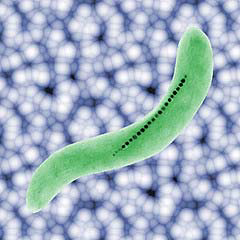
\includegraphics[width=0.8\textwidth]{./Figures/bacteriaMagnetica}
	\caption{bacteria Magnética}
	\label{fig:bacteriaMagnetica}
\end{figure}

\begin{center}

Fue de casa en casa arrastrando dos lingotes metálicos, y todo el mundo se
espantó al ver que los calderos, las pailas, las tenazas y los anafes se caían de su sitio, y las maderas crujían por la desesperación de los clavos y los tornillos tratando de desenclavarse, y aun los objetos perdidos desde hacía mucho tiempo aparecían por donde más se les había buscado, y se arrastraban en desbandada turbulenta detrás de los fierros mágicos de Melquíades. "Las cosas tienen vida propia -pregonaba el gitano con áspero acento-, todo es cuestión de despertarles el ánima".

\hspace{6.6cm} Cien años de soledad\\
\hspace{7.6cm} Garcia Márquez

\end{center}

%\large
%\textbf{Ferromagnetismo}
%\normalsize

\section{Concepto de Ferromagnetismo}

\textbf{El ferromagnetismo es un fenómeno social, no existe el ferromagnetismo en átomos aislados, solo se da, cuando los átomos de la sustancia pueden interactuar entre ellos.}

\begin{itemize}
	\item El ferromagnetismo es el ordenamiento magnético de todos los momentos magnéticos atómicos en una dada dirección y sentido espontáneamente. Hay varios materiales cristalinos que presentan esta propiedad.
	
	\item El ferromagnetismo no es una propiedad inherente del hierro. Hay aleaciones que no contienen hierro y son ferromagnéticas (aleaciones \textbf{Heusler}, por ejemplo $Cu_{2}MnAl$), por el contrario, tenemos aleaciones de hierro que no son ferromagnéticas (inoxidables austeníticos), incluso, bajo ciertas condiciones el hierro no es ferromagnético.

	\item En los elementos de transición encontramos tres que poseen propiedades ferromagnéticas $Fe(d^{6})$, $Co(d^{7})$, $Ni(d^{8})$ y en los de transición interna el Gadolinio $Gd(f^{8})$ y el Disprosio $Dy(f^{10})$.

	\item En los materiales compuestos hay varios casos más.

\end{itemize}


Antes de comenzar con el tema en cuestión aclaremos algunas ideas Entendemos por fase de una sustancia el cuerpo macroscópico homogéneo. En los puntos de solidificación o ebullición pueden coexistir dos fase, o sea, hay presentes dos tipos de materia homogénea. Algunos metales, por ejemplo el hierro, estaño presentan alotropía o polimorfismo, cristalizan en varias estructura cada una de ellas es una fase. Estas fase se ponen de manifiesto con los cambios de temperatura y son llamados cambios de fase en estado solido El caso que nos interesa es el hierro puro en particular. El comportamiento de este elemento es particular tiene dos estados sólidos la ferrita o hierro alfa de fase cúbica de cuerpo centrado bcc) fase de baja temperatura Posteriormente pasa a otra fase sólida de estructura cubica centrada en el las caras fcc a mayor temperatura llama hierro gama. Si aumentamos mas la temperatura tenemos otra transformación, también de estructura bcc, luego de la cual funde. En la figura \ref{fig:d1} se observa el comportamiento indicado La zona de rallado oblicuo indica la zona ferromagnética y la de rallado horizontal, la zona paramagnética. En un tiempo se pensó que el hierro tenia tres fases de estado solido, posterior mente se vio que el cambio que se produce a la temperatura $T_{c}$ no es un cambio de fase de primer orden como los mencionados Se debe a la transformación ferromagnética paramagnética Dicho de otro modo la transformación magnética ocurre dentro de la fase alfa Vemos que una misma fase puede ser ferromagnética o paramagnética.

\begin{figure}[H]
    \centering
    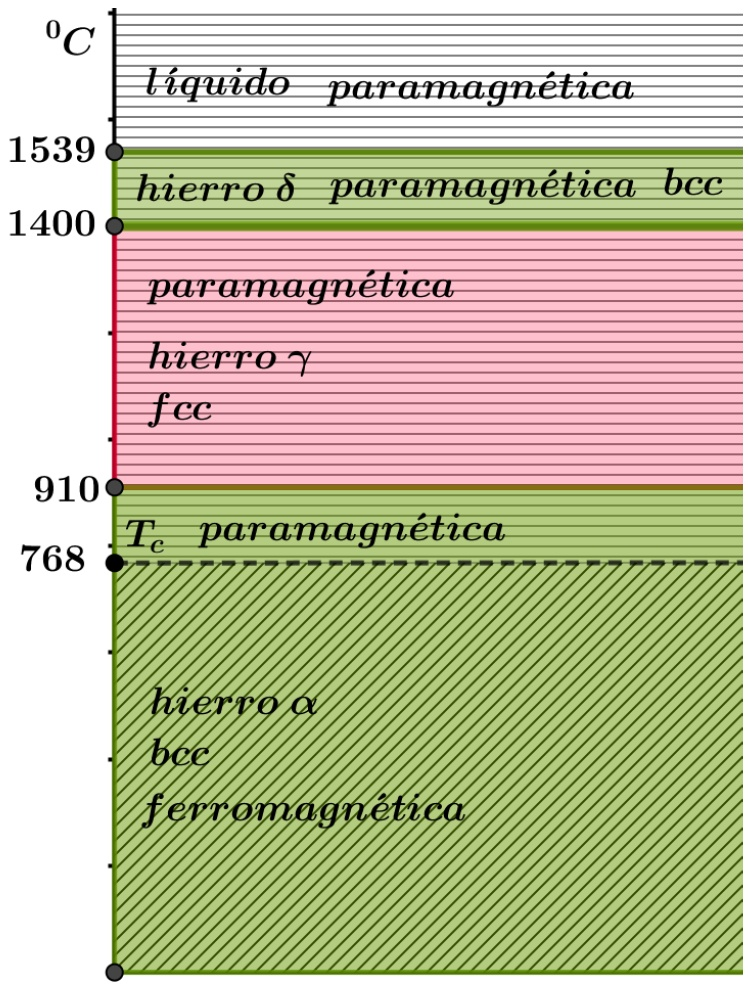
\includegraphics[width=0.6\textwidth]{./Figures/fig_d1}
	\caption{Estados del Hierro}
	\label{fig:d1}
\end{figure}

Tratemos de explicar el comportamiento particular de hierro Recordemos que la propiedad adecuada para definir el equilibrio de un sistema metálico, que nos ofrece la termodinámica es la energía libre $F$, que en el equilibrio tiene un mínimo $F=E-TS$. Se trata de expresar estas variables en función de datos medibles. En un proceso lento, reversible a presión constante Es este el procedimiento formal para encontrar la energía libre. Veámoslo con un poco mas de detalle, sabemos que

\begin{equation}
	dE=dQ+dW=dQ=C_{p}dT \quad\text{si prescindimos del trabajo dW}
\end{equation}

ya que en los metales es pequeño, recordamos que $dS\dfrac{dQ}{T}=C_{p}\dfrac{dT}{T}$. La variación de la $F$ sera:

\begin{equation}
	dF=dE-TdS-SdT=C_{p}T-TC_{p}\dfrac{dT}{T}-SdT=-SdT
\end{equation}


Integrando $F=F_{0}-\int_{0}^{T}SdT$ siendo $F_{0}=E_{0}$ (energía interna de interacción más energía de vibración a $0{^{O}K}$. también tenemos que $S=S_{0}+\int_{0}^{T}C_{p}\dfrac{dT}{T}$, donde $S_{0}$ es la entropía a $0{^{o}K}$, (a esa temperatura no existe desorden y las vibraciones son mínimas) entonces $S_{0}=0$ por lo tanto:

\begin{equation}
	F=E-{0}-\int_{0}^{T}Sdt=E_{0}-\int_{0}^{T}\left[ \int_{0}^{T}C_{p}\dfrac{dT}{T} \right] dT
\end{equation}

Vemos que al aumentar $T$ la energía libre disminuye y más aun, cuando mayor es $C_{p}$, el balance entre $E_{0}$ y $C_{p}$ determinarán en el caso de dos fases, cual tendrá menor energía libre, o sea cual será la estable.





\section{Particularidad del hierro}
Generalmente cuando se baja la temperatura se pasa a una estructura más compacta con un volumen menor. Vemos que no es el caso de la transformación
$\gamma\rightarrow\alpha$. Donde el $Fe\alpha$ tiene el 68\% del volumen total de la celda unitaria ocupada por átomos de hierro. El $Fe\gamma$ el
74\% del volumen total está ocupado por átomos de hierro. Podemos concluir, pues, que el $Fe\gamma$ es más denso que el $Fe\alpha$ (para una misma cantidad de volumen, habrá más masa de $Fe$).

\begin{figure}[H]
    \centering
    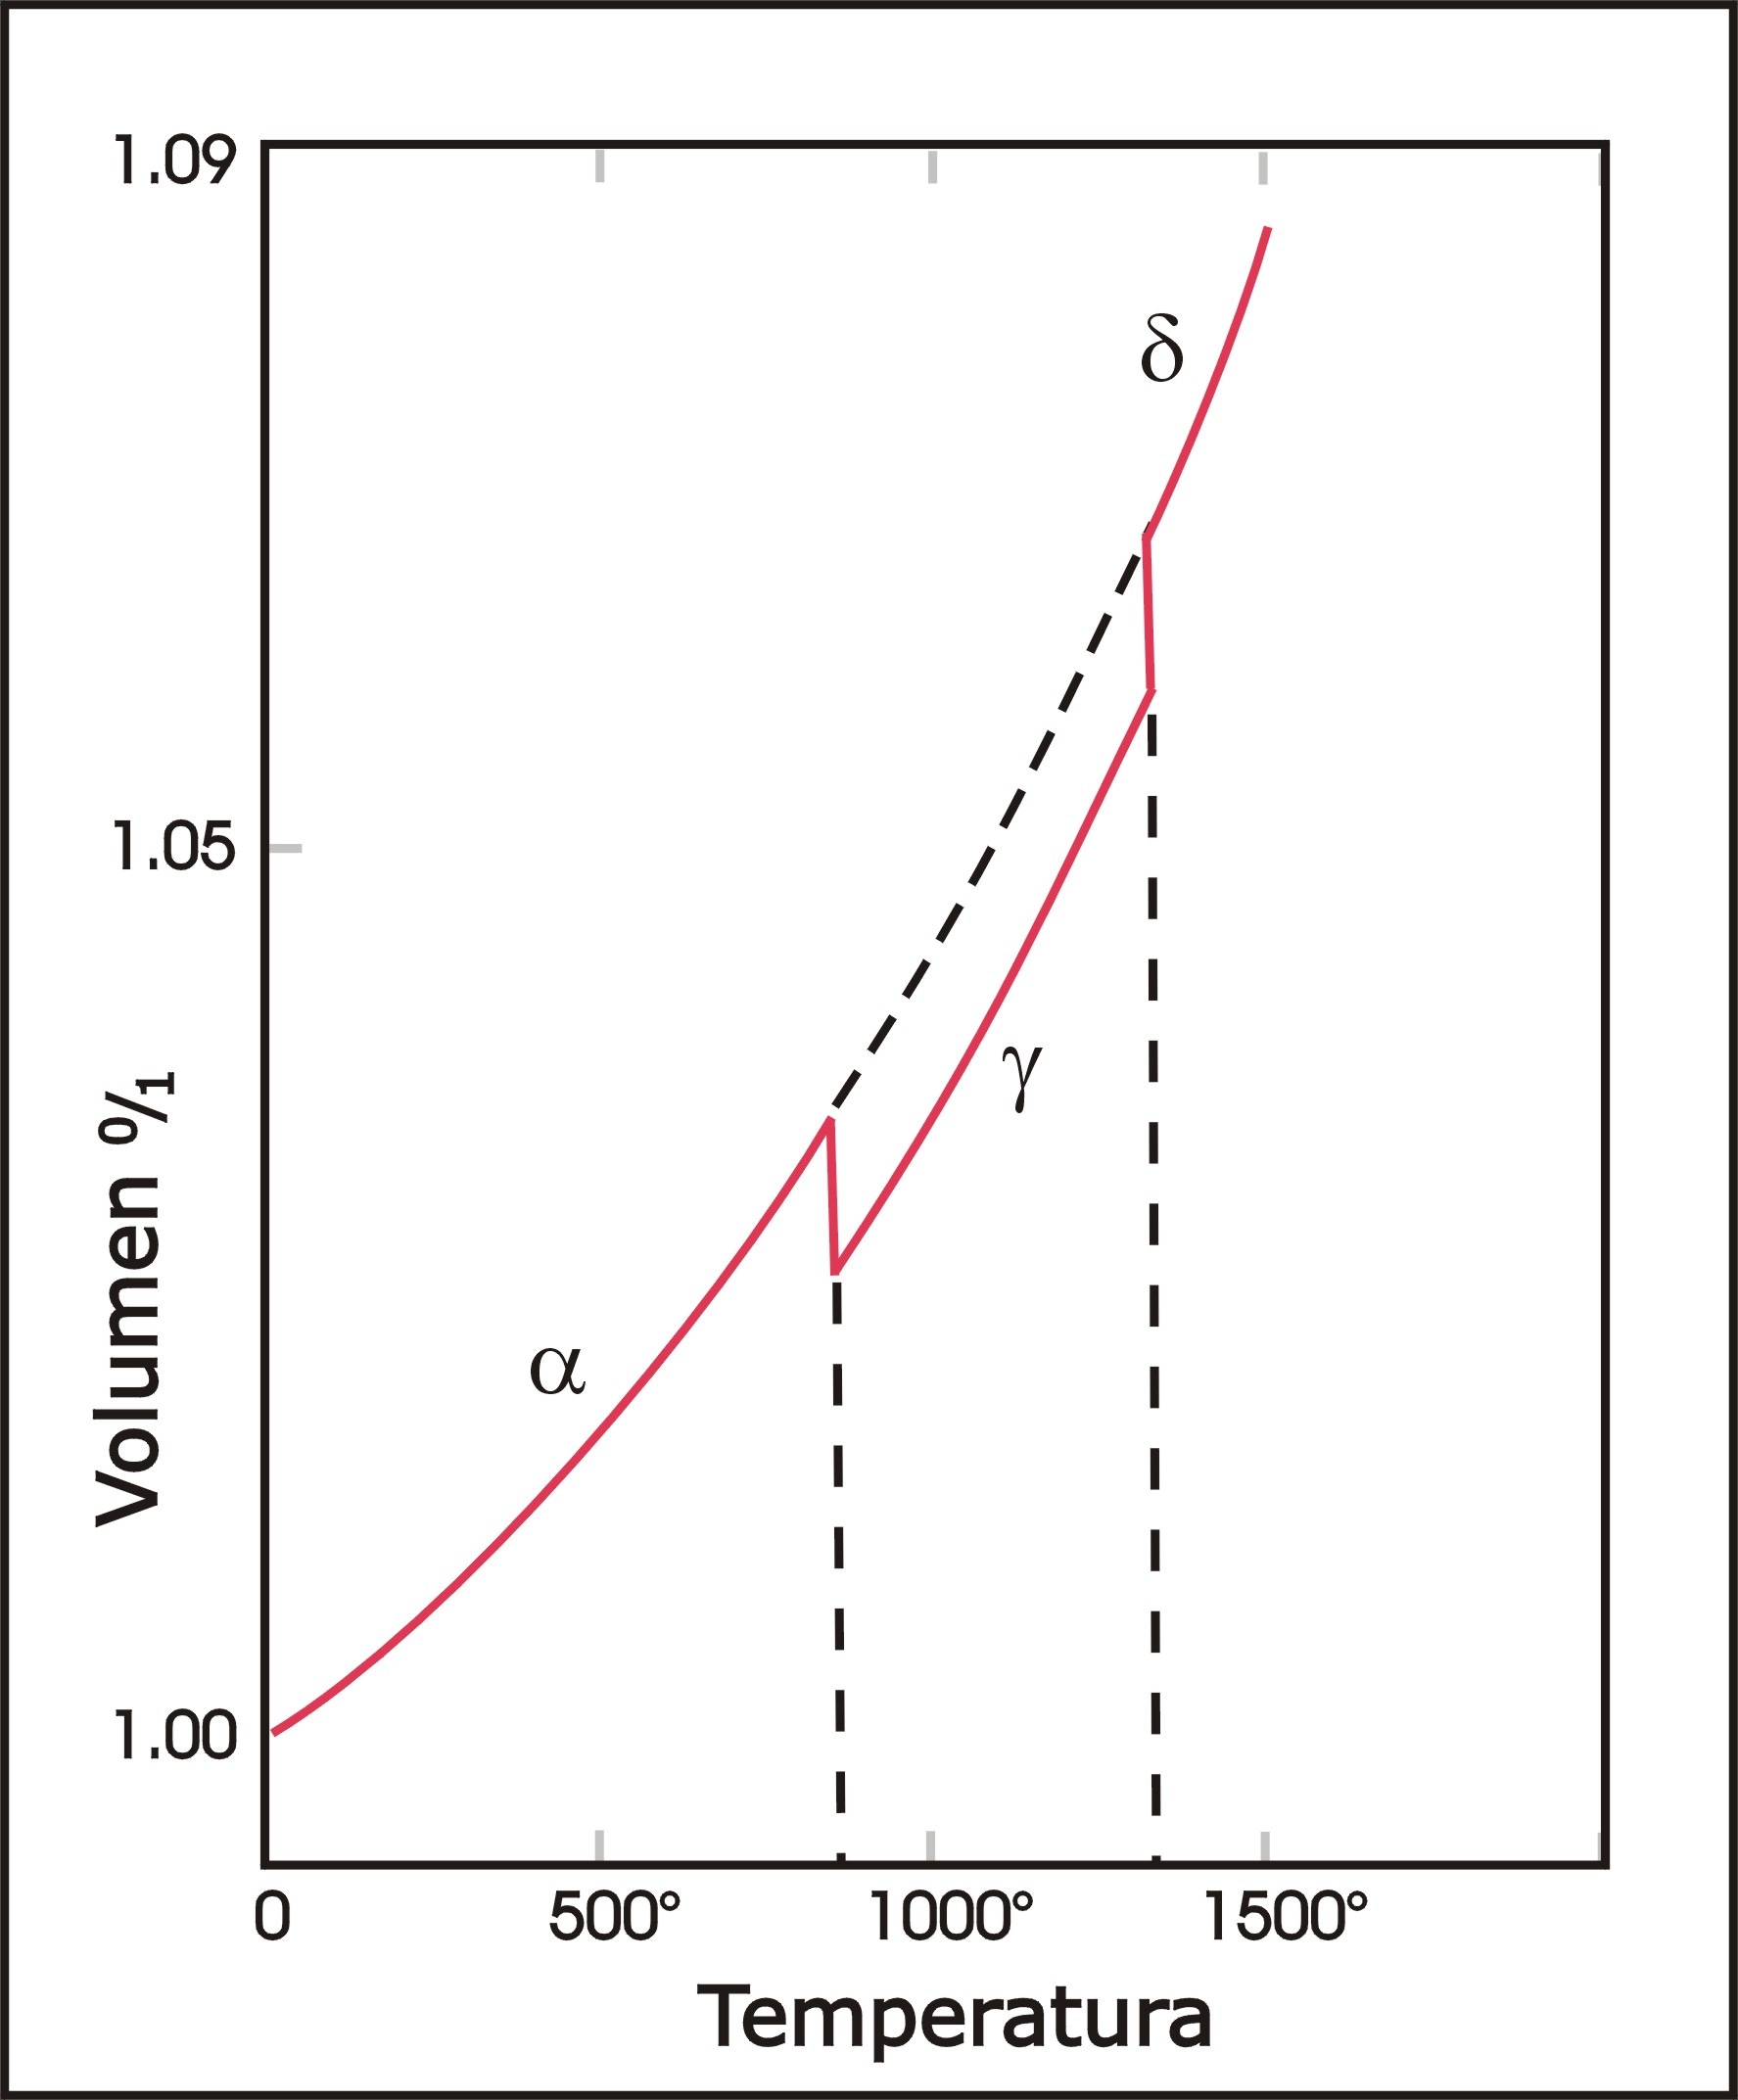
\includegraphics[width=0.6\textwidth]{./Figures/particularidadFe1}
	\caption{Densidades relativas $Fe\,\alpha-\gamma-\delta$}
	\label{fig:particularidadFe1}
\end{figure}

En general la fase estable a baja temperatura es la de menor energía interna o bien, la que tenga estructura más compacta. A temperatura altas el valor de la entropía y la temperatura son más importantes, dando posibilidad a
estructuras menos compactas.

El hierro puro tiene un comportamiento particular, la energía interna y la entropía por la presencia de la transformación de segundo orden (transformación paramagnética - ferromagnética) modifican esta situación. El
esquema de la figura \ref{fig:particularidadFe2} muestra los cambios en el calor especifico de cada una de las fases \citep{CpFe}.

\begin{figure}[H]
    \centering
    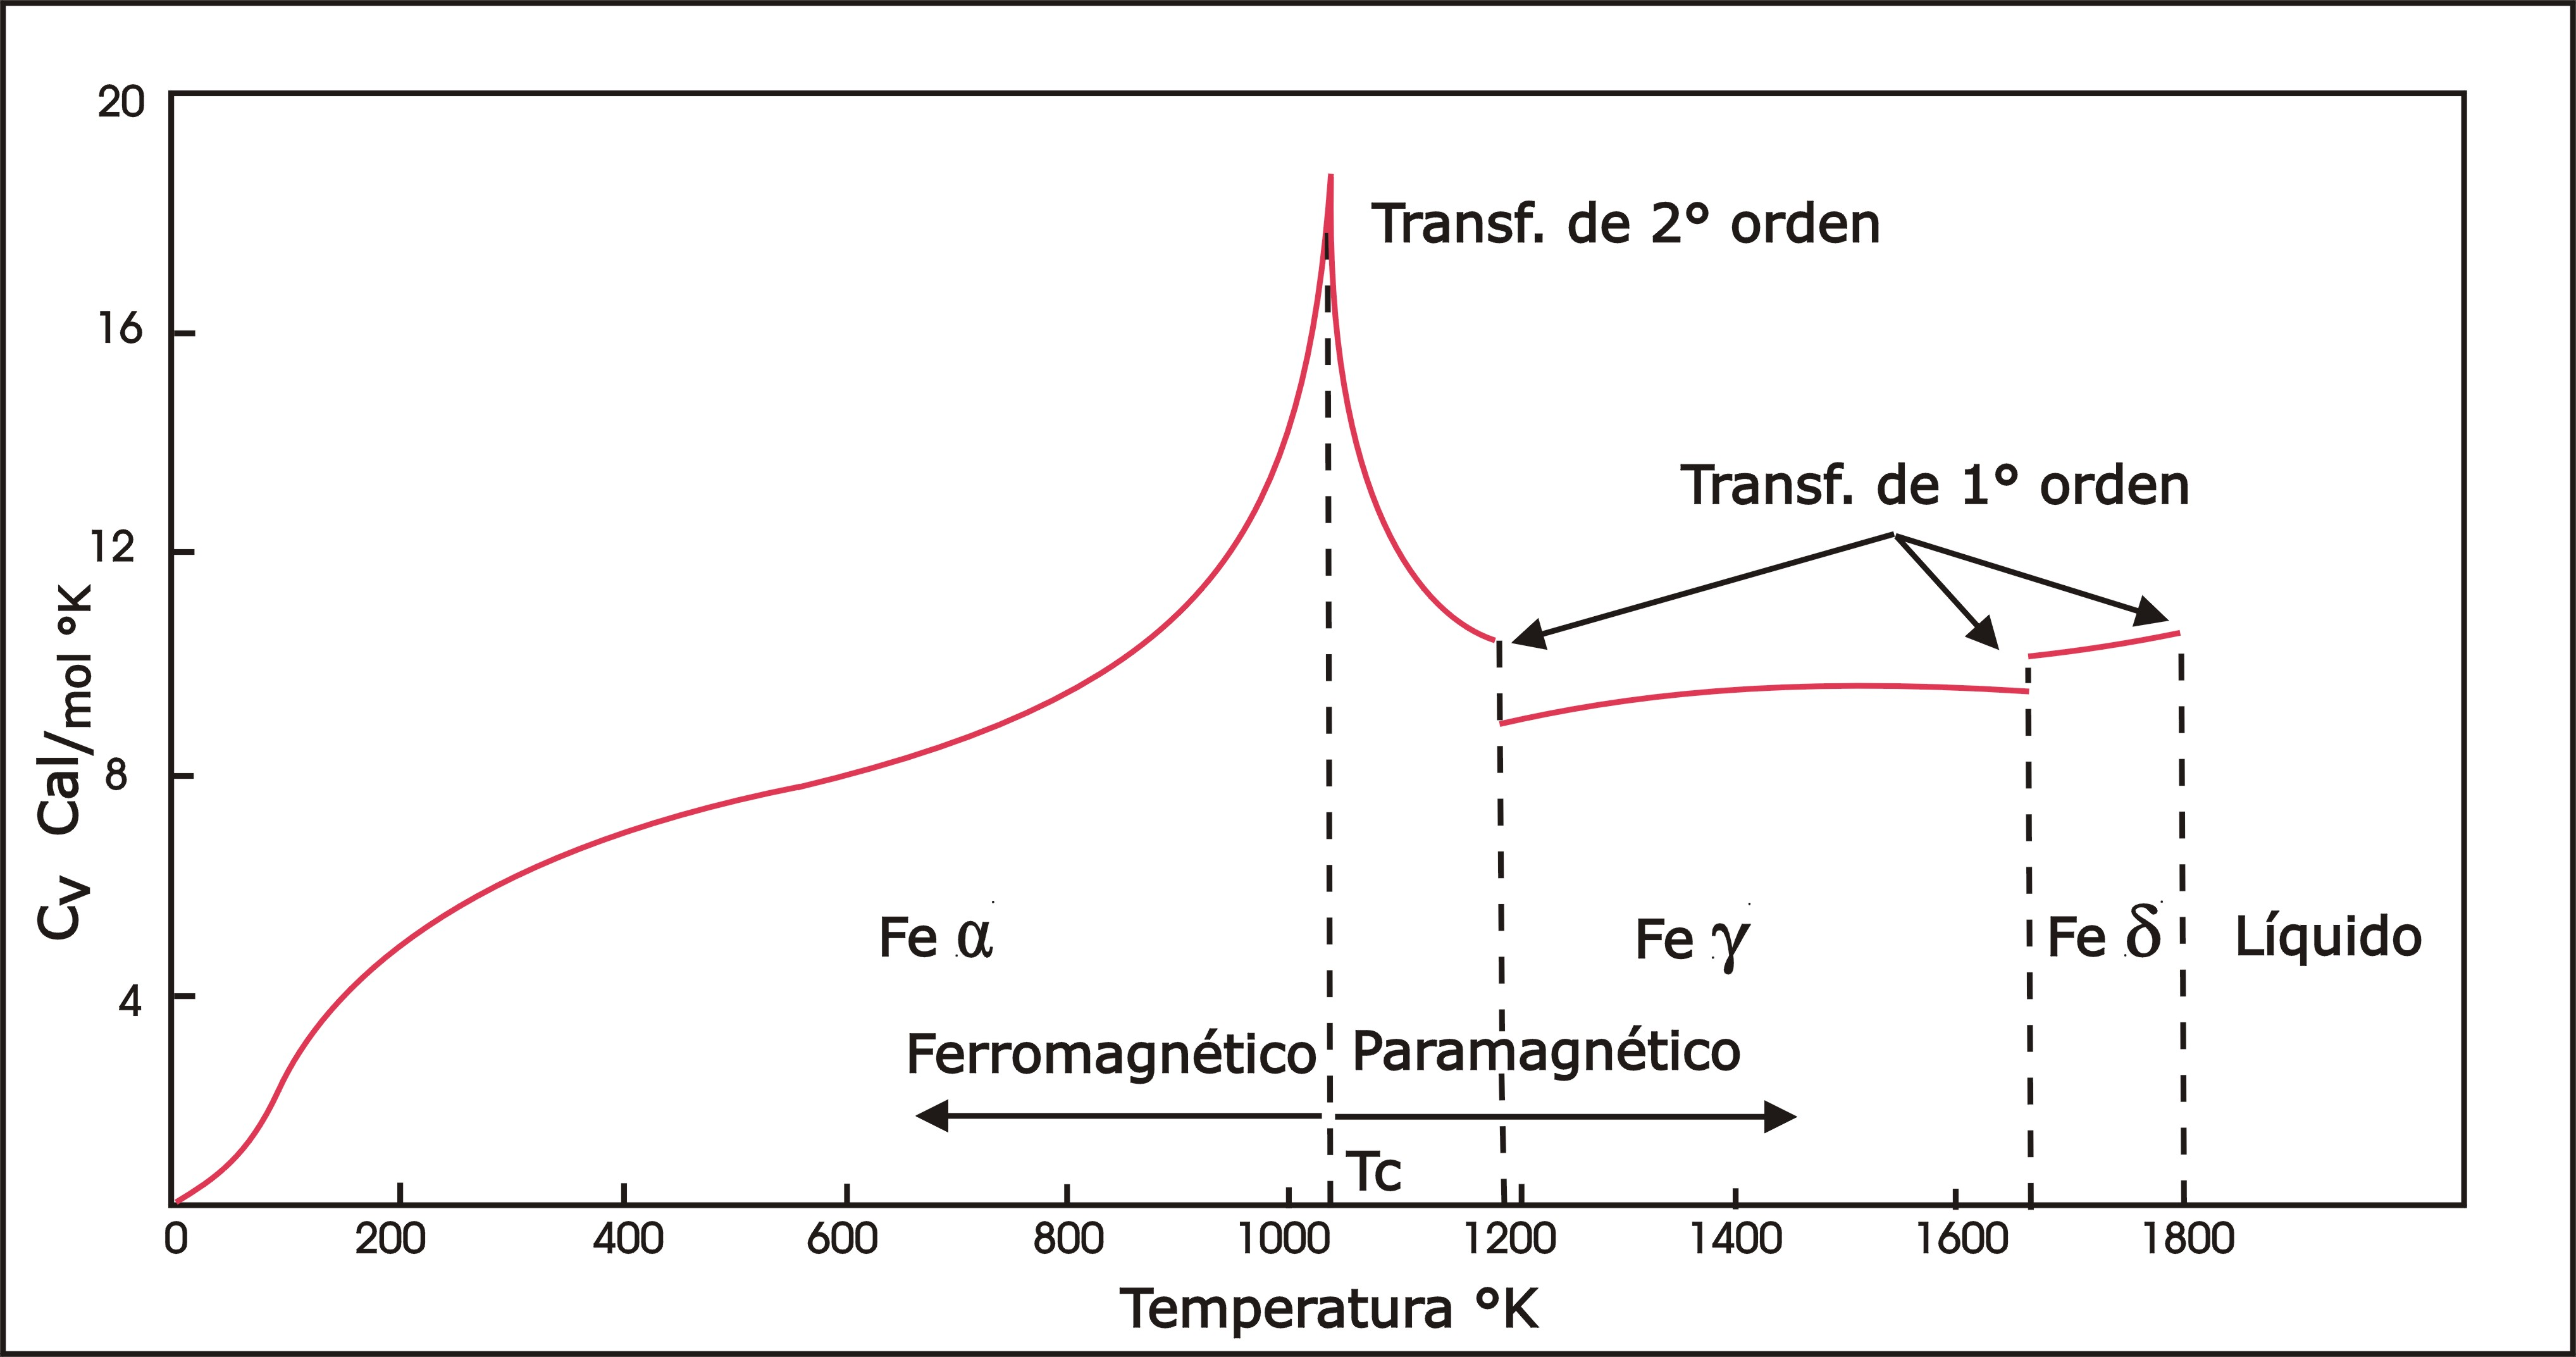
\includegraphics[width=1.0\textwidth]{./Figures/particularidadFe2}
	\caption{Transiciones de estado $Fe\,\alpha-\gamma-\delta$}
	\label{fig:particularidadFe2}
\end{figure}

\subsection{Ferromagnetismo en el hierro}

\begin{itemize}
	\item Para la explicación siguiente tomemos en particular el caso del hierro, la conclusión no solo será inherente a él.
	
	\item En la figura \ref{fig:particularidadFe2} se observa que por debajo de la temperatura $T_{C}$ llamada temperatura de Curie el hierro con la misma estructura cristalográfica pasa a ser ferromagnético. Esa misma temperatura
define una transformación, en estado sólido, de segundo orden, llamada también, de orden-desorden. Bajo ciertas circunstancias y con determinados elementos (en nuestro caso átomos) que constituyen un conjunto, el espacio determinado por los elementos se puede estructurar, ¿qué significa estructurar?, que se subdivide en celdas (zonas espaciales) que tienen características (propiedades) similares, apareciendo una estructura emergente que adquirió cierto orden. Para que el sistema se estructure los individuos que lo forman deben notar la presencia del otro, esto implicaría algún tipo de interacción entre ellos, por lo cual les convenga estructurarse. Este fenómeno requiere un tiempo que es característico del sistema.

	\item Por debajo de $T_{c}$ se genera una estructura llamado orden magnético que implica la existencia de zonas de varias distancias atómicas con momento magnético paralelo, llamados dominios magnéticos. Esto se genera espontáneamente sin que haya existido ninguna acción externa.
	
	\item Veamos que sucede por arriba de $T_{c}$: sabemos que cada átomo de hierro posee un momento magnético determinado por los electrones no apareados, luego debe existir una interacción entre ellos aparte de la que los mantiene unidos.
	
	\item También sabemos que las estructuras cristalinas de los sólidos metálicos son consistentes con una imagen de ellos como esferas duras empaquetadas y que la energía térmica está asociada con la vibración de estos en suposición de equilibrio. A mayor temperatura mayores el rango de oscilación, compitiendo con los momentos magnéticos que por arriba de $T_{c}$ no logran generar un orden magnético, por tanto el sólido no presenta un momento magnético total. Si se acerca un imán se logra un momento magnético.

	\item Al bajar la temperatura comienza a generarse un orden coincidiendo con las afirmaciones de \textbf{Gnedenko Kolmogoroff} que escribieron: los fenómenos aleatorios considerados en su acción colectiva a gran escala, crean una regularidad no aleatoria.

	\item Toda acción colectiva posee al menos un aspecto que es en el límite, regular y no aleatorio.
\end{itemize}


\section{Interacción de canje}


La interacción de canje fue descubierta independientemente por Heisenberg y Dirac en 1926 y está íntimamente relacionada con el del principio de exclusión de Pauli, 1925. Surge de forma natural al considerar la indistinguibilidad de algunas partículas. En mecánica clásica las partículas son distinguibles y se describen con la estadística de Maxwell Boltzmann en la mecánica cuántica no existe un procedimiento físico para distinguirlas o decir si una partícula observada en un instante es la misma que otra observada en un instante posterior. Esta circunstancia hace que el tratamiento cuántico adecuado de las partículas idénticas requiera la estadística Bose Einstein. El Ferromagnetismo es consecuencia del alineamiento de los espines de átomos adyacentess

Las fuerzas de canje dependen fundamentalmente de las distancias atómicas y no de posiciones atómicas la cristalinidad no es condición para el ferromagnetismo

La anisotropía magnética es la no homogeneidad de las propiedades magnéticas.

El ferromagnetismo no es particularidad de un tipo de estructura cristalina,
como vemos en la tabla. Lo que es característico de estos materiales es la presencia de capas $d$ o $f$ parcialmente llenas.


\subsection{Fuerza de canje:}

\begin{itemize}
	\item Tanto el diamagnetismo como el paramagnetismo se pudieron explicar, como fue visto anteriormente, pero no puede explicar el ferromagnetismo. Para que exista el ferromagnetismo debe existir algún tipo de fuerza que genere este ordenamiento.
	
	\item \textbf{Weiss} en 1907, antes de la aparición de la Mecánica Cuántica, sugirió la existencia de un ''campo molecular” responsable del ordenamiento. Era un explicación fenomenológica, puesto que no se la podía explicar analíticamente.
	
	\item Posteriormente \textbf{Frenkel} y \textbf{Heisemberg} demuestran que existe una interacción electrostática intensa entre los electrones que energéticamente favorece que los espines se ubiquen de manera paralela

	\item Esto se logro colocando en la ecuación de la energía, además del término clásico coulombiano, otro netamente cuántico que depende de la orientación mutua de los spines. Este término se lo llamó \textbf{energía de canje o de intercambio} representándolo con la letra $J_{ij}$. Dando una explicación a la propuesta de Weiss.

	\item El signo de $J_{ij}$ es fundamental para la explicación del ferromagnetismo.
	\begin{itemize}
	\item[1] En el caso de la molécula de hidrogeno $J_{ij<0}$, el estado de menor energía es aquel en el que los espines son antiparalelos $S=0$. 
	
	\item[2] En el caso de algunos sólidos $J_{ij}>0$ y los estados de menor energía son aquellos en los que el valor del espín S es máximo (reglas de Hund). 
	\end{itemize}
	
	
	\item $J_{ij}$ puede tomar valores positivos o negativos dependiendo del caso en particular.
	
	\item Energía total asociada será $E=-\sum_{ij}J_{ij}S_{i}S_{j}$
	
	\item Si $J_{ij}>0$ entonces $E$ es mínima si los $S$ son paralelos.
	
	\item Si $J_{ij}<0$ entonces $E$ es mínima si los $S$ son antiparalelos (moléculas).
	
	\item Esta conclusión aparentemente contradictoria, la explica Heisemberg (1928); diciendo que en la molécula de hidrógeno solo tenemos dos electrones y poca influencia del resto, mientras que en los sólidos, cada electrón atómico no es solo perturbado por otros electrones, sino por también por el efecto de todos los átomos vecinos, de manera que las contribuciones a la integral de canje $J_{ij}$ son variadas.

	\item El cálculo de $J_{ij}$ para un sistema de $n$ átomos es complejo. Se supone que la $J_{ij}$ es distinta de cero solo para los átomos $i$,$j$  vecinos y próximos de la red, mientras que para los lejanos $J_{ij}\rightarrow0$ , luego $J_{ij}=J$ 
 	
\end{itemize}

En la figura \ref{fig:energíaDeCanje} se observa que tienen energía de canje positiva el $Fe$, $Co$, $Ni$. Los tres son ferromagnéticos mientras que $Mn$ tiene energía de canje negativa, o sea, sus espines son antiparalelos dando origen a los materiales antiferromagnéticos


\begin{figure}[H]
    \centering
    \includegraphics[width=0.6\textwidth]{./Figures/energíaDeCanje}
	\caption{Energía de canje para distintos elementos}
	\label{fig:energíaDeCanje}
\end{figure}

\section{Antiferromagnéticos y Ferrimagnéticos}

\begin{itemize}
	\item Cuando los átomos solapan sus funciones de onda, esto es, cuando están relativamente próximos, interactúan alineando sus spines si $J>0$ da origen al ferromagnetismo. Por el contrario si $J<0$  el material es antiferromagnético con magnetización neta cero. Las espines de los átomos adyacentes son opuestos. En este caso también a una temperatura, llamada de \textbf{Neel} se vuelven paramagnéticos. Ejemplos de estos materiales son $MnF$, $MnO$, $FeO$.
	
	\begin{figure}[H]
    %\centering
    \hspace{4.0cm}
    \includegraphics[width=0.5\textwidth]{./Figures/antiferromagnético}
	%\caption{}
	\label{fig:antiferromagnético}
	\end{figure}
	
	
	\item Hay una situación intermedia entre ferromagnéticos y los antiferromagnéticos cuando hay varios elementos con diferente número de electrones desapareados. En este caso aunque se dispongan de forma antiparalela el momento magnético resultante es diferente de cero ya que un elemento tienen mayor momento magnético que otro, estos compuestos se conocen como ferrimagnéticos.
	
	
	\begin{figure}[H]
    %\centering
    \hspace{4.0cm}
    \includegraphics[width=0.5\textwidth]{./Figures/ferrimagnético}
	%\caption{}
	\label{fig:ferrimagnético}
	\end{figure}
	
	
	\item De otro modo si tenemos una sustancia formada por dos subredes ferromagnéticas de momentos ferromagnéticos antiparalelos tenemos un material ferrimagnético.
	
	\item El ejemplo más común es la ferrita pudiente tener un momento magnético importante, la primera ferrita que se conoció fue la magnetita $Fe_{3}O_{4}$ ya que tiene la posibilidad de presentarse magnetizada de un modo natural. En los años 50 se observó que este tipo de óxidos presentan una elevada resistividad eléctrica, propiedad que evita las corrientes parásitas que implican pérdidas de energía cuando se los utiliza como núcleos . Resultan, por tanto, útiles en dispositivos que trabajan con elevadas frecuencias.

\end{itemize}

\subsection{Suceptibilidad y Temperatura}

En la figura \ref{fig:suceptibilidades} se representa la variación de la $\chi$ susceptibilidad
magnética para varios ordenamientos magnéticos, recordando que: $\chi=\frac{M}{H}$ donde {M} es la magnetización del material o sea la respuesta del material al campo $H$. Observamos que salvo los diamagnéticos los
otros ordenamientos disminuyen $\chi$ con el aumento de la temperatura.
También vemos que después de las temperaturas $T_{N}$ o $T_{C}$ el
comportamiento es como el de los paramagnéticos. ¿Por qué?.

\begin{figure}[H]
    \centering
    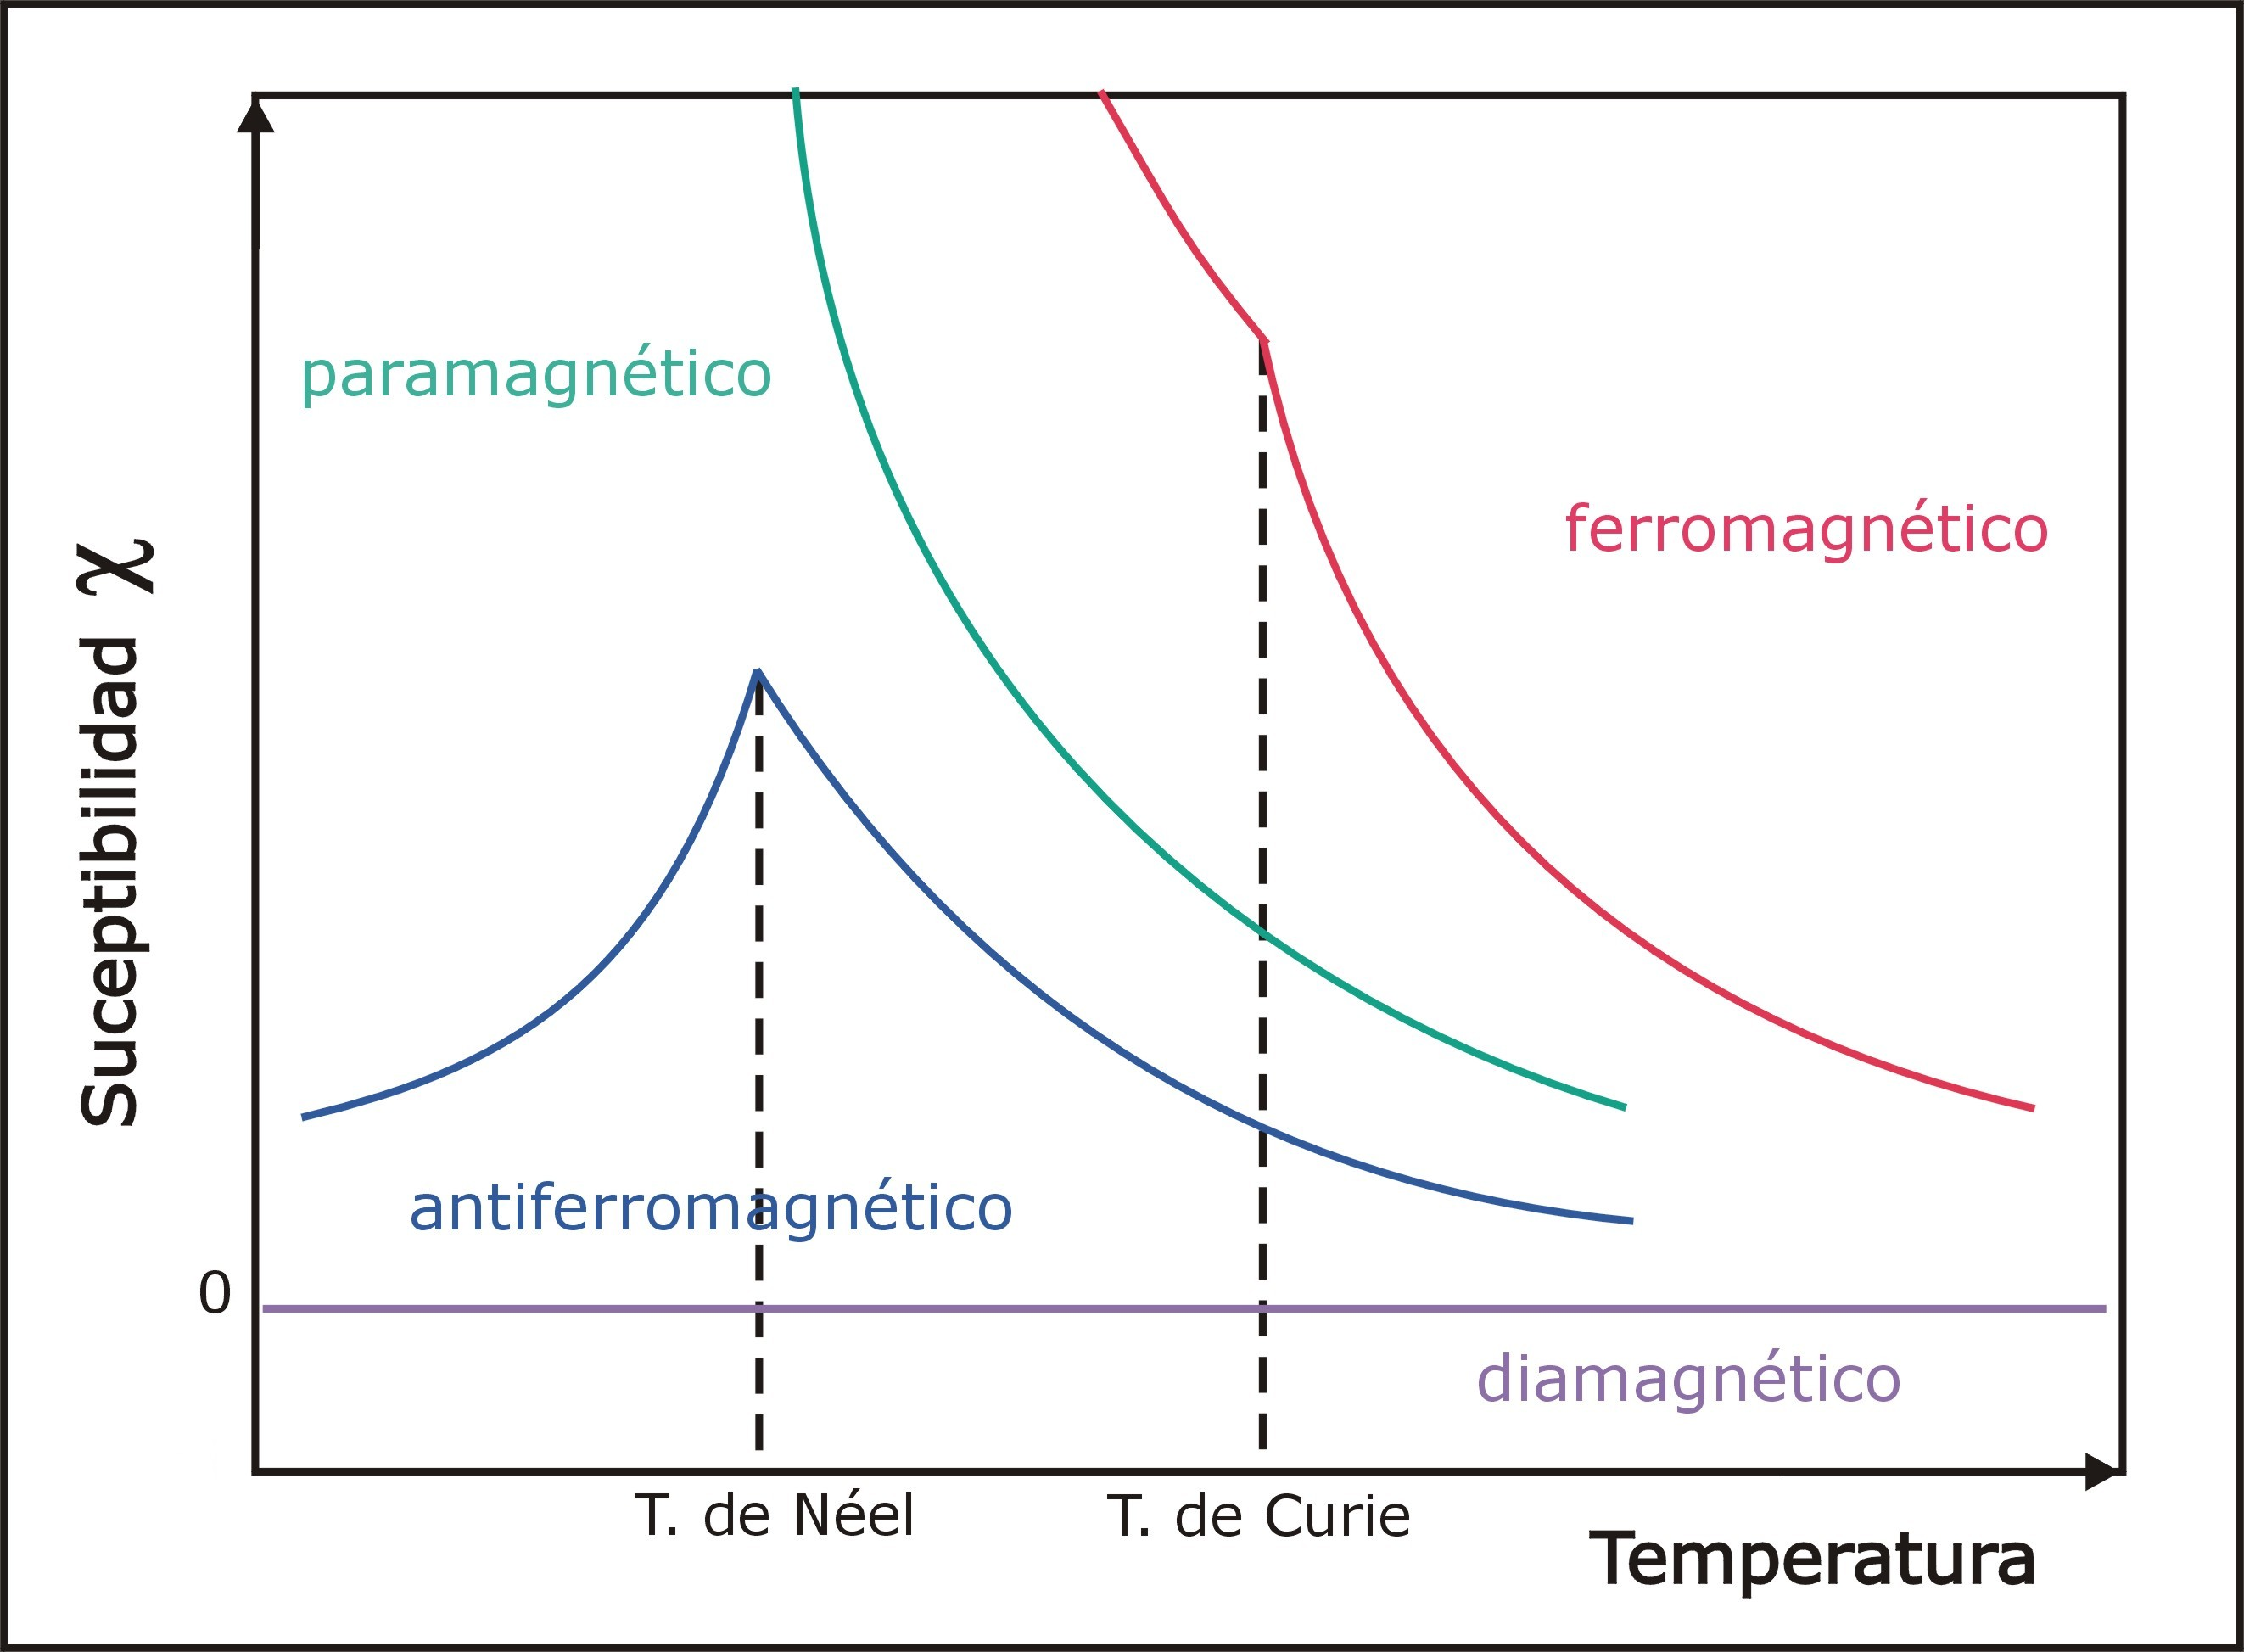
\includegraphics[width=0.9\textwidth]{./Figures/suceptibilidades}
	\caption{Susceptibilidades y temperaturas de transición}
	\label{fig:suceptibilidades}
\end{figure}

\subsection{Canje y Supercanje}

\begin{itemize}
	\item Vimos que los átomos con capas $d$ o $f$ incompletas, que interactúan formando una estructura ferromagnética o antiferromagnética, deben estar próximos uno del otro. Esta interacción se llama de canje directo.
	
\begin{figure}[H]
    \centering
    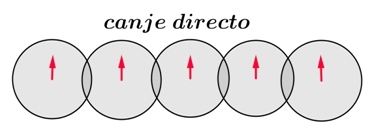
\includegraphics[width=0.5\textwidth]{./Figures/canjeDirecto}
	%\caption{Elementos de transición interna}
	\label{fig:canjeDirecto}
\end{figure}		
	
	
	\item Pero en muchos compuestos químicos los iones magnéticos esta separados por otro no magnético (diamagnético), en estos casos la interacción es realizada por los electrones del ion no magnético y es llamada de supercanje o superintercambio. Este mecanismo fue propuesto en 1934.
	

\begin{figure}[H]
    \centering
    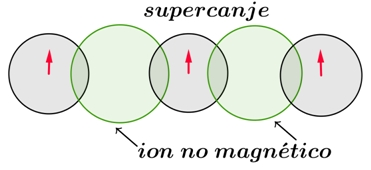
\includegraphics[width=0.5\textwidth]{./Figures/canjeSupercanje}
	%\caption{Elementos de transición interna}
	\label{fig:canjeSupercanje}
\end{figure}	
	
	
	\item Un caso típico de supercanje es el $MnO$ que se analiza seguidamente.
\end{itemize}

\subsection{Desdoblamiento del campo cristalino}

\textbf{Posiciones octaédrica y tetraédrica:}

Cuando tenemos átomos iguales que se unen para establecer un enlace metálico, se forman los empaquetamientos densos que se describen como un agradado de esferas duras. Estas esferas constituyen principalmente dos tipos de estructuras cristalinas compactas; cubica centrada en las caras (FCC) y hexagonal (HCP).

Existen empaquetados de orden superior que no comentaremos, Estas estructuras poseen una característica muy importante, al formarse el sólido quedan huecos entre los átomos que se llaman intersticios, los hay de varios tipos, pero aquí solo estudiaremos dos: tetraédrica (coordinación 4) y octaédrica (coordinación 6).

\begin{figure}[H]
    \centering
    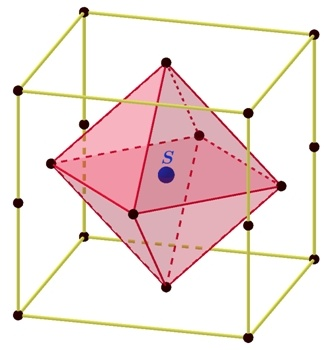
\includegraphics[width=0.6\textwidth]{./Figures/MnOctaedrica}
	\caption{Mn S posición octaédrica.}
	\label{fig:MnOctaedrica}
\end{figure}

\begin{figure}[H]
    \centering
    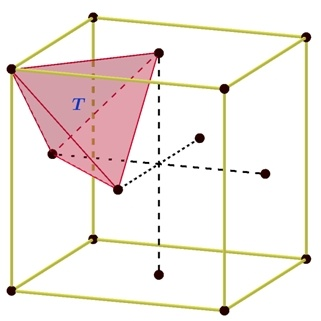
\includegraphics[width=0.6\textwidth]{./Figures/MnTetragonal}
	\caption{Mn T posición tetraédrica.}
	\label{fig:MnTetraedrica}
\end{figure}

\begin{itemize}
	\item En el esquema octaédrico, anterior mente mostrado, el lugar designado con S (octaédrico) es ocupado por un átomo de la misma especie. Sin embargo es común que el sitio octaédrico sea ocupado por catión metálico, que se enlaza a otras entidades moleculares que lo rodean llamadas ligandos.
	
	\item Recordemos que los elementos de transición tienen 5 orbitales $d$ con diferente orientación en el espacio. Si el núcleo se encuentra en el centro de coordenadas, los tres orbitales $d_{xz}$, $d_{xy}$ y $d_{yz}$ tienen cuatro lóbulos cada uno dirigido entre los ejes de coordenadas, los dos restantes $3d_{z}2$, $3d_{x}2-_{y}2$, tienen sus lóbulos dirigidos a lo largo de los ejes. En un átomo aislado o campo esférico estos cinco orbitales tienen la misma energía (degenerados). No sucede lo mismo en un sólido.

	\item Observemos que cada ion metálico está rodeado por seis Iones ligantes. Estos modifican los cinco orbitales (degenerados) $d$ del metal central (en el caso de los elementos de transición), alterando sus energías. Luego los cinco orbitales $d$ se separan en dos grupos de diferente energía. El acercamiento de los ligandos perturban los orbitales $d$, cambiando su estado de degeneración.

	\item Se originarán diferentes tipos de estructuras básicas si están ocupados total o parcialmente por cationes.
	
	\item Según su carácter los ligantes pueden ejercer una interacción (campo cristalino) fuerte o débil. Esto es muy importante si hay dos estados próximos de energía, lo que se conoce como estados de baja y alta espín. Si es posible pasar de uno a otro por cambios en la presión ,temperatura o iluminación tenemos un sistema de dos fases magnéticas. La teoría del campo cristalino ha tenido éxito en la explicación de varios fenómenos, color, propiedades magnéticas, etc. 

\end{itemize}

En el caso del campo octaédrico los orbitales de los ligandos se extienden casi hasta los orbitales $d_{z}2$ y $d_{x}2-_{y}2$, pudiendo tener contacto directo entre ellos.


\begin{figure}[H]
    \centering
    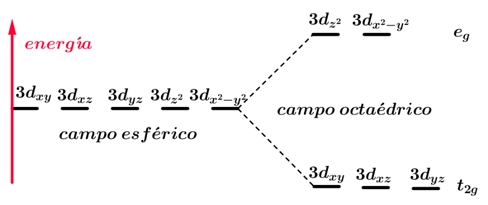
\includegraphics[width=0.8\textwidth]{./Figures/campoEsferico1}
	\caption{Campo esferico - octaédrico}
	\label{fig:campoEsferico1}
\end{figure}


\begin{figure}[H]
    \centering
    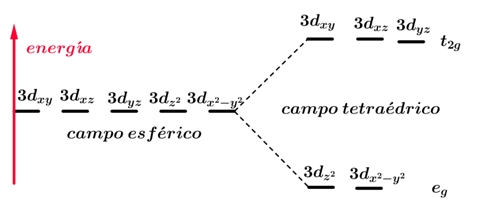
\includegraphics[width=0.8\textwidth]{./Figures/campoEsferico2}
	\caption{Campo esferico - tetraédrico}
	\label{fig:campoEsferico2}
\end{figure}

Esto produce la repulsión electrón-electrón deformando los orbitales, con el consiguiente aumento de la energía de los orbitales $d_{x}2$ y $d_{x}2-_{y}2$. No pasa lo mismo con los otros tres orbitales $d_{xy}$, $d_{yz}$ y $d_{xz}$. A esta partición de los orbitales cuando el campo no es esférico se lo conoce como desdoblamiento del Campo cristalino. Esta diferencia de energía suele simbolizarse con la letra $\Delta$ . Los orbitales $d$ pueden ser llenados de varias maneras. Si la energía $\Delta$ es menor que la energía de canje $J$ el llenado de los orbitales se hace de acuerdo a la regla de Hund, luego el espín del sistema debe ser máximo.

%\section{Antiferromagnéticos y Ferrimagnéticos}

Vemos en la estructura del $MnO$, material antiferromagnético, que se trata de un material cerámico de características iónicas $Mn^{2+}$ y $O^{2-}$.

\begin{equation}
\begin{aligned}
	Mn: [Ar]3d^{5}4s^{2}\rightarrow Mn^{2+}: [Ar]3d^{5}4s^{0}  \\
	O: [He]2s^{2}2p^{4}\rightarrow O^{2-}: [He]2s^{2}2p^{6}
\end{aligned}
\end{equation}

El oxigeno al ionizarse completa sus orbitales por lo que el momento magnético es nulo. Por el contrario el $Mn$ tiene electrones desapareados y por tanto un momento magnético.

\begin{figure}[H]
    \centering
    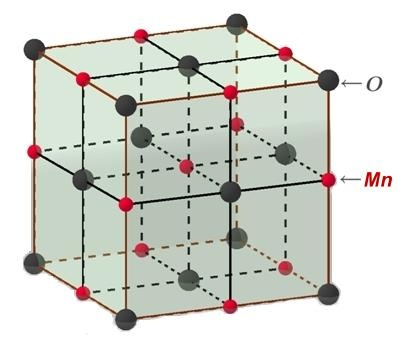
\includegraphics[width=0.6\textwidth]{./Figures/FerroAntiferri2}
	\caption{Antiferrimagnetismo $MnO$}
	\label{fig:FerroAntiferri2}
\end{figure}


Analicemos la configuración electrónica del $[Mn^{2+}]$: $[Ar]3d^{5}4s^{0}$: Los niveles $3d$ del átomo de $Mn$ en su estado normal tienen igual energía. Esta estructura puede pensarse como formada por dos redes cúbicas centradas en las caras interpenetradas, una formada por los $Mn$ y la otra por los $O$, estos últimos de mayor tamaño. Ver figura \ref{fig:FerroAntiferri3}:

\begin{figure}[H]
    \centering
    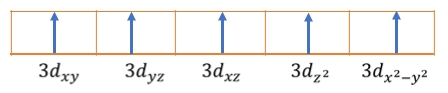
\includegraphics[width=0.8\textwidth]{./Figures/FerroAntiferri3}
	\caption{Alineacion de los niveles $3d$}
	\label{fig:FerroAntiferri3}
\end{figure}


\subsection{Estructura del MnO, campo cristalino}

Observamos en esta estructura cubica, que los huecos octaédricos están todos ocupados por iones de $Mn$.

La red es una alternancia de dos estructuras cada una de ellas contiene iones de un solo signo. Es una alternancia de iones a lo largo de las direcciones cristalográficas $[100]$ ,$[010]$ y $[001]$.

En la figura \ref{fig:estructuraMnO} vemos que cada ion de $Mn$ está rodeado por 6 Iones de $O$ llamados ligantes, estos modifican los cinco orbitales (degenerados) $d$ del metal central, alterando sus energías. Luego los cinco orbitales $d$ se separan en dos grupos de diferente energía, como vimos anteriormente.

\begin{figure}[H]
    \centering
    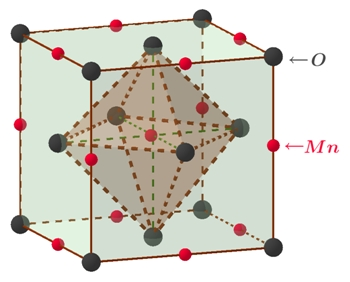
\includegraphics[width=0.6\textwidth]{./Figures/estructuraMnO}
	\caption{Estructura del $MnO$}
	\label{fig:estructuraMnO}
\end{figure}

El llenado de los orbitales será diferente dependiendo de que el campo cristalino sea fuerte o débil. Es claro que si el campo cristalino es débil o muy débil no debería haber degeneración y si la hay el llenado de los orbitales será como lo predice las reglas de Hund. No se requiere de mucha energía para que un electrón de los orbitales inferiores pase a los orbitales superiores. Por el contrario, cuando el campo cristalino es importante, se requiere más energía para llevar dos electrones de los orbitales inferiores a los superiores y es más conveniente energéticamente aparearlos con otro electrón de la órbita inferior.

En la figura \ref{fig:estructuraMnO2} siguiente se observa las distribuciones de $Mn$ (rojo) y $O$ (negro) en la estructura cristalina, mientras que en la figura \ref{fig:estructuraMnO3} se representa solo el plano (azul) del cubo. También se ve que los dos $Mn$ que se encuentran a la distancia (a) interactúan y tienen la misma dirección del momento magnético por el contrario los que se encuentran a una distancia mayor (b) es opuesto.


\begin{figure}[H]
    \centering
    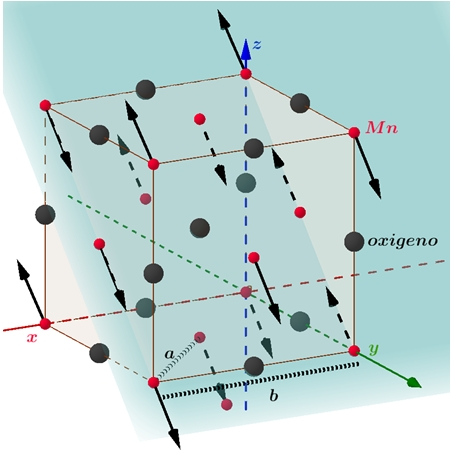
\includegraphics[width=0.6\textwidth]{./Figures/estructuraMnO2}
	\caption{Elementos de transición interna}
	\label{fig:estructuraMnO2}
\end{figure}


\begin{figure}[H]
    \centering
    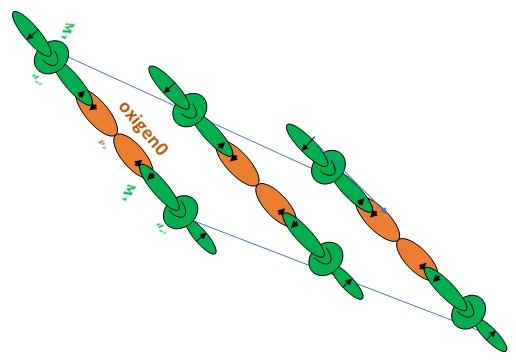
\includegraphics[width=0.6\textwidth]{./Figures/estructuraMnO3}
	\caption{Elementos de transición interna}
	\label{fig:estructuraMnO3}
\end{figure}

En la figura \ref{fig:campoDebil} vemos que si el campo es débil se distribuyen los electrones de acuerdo a Hund, mientras que si el campo cristalino es fuerte figura \ref{fig:campoFuerte} es preferible aparear dos electrones y no llevarlos al orbital superior.

\begin{figure}[H]
    \centering
    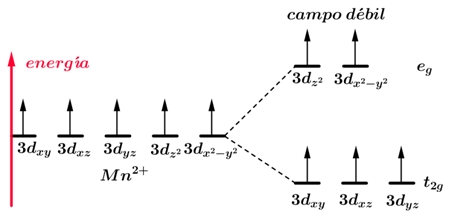
\includegraphics[width=0.8\textwidth]{./Figures/campoDebil}
	\caption{Campo débil}
	\label{fig:campoDebil}
\end{figure}

Comportamientos similares se observan en los distintos elementos de transición, por ejemplo en el $Fe^{3+}$ que también es del tipo $d^{5}$, similarmente con el $FE^{2+}$ y el $Co^{3+}$ que son del tipo $d^{6}$, etc.

\begin{figure}[H]
    \centering
    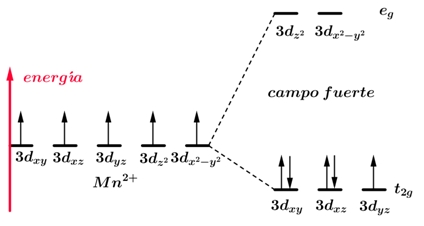
\includegraphics[width=0.8\textwidth]{./Figures/campoFuerte}
	\caption{Campo fuerte}
	\label{fig:campoFuerte}
\end{figure}

Fue posible establecer un orden relativo entre algunos ligandos que indican la fortaleza del campo cristalino por ellos generados. Como se indica en la figura \ref{fig:campoCristalino}.

\begin{figure}[H]
    \centering
    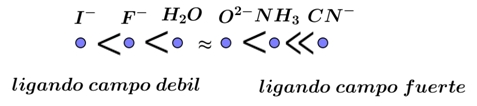
\includegraphics[width=0.6\textwidth]{./Figures/campoCristalino}
	\caption{Campo cristalino}
	\label{fig:campoCristalino}
\end{figure}


\subsection{Low espín y High espín}

Vemos en la figura \ref{fig:lowSpinHighSpin} los elementos en rojo, que pueden tener low o high espín en posiciones octaédricas.

\begin{figure}[H]
    \centering
    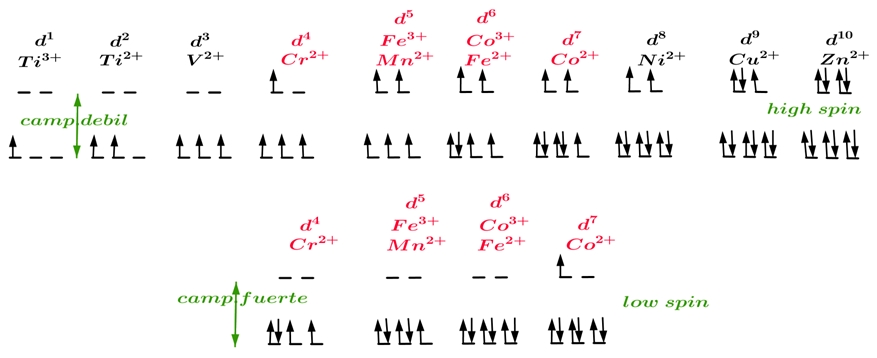
\includegraphics[width=1.0\textwidth]{./Figures/lowSpinHighSpin}
	\caption{Posiciones de low espín y High espín}
	\label{fig:lowSpinHighSpin}
\end{figure}

Algunas sustancias pueden exhibir transición de espín inducida térmicamente, conocida como \textit{crossover} de espín, dependiendo de la naturaleza del ligando. La transición de espín en tales compuestos también ocurre bajo presión e irradiación con luz. Los estados obtenidos tienen diferentes propiedades magnéticas y ópticas, con posibles aplicaciones como interruptores o memorias.

El esquema anterior mostraba los elemento en posición octaédrica, de esa manera, se trato el caso del $MnO$. El otro elemento que es de interés es el hierro por tal razón se agrega el $Fe^{3+}$ y el $Fe^{2+}$ en sitios
tetraédricos.

\begin{figure}[H]
    \centering
    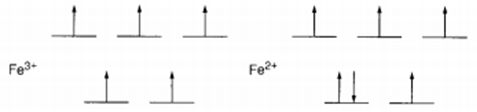
\includegraphics[width=0.6\textwidth]{./Figures/Fe3Fe2}
	\caption{Posiciones de low espín y High espín}
	\label{fig:Fe3Fe2}
\end{figure}

\subsubsection{Caso del hierro, Magnetita}

\begin{itemize}
	\item Veamos con un poco mas de detalle el caso del hierro, los estados de oxidación más comunes son $Fe^{2+}$ y $Fe^{3+}$, mientras el átomo neutro, como ya vimos, tiene la configuración electrónica $[Ar]3d^{6}4s^{2}$, y los iones las siguientes:
	\begin{equation}
	\begin{aligned}
		Fe: [Ar]3d^{6}4s^{2}\rightarrow Fe^{2+}: [Ar]3d^{6}4s^{0}  \\
		Fe: [Ar]3d^{6}4s^{2}\rightarrow Fe^{3+}: [Ar]3d^{5}4s^{0}
	\end{aligned}
	\end{equation}
	
	\item La magnetita se conoce como imán desde la antigüedad ($Fe_{3}O_{4}$), fue muy estudiada en la década de 1940.
	
	\item La magnetita pertenece al grupo de la espinela, su formula puede ser escrita como $MFe_{3}O_{4}$ donde $M$ es un catión divalente $M_{2+}$, cristaliza en una estructura cubica compacta, es un cerámico y se los fabrica por sinterizado. Los intersticios tetraédricos (A) y octaédricos (B) son ocupados por los cationes $M^{2+}$ y $Fe^{3+}$, pudiendo también ser $Zn^{2+}$, $Fe^{2+}$, $Mg^{2+}$, $Cd^{2+}$, etc. En general hay dos tipos de espinelas la normal y la inversa, la figura \ref{fig:espinela} las ilustra:
	
\begin{figure}[H]
    \centering
    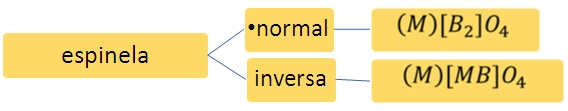
\includegraphics[width=0.6\textwidth]{./Figures/espinela}
	\caption{Espinelas Nomal e inversa}
	\label{fig:espinela}
\end{figure}

	\item Dando lugar a la representación $M[B_{2}]O_{4}$ donde ( ) indica posición tetraédrica y [ ] posición octaédrica. La magnetita es una espinela inversa luego la podemos escribir ${(Fe^{2+})[Fe^{2+}Fe^{3+}]O_{4}}$ lo que indica que tanto $Fe^{2+}$ como $Fe^{3+}$ se encuentran en posiciones octaédricas, como se observa en la figura \ref{fig:FeComplejo}.

En la figura \ref{fig:tablaDeOxidos} se muestran las propiedades magnéticas y estructurales de los oxido de $Fe$, con $M_{S}$: magnetización de saturación, $K$: constante de anisotropía magnética	
	
\begin{figure}[H]
    \centering
    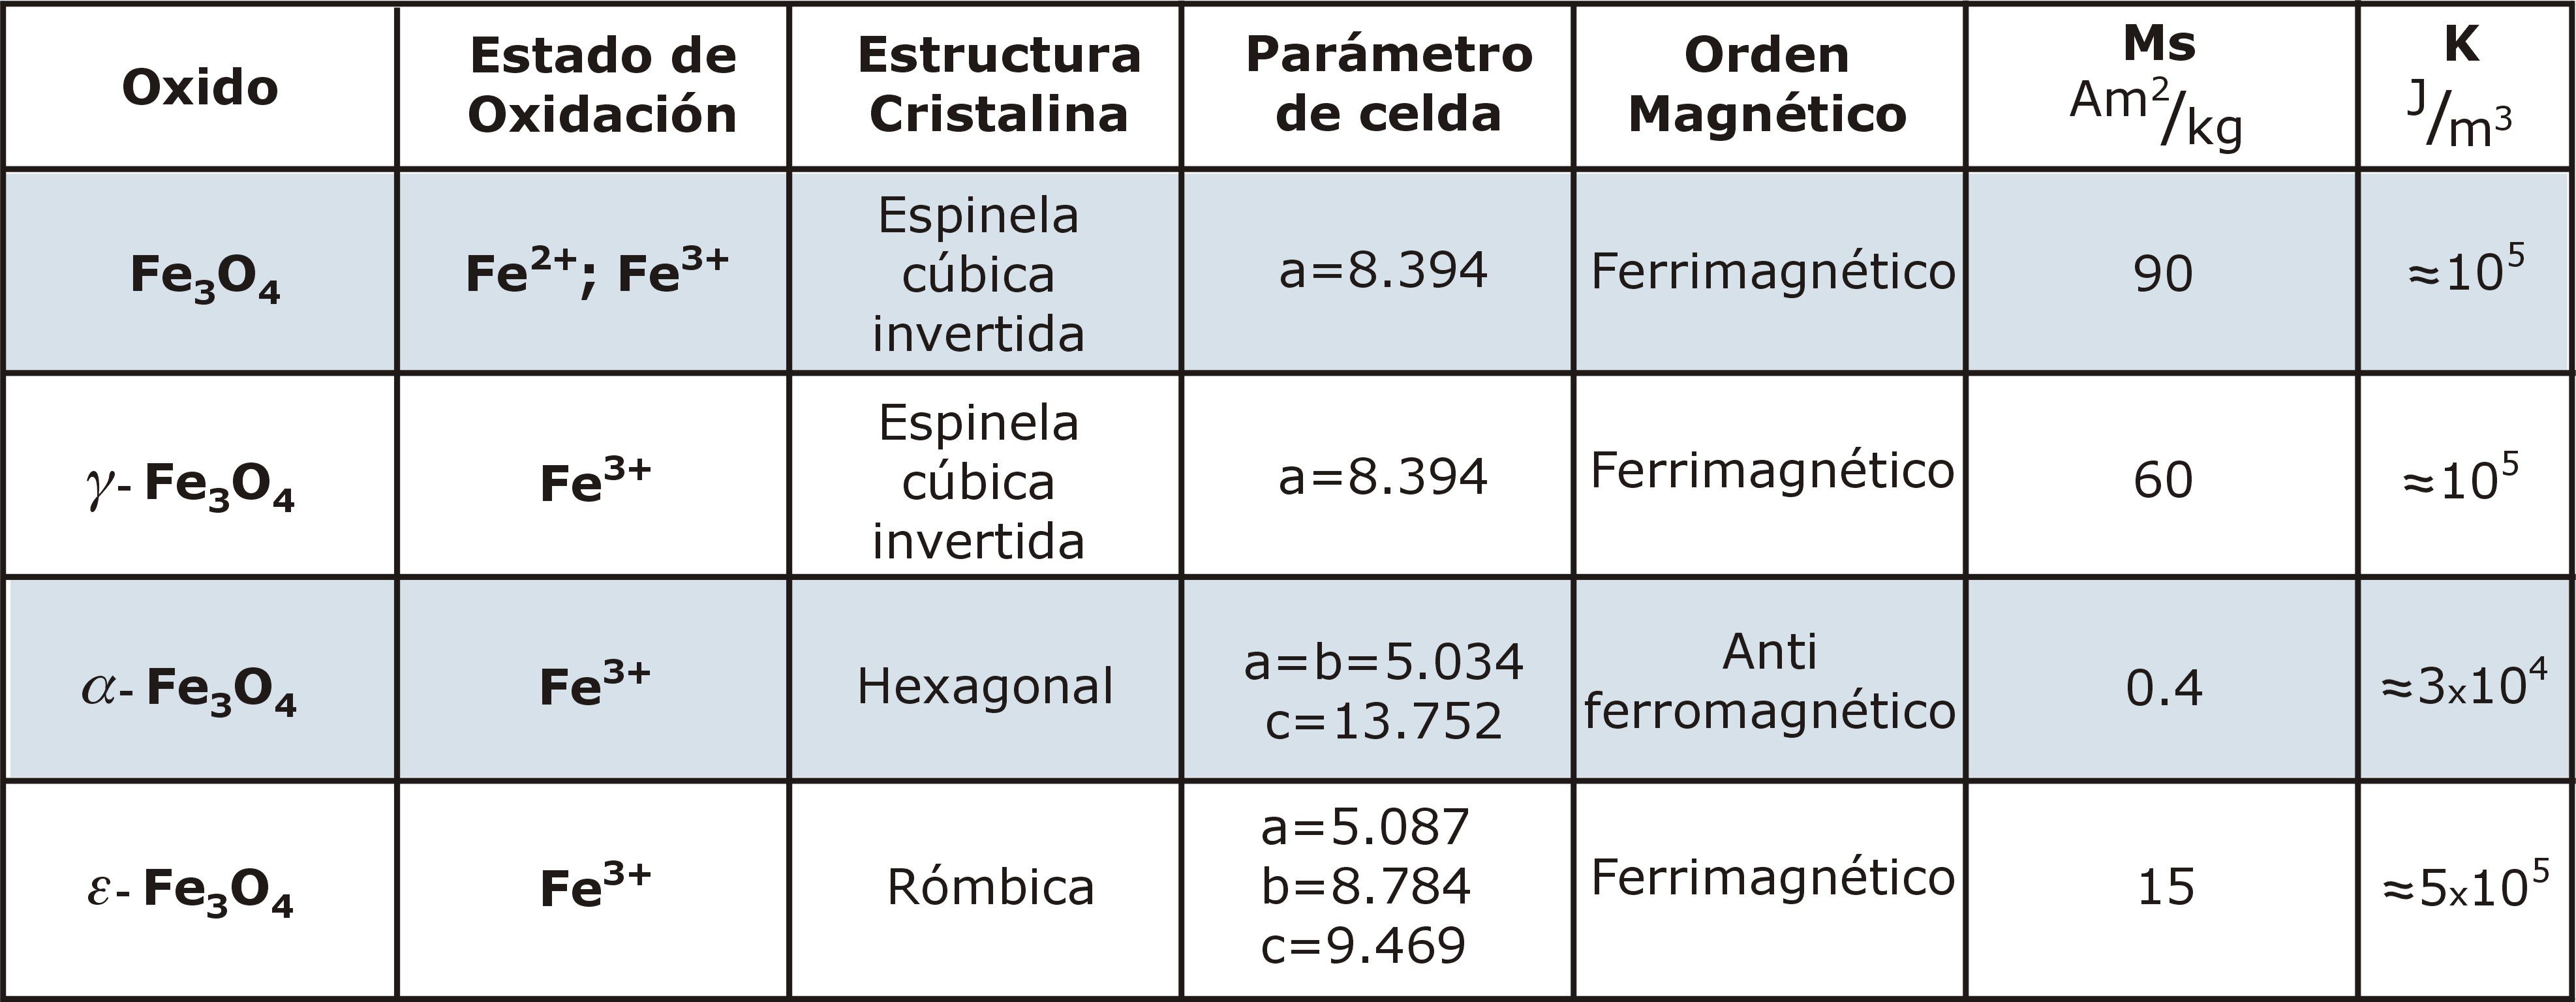
\includegraphics[width=1.0\textwidth]{./Figures/tablaDeOxidos}
	\caption{Tabla de óxidos del $Fe$}
	\label{fig:tablaDeOxidos}
\end{figure}	
	
	
	\item Las ferritas con estructura de espinela, tienen la configuración de ''espinela normal” o ''espinela inversa”.

	\item Aquellas con estructura de espinela normal son antiferromagnéticas, donde el momento magnético de los átomos que están en huecos octaédricos se anulan; entre ellas se encuentran la ferrita de cinc y cadmio ${(A^{2+})[Fe_{2}^{3+}\uparrow\downarrow]O_{4}}$.
	
\begin{figure}[H]
    \centering
    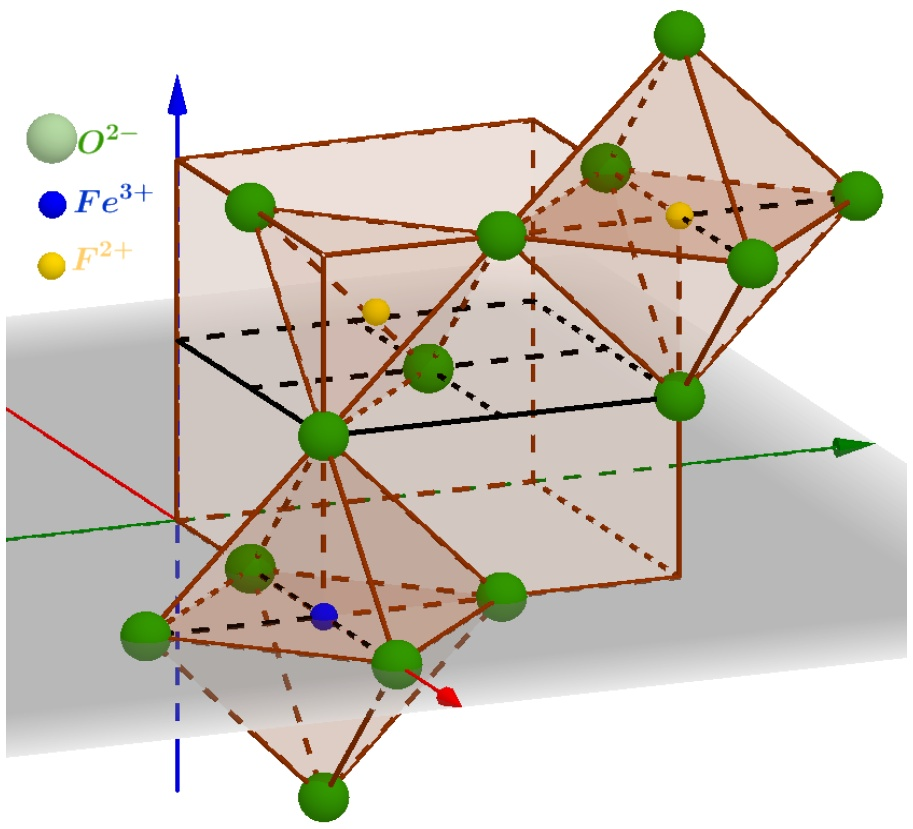
\includegraphics[width=0.6\textwidth]{./Figures/FeComplejo}
	\caption{Espinela inversa}
	\label{fig:FeComplejo}
\end{figure}

	\item Las que poseen estructura de espinela inversa son ferrimagnéticas, el momento magnético de un átomo situado en posición tetraédrico está alineado de forma antiparalela al momento magnético del sitio octaédrico. Aquí se encuentran ferritas de magnesio, manganeso, cobre, níquel, hierro, entre otros; ${(Fe^{3+}\downarrow)[A^{2+}\uparrow Fe^{3+}\uparrow]O_{4}}$.

\begin{figure}[H]
    \centering
    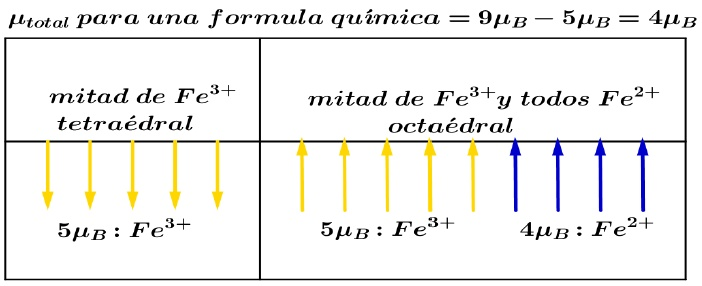
\includegraphics[width=0.6\textwidth]{./Figures/espinela2}
	\caption{$\mu_{total}$ de la Espinela inversa}
	\label{fig:espinela2}
\end{figure}

\end{itemize}

\section{Dominios magnéticos}

\begin{itemize}
	\item La importante interacción entre átomos vecinos genera una orientación espacial, estableciendo un ordenamiento llamados dominios magnéticos.
	
	\item	Un dominio magnético es una región dentro de un material magnético que tiene magnetización uniforme. Esto significa que los momentos magnéticos de los átomos individuales están alineados uno con el otro y que apuntan en la misma dirección. Esto minimiza la energía de intercambio, pero, se a creado un imán poderoso, con una energía magnetoestática muy alta. Se debe llegar a una configuración que haga mínimo ambas, por esta razón se crean los dominios. Véase la figura \ref{fig:dominioGrano1a}

	\item La dirección de alineación varía de dominio a dominio de una manera más o menos aleatoria.
	
	\item En 1906 Pierre Weiss sugirió la existencia de dominios magnéticos en materiales ferromagnéticos.
	
	\item Dentro de un monocristal las direcciones de magnetización son pocas y dependen de las propiedades de simetría de la estructura cristalina (ver figura \ref{fig:dominiosMag}). Estas propiedades definen una anisotropía, es decir, direcciones fáciles para la magnetización para las cuales la energía es mínima. Pequeñas partículas de tamaño entre $10^{-9}$ y $10^{-7}$ m presentan dominios únicos.
 
\end{itemize}


\begin{figure}[H]
	\centering
    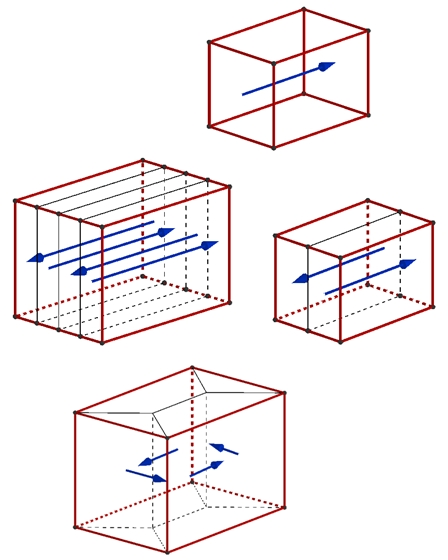
\includegraphics[width=0.60\textwidth]{./Figures/dominiosMag}
    \caption{Dominios magnéticos}
    \label{fig:dominiosMag}
\end{figure}


Una gran región de material ferromagnético con una magnetización constante, creará un gran campo
magnético que se extiende en el espacio fuera de sí mismo. Esto requiere una importante cantidad de
energía magnetostática almacenada en el campo. Para reducir esta energía, la muestra se puede dividir en dos dominios, con la magnetización en direcciones opuestas en cada dominio, reduciendo el campo fuera del material. Para reducir la energía del campo aún más, cada uno de estos dominios puede dividir también, lo que resulta dominios más pequeños con magnetización en direcciones alternas. Los ferrimagnéticos también están compuestos por dominios, cada uno de estos posee una magnetización en una cierta dirección. El cambio de la dirección de $M$ en una partícula macroscópica necesita del desplazamiento de las paredes de los dominios. Este movimiento puede lograrse con campos magnéticos externo, como veremos más adelante. A medida que disminuye el tamaño de la partícula disminuye el dimensión y número de dominios magnéticos hasta llegar a un valor crítico $rc$ por debajo del cual es energéticamente imposible crear dominios y la partícula queda con un solo dominio en el cual todos los momentos están alineados en la dirección de fácil magnetización, es decir estado de saturación magnética (se completará la idea más adelante).

\subsection{Tamaño de Dominios}

	Un dominio que es demasiado grande es inestable, y se dividirá en dominios más pequeños. Este tamaño depende del equilibrio de varias energías (energía de intercambio y de anisotropía). Cada vez que una región del solido se divide en dos dominios, crea una “pared de dominio”.
	
Los primeros resultados para ver los dominios fueron en 1931 realizados por P.A. Thiessen en Alemania y F. Bitter en USA. Ver figura \ref{fig:dominioGrano1a}


\begin{figure}[H]
	\centering
%	\raggedleft
    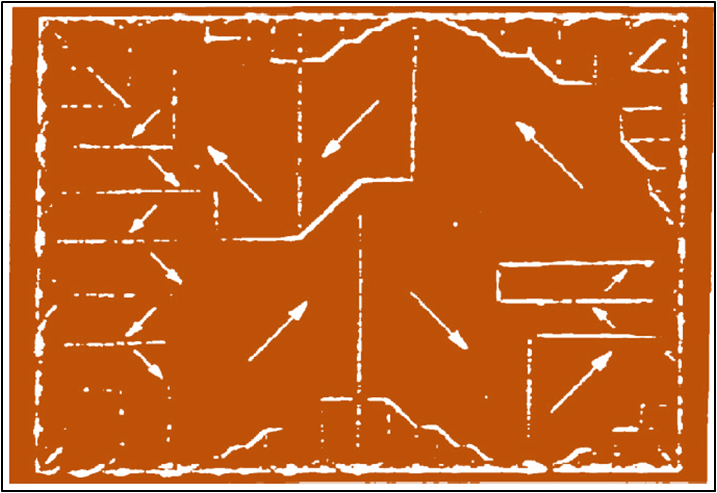
\includegraphics[width=0.60\textwidth]{./Figures/dominio_grano1}
    \caption{Dominios magnéticos}
    \label{fig:dominioGrano1a}
\end{figure}


\subsection{Estructura de grano}

\begin{figure}[H]
\begin{minipage}[b]{0.5\linewidth}
	\vspace{0pt}\raggedright
	Lo anterior describe la estructura del dominio magnético en una red cristalina perfecta, tal como se encontraría en un único cristal de hierro. Sin embargo los materiales magnéticos son policristalinos (granos) Estos granos no son los mismos que los dominios. En la mayoría de los materiales, cada grano es lo suficientemente grande como para contener varios dominios. Ver figura \ref{fig:dominioGrano2}

\vspace{1.2cm}

\end{minipage}
\begin{minipage}[b]{0.5\linewidth}
	\raggedleft
    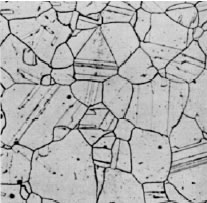
\includegraphics[width=0.90\textwidth]{./Figures/dominio_grano2}
    \caption{Bordes de grano}
    \label{fig:dominioGrano2}
\end{minipage}
\end{figure}


\subsection{Paredes de Bloch}

\begin{itemize}
	\item En el esquema se observa una representación de cómo cambian los momentos magnéticos de los átomos (M), al pasar de un dominio (A) a otro (B).
	
	\item Los dominios están separados por paredes, llamadas de Bloch, en las cuales la orientación de los momentos magnéticos atómicos cambia gradualmente de uno a otro dipolo. En el esquema el cambio de orientación es de $180^{o}$, hay también cambios de $90^{o}$ en los momentos magnéticos. Ver figura \ref{fig:dominioGrano3}

	\item Las dimensiones de los dominios son de aproximadamente $10-100 \mu m$.

	\item La dimensiones de las paredes es de aproximadamente $100nm$, unos $300$ diámetros atómicos.

	\item La magnetización dentro de los dominios magnéticos está en la dirección de los ejes cristalográficos.
\end{itemize}

\begin{figure}
	\centering
    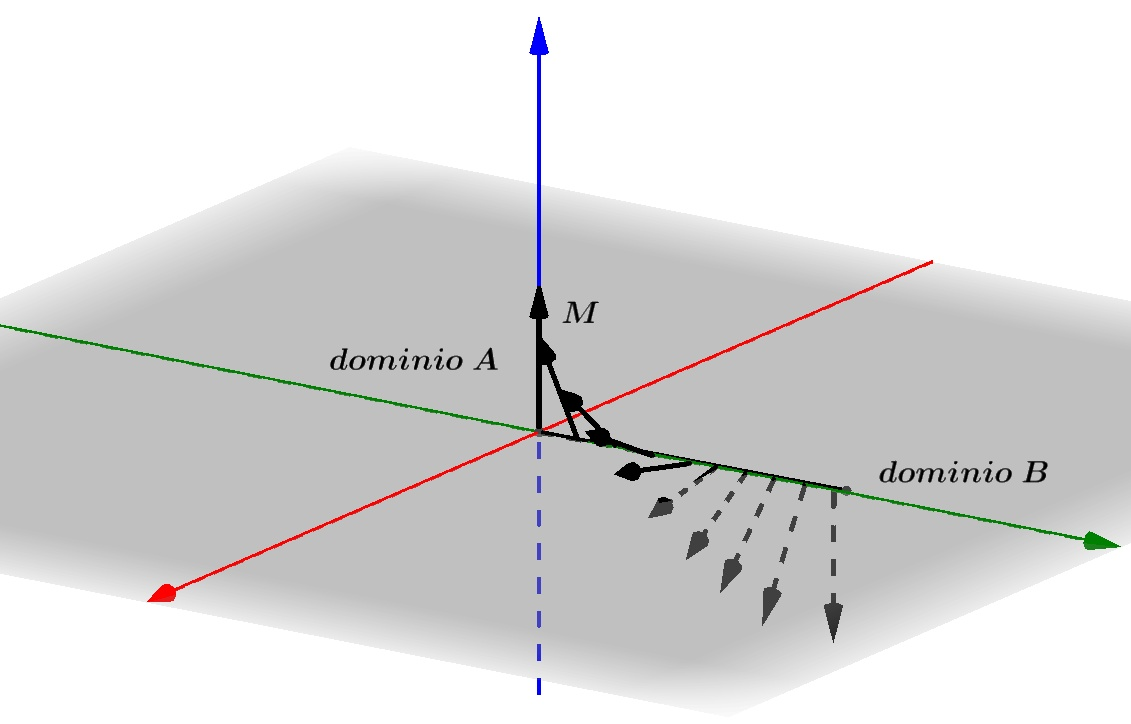
\includegraphics[width=0.95\textwidth]{./Figures/dominio_grano3}
    \caption{Transición de la pared de Bloch}
    \label{fig:dominioGrano3}    
\end{figure}

\subsection{Histéresis Magnética, movimiento de dominios}


\begin{figure}[H]

\begin{minipage}[b]{0.45\linewidth}
	\raggedright
    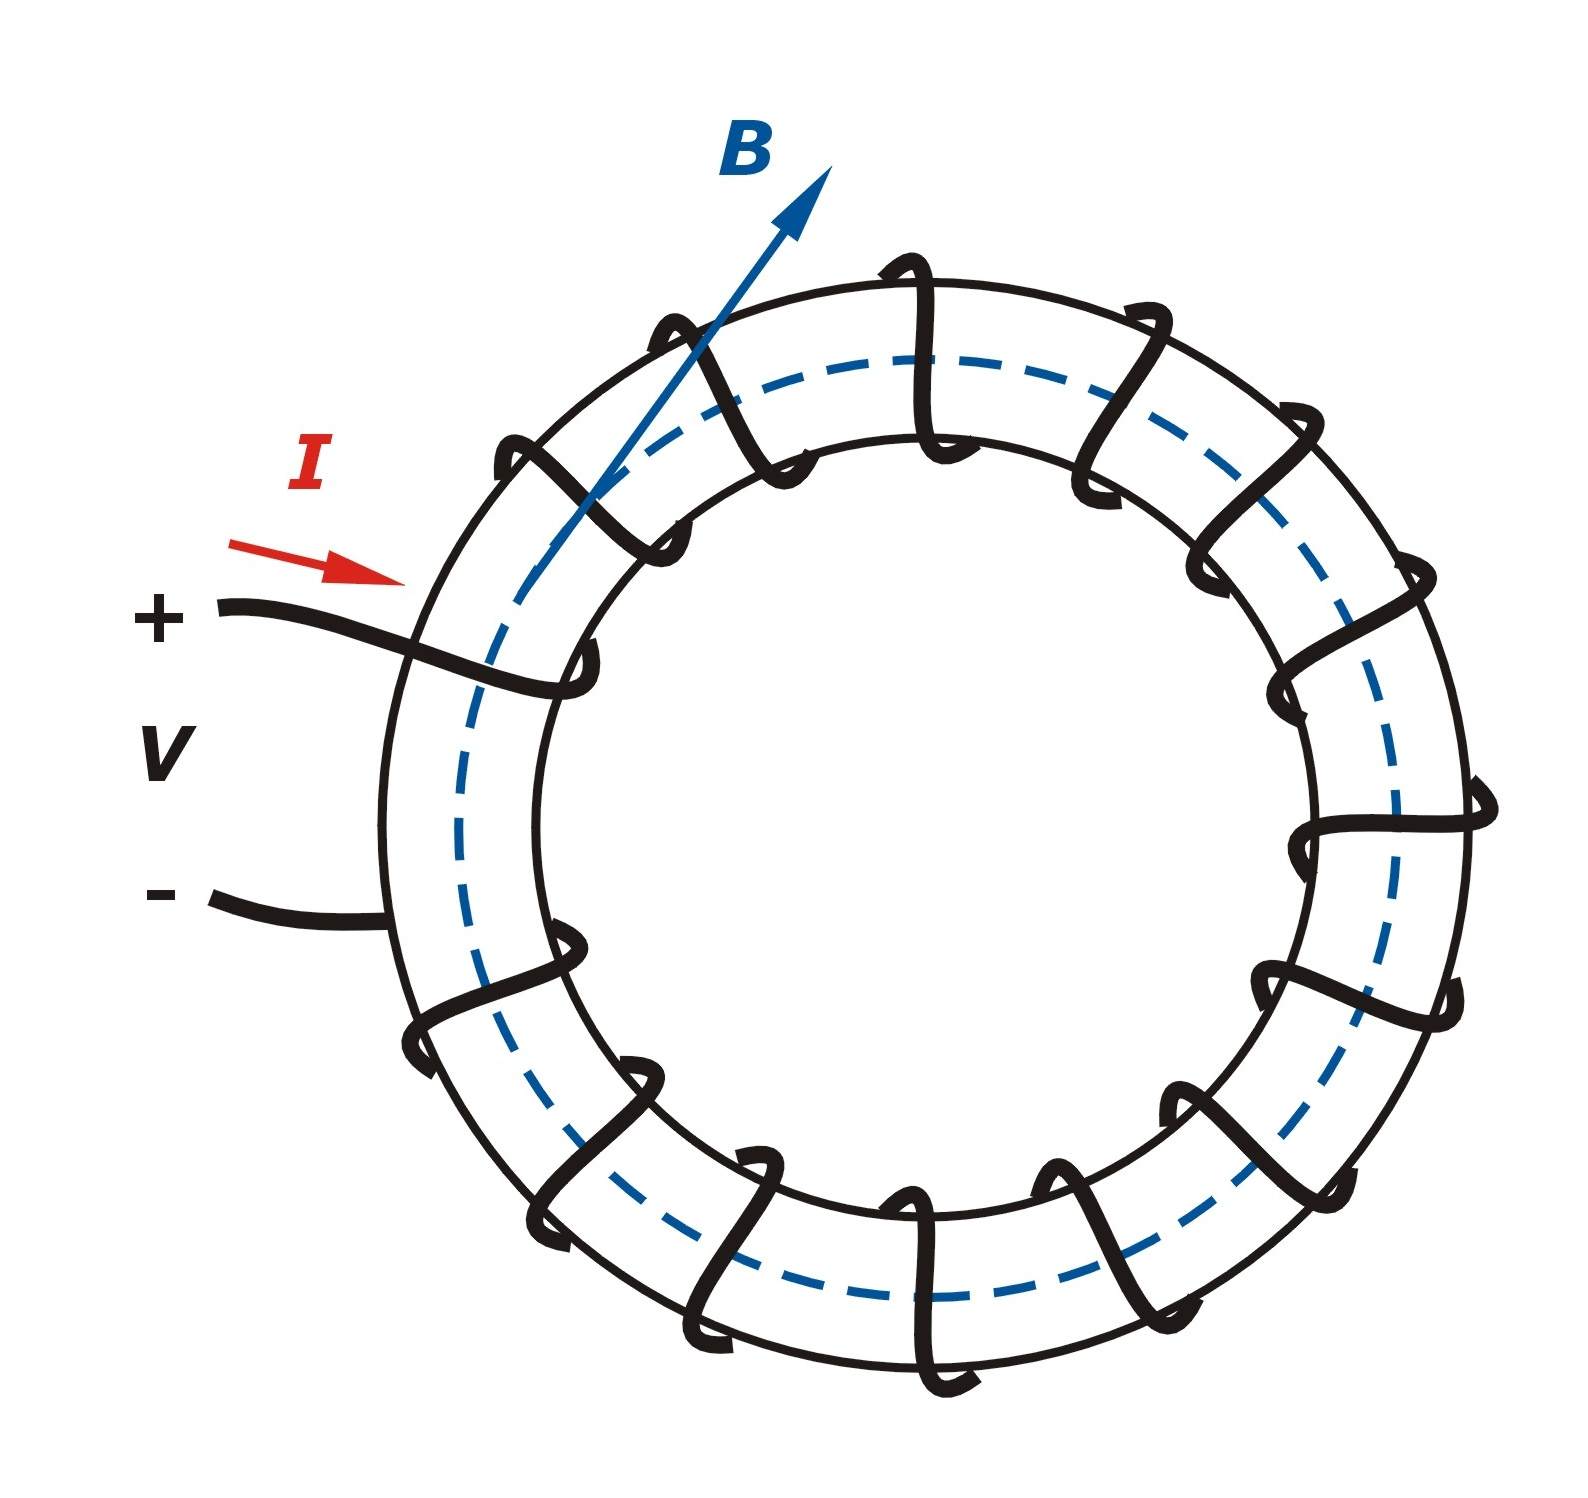
\includegraphics[width=1.0\textwidth]{./Figures/toroide}
    \caption{I y B en un toroide}
    \label{fig:toroide}
\end{minipage}
\begin{minipage}[b]{0.50\textwidth}
	\vspace{0pt}
	Como vimos los materiales ferromagnéticos y los ferrimagnéticos están constituidos por dominios y cada uno posee una magnetización espontánea en una dada dirección, pero la magnetización total sigue nula. Para cambiar las dirección de $M$ en un sólido con varios dominios se deben desplazar las pared de los dominio.\\
	
Este movimiento de los dominios se logra aplicando un campo exterior $H$. Ver figura \ref{fig:toroide}

\vspace{1.0cm}

\end{minipage}

\end{figure}

Supongamos que queremos magnetizar una barra toroidal como la de la figura \ref{fig:toroide}, a una dada temperatura de un material ferromagnético originalmente desmagnetizado. Para tal fin medimos $M$ en función del campo magnético aplicado $H$, siendo el campo magnético función de la corriente eléctrica $I$. Graficando $M$ en función de $H$ obtendremos una curva como la de la figura \ref{fig:primeraImanacion}

\begin{figure}[H]
    \centering
    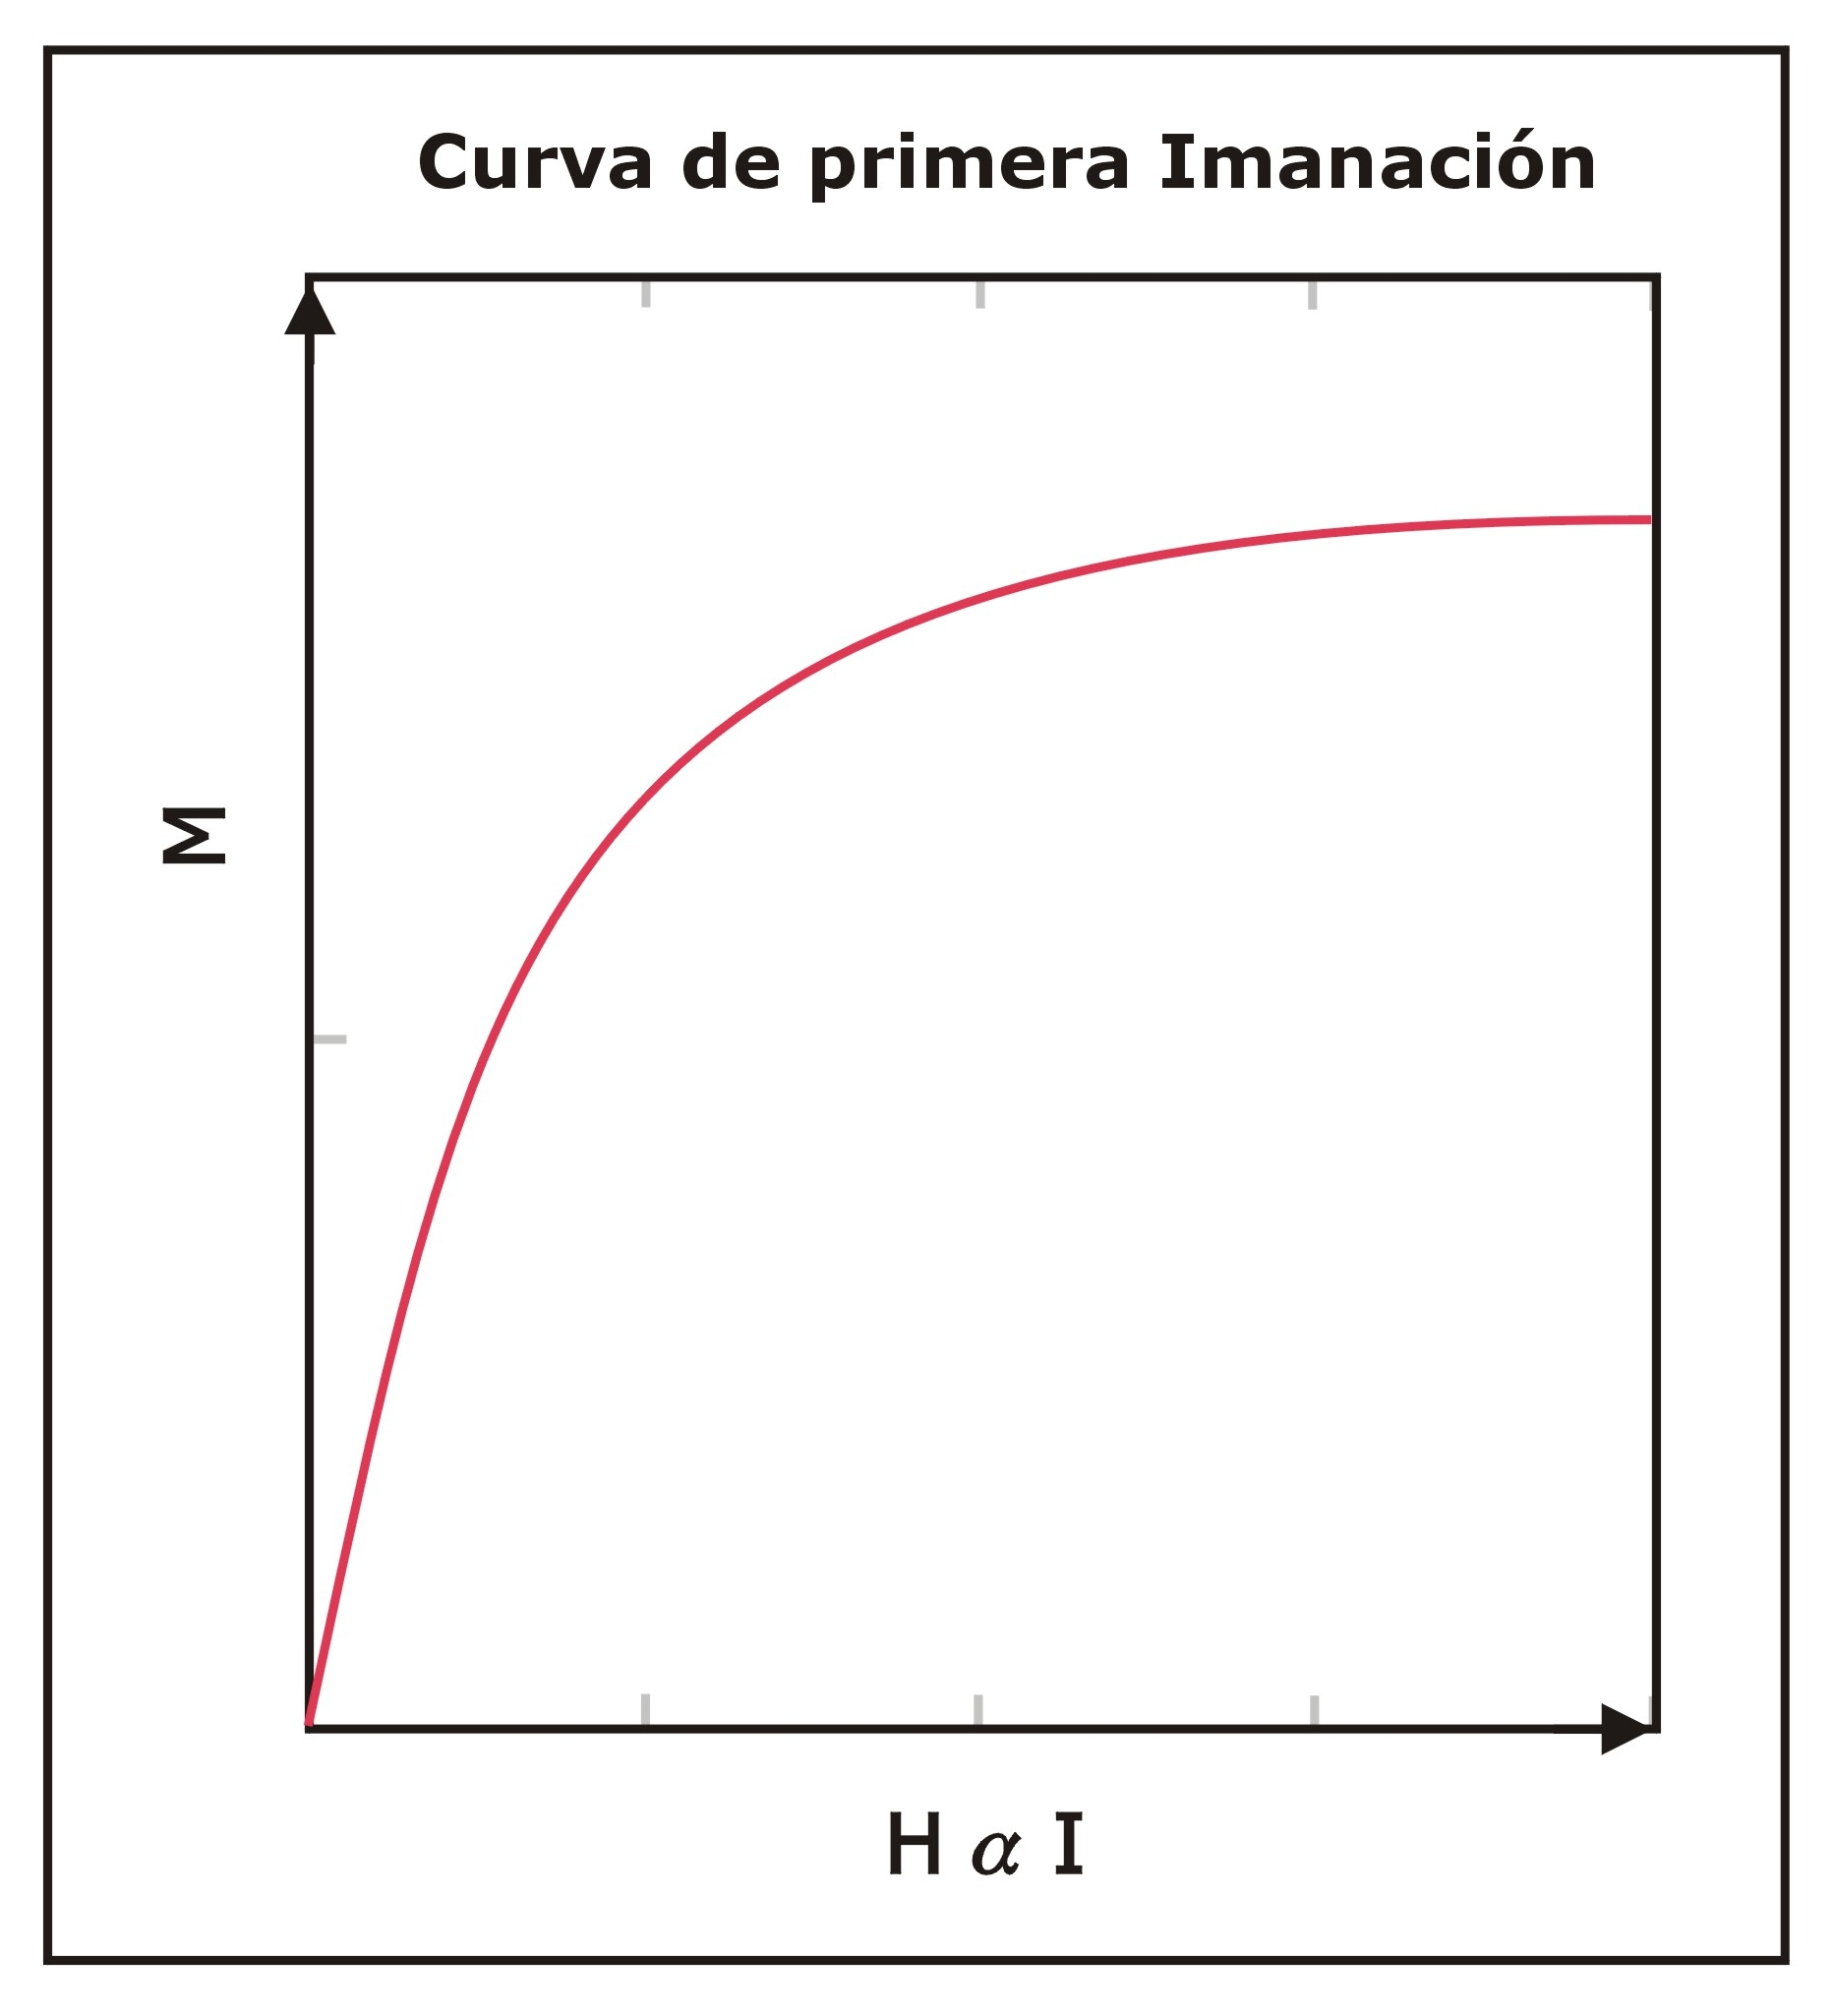
\includegraphics[width=0.6\textwidth]{./Figures/primeraImanacion}
	\caption{Curva de primera imanación}
	\label{fig:primeraImanacion}
\end{figure}


\section{Ciclo de Histéresis}

La magnetización de saturación $M_{s}$ es el valor máximo que puede alcanzar la magnetización en el material, por mas que continuemos aumentando $M$.

Cuando disminuimos el campo $H$ y llegamos a cero la magnetización no es cero por el contrario permanece una magnetización $M_{R}$, magnetismo remanente. Para poder llevar la magnetización a cero debemos invertir el sentido del campo hasta $-H_{c}$, llamado \textbf{Campo coercitivo}.

Durante el crecimiento del campo $H$ los dominios magnéticos favorecidos por el campo crecen a costa de los más desfavorables. Solo rotan en la última etapa próxima a la saturación. 

El giro completo de los momentos magnéticos atómicos de un dominio al vecino no es realizado en un
único plano, sino que debe ser realizado a través de varias distancias atómicas. Como fue esquematizado en la pared de Bloch. 

Si de alguna manera logramos que muchos dominios tengan permanentemente una componente de magnetización en una dirección común, estaremos en presencia de un imán permanente.

\subsection{Pérdidas por Histéresis}

En los materiales magnéticos sometidos a la acción de campos variables,(corrientes alternas) hay fundamentalmente dos tipos de pérdida de energía, una de ellas es por histéresis, que veremos ahora, y la otra es por \textbf{corrientes parásitas}.

Sabemos que la $fem$ inducida en un solenoide es

\begin{equation}
\varepsilon = - N\,S\, \frac{dB}{dt}\quad \text{donde $N$ es el número de espiras y $S$ el área} 
\end{equation}

luego la potencia será

\begin{equation}
P = \varepsilon\,i = - N\,S\,i\, \frac{dB}{dt}\quad 
\end{equation}


también sabemos que $i=\frac{HL}{N}$, siendo $L$ la longitud del solenoide (ver figura \ref{fig:toroide}) 

\begin{equation}
\begin{aligned}
P = S\; L \; H \frac{dB}{dt} \; = \; V \; H \frac{dB}{dt} \; = \; \frac{dW}{dt} \\
dW = V H dB \Rightarrow W = V \oint H dB 
\end{aligned}
\end{equation}

Si integramos en un ciclo y por unidad de volumen las perdidas están dadas por el área del ciclo de histéresis. Esta pérdida de energía por unidad de volumen de material, puede ser expresada por una fórmula aproximada llamada fórmula de Steinmetz.

\begin{equation}
P_{h} = K f B_{max}^{\alpha}\left[ \frac{erg}{seg cm^{3}} \right] 
\end{equation}

Donde $K$ y $\alpha$ son parámetros característicos del material mientras que $f$ es la frecuencia y $B_{max}$ la inducción máxima. 

Donde $K$ y $\alpha$ son parámetros característicos del material mientras que $f$ es la frecuencia y $B_{max}$ la inducción máxima. El valor de $K$ para el hierro dulce es $\cong 54x10^{−5}$, para el acero $\cong 337x10^{−4}$.

Generalmente $\alpha = 1,6$. Para mediciones más precisas, especialmente a inducciones relativamente bajas ${\alpha\rightarrow 2}$. Estas pérdidas generan un aumento de temperatura del sistema.


\subsection{Pérdidas por Corrientes parásitas}

Si el campo magnético $H$ es alterno produce otro tipo de pérdida que debemos sumar a las pérdidas por histéresis. Según la Ley de Lenz se genera una $fem$ y si el material es conductor se crean corrientes eléctricas (corrientes turbillonarias o de Foucault) ocasionando pérdidas de energía a través del efecto Joule también llamadas corrientes parásitas o de Eddy. Ver figura \ref{fig:corrientesParasitas2}

\begin{figure}[H]
    \centering
    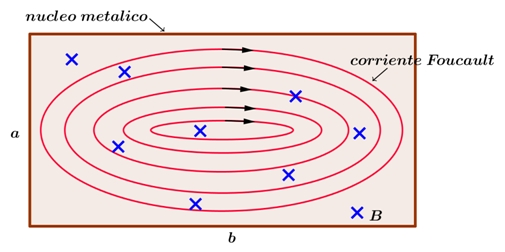
\includegraphics[width=0.8\textwidth]{./Figures/corrientesParasitas2}
	\caption{Flujo de corrientes Eddy }
	\label{fig:corrientesParasitas2}
\end{figure}

Analicemos la figura \ref{fig:corrientesParasitas1} y supongamos que el campo magnético es ${B = B_{0} Sin(\omega t)}$. Calculemos la resistencia eléctrica de una espira ideal de la chapa suponiendo que $\alpha\ll b$ siendo el espesor $dx$ a una distancia $x$ y largo $c$

\begin{equation}
R = \rho \frac{l}{S} = \rho \frac{2 b}{c dx}
\end{equation}

\begin{figure}[H]
    \centering
    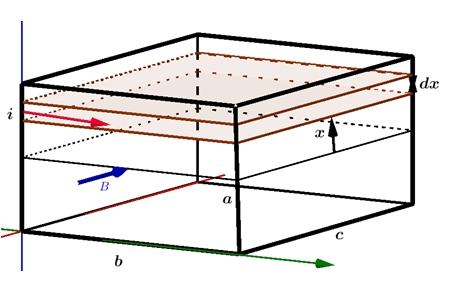
\includegraphics[width=0.6\textwidth]{./Figures/corrientesParasitas1}
	\caption{Elemento de Resistencia}
	\label{fig:corrientesParasitas1}
\end{figure}

Y el flujo será:
$\Phi = B(t)S = 2 b x B_{0} sin(\omega t)$

Mientras que la $fem$ inducida será:
$e = \frac{d\Phi}{dt} = 2 b x B_{0} Cos(\omega t)$

Luego, la corriente será:

\begin{equation}
\begin{aligned}
i= \frac{e}{R} = \frac{2 b x B_{0} Cos(\omega t) dx}{2bp} = \frac{c \omega x B_{0} Cos(\omega t)}{\rho}
\end{aligned}
\end{equation}

Calculemos la potencia media en un período $T$ y en toda la chapa:

%\begin{equation}
\begin{multline}
\overline{P}= \frac{1}{T}\int_{0}^{T}dt\int_{0}^{\mfrac{a}{2}} \frac{2 b c B_{0}^{2}\omega^{2}Cos^{2}(\omega t)}{\rho}dx
 =  \frac{2 b c B_{0}^{2}\omega}{\rho T} \int_{0}^{T} Cos^{2}(\omega t) d(\omega t) \int_{0}^{\mfrac{a}{2}}x^{2} dx = \\
\frac{2 b c B_{0}^{2}\omega}{\rho T} \left[ \left( \frac{a}{2}\right)^{3} \right] \left[ \frac{\omega T}{2} \right] = \frac{b c a^{3} B_{0}^{2} \omega^{2}}{24 \rho} = \frac{a^{2} B_{0}^{2} \omega^{2}}{24 \delta \rho} 
\end{multline}
%\end{equation}

En la última expresión se paso a densidad $(\delta)$ , luego las unidades de potencia estarán dada en $\left[ \frac{Watt}{Kg}\right] $

Observemos que: las pérdidas por corrientes parásitas son proporcionales al cuadrado de la inducción máxima y de la frecuencia, ambas dos dependen de la excitación. Del material dependen la resistividad y la densidad, vemos que cuando más elevada es la resistividad menor serán las perdidas. Hay una magnitud de carácter geométrico $\alpha$, en la expresión anterior, que se encuentra elevada al cuadrado, es el espesor de la chapa. Cuanto menor sea el espesor de la chapa tanto más pequeñas serán las pérdidas.

\subsection{Comentarios sobre las corrientes de Foucault}

Esta es la razón por la cual los equipos eléctricos que funcionan con corriente alterna están constituidos por chapas muy delgadas, aisladas entre sí, para disminuir lo más posible estas pérdidas. Vimos que estas corrientes dependen de la resistividad del núcleo, o bien, podemos usar un material ferromagnético elevada resistividad caso de la ferrita o bien agregando un aliante: $Si$ al hierro que eleve la resistividad sin modificar apreciablemente las propiedades magnéticas. 

Al no poder los electrones atravesar la capa aislante entre las chapas, se acumulan en los extremos de la laminado como se observa en la figura \ref{fig:Foucault} en forma similar al efecto Hall, la fuerza responsables es:


\begin{equation}
\vec{f_{m}} = e\, \vec{v} \times \vec{B}
\end{equation}

\begin{figure}[H]
    \centering
    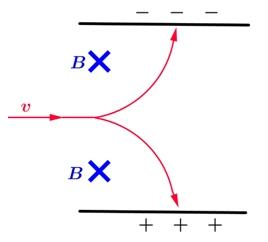
\includegraphics[width=0.5\textwidth]{./Figures/Foucault}
	\caption{Cargas en los extremos del laminado}
	\label{fig:Foucault}
\end{figure}

la acumulación de cargas produce un campos eléctricos $\vec{E_{m}}$ que se oponen a una mayor acumulación de cargas, la fuerza generada por este campo eléctrico es:

\begin{equation}
\vec{f_{m}} = e\, \vec{E_{m}}
\end{equation}

si son iguales ambas fuerzas tendremos:

\begin{equation}
e\, \vec{E_{m}} = e\, \vec{v} \times \vec{B} \rightarrow \vec{E_{m}} = e\, \vec{v} \times \vec{B}
\end{equation}

de donde podemos calcular la diferencia de potencial. ¿Qué magnitud tendrá, esta diferencia de potencial en un trasformador común? y ¿en qué la podríamos utilizar?.

Las corrientes de Foucault son también la causa del efecto pelicular en conductores de corrientes alternas.


\subsection{Materiales magnéticos duros y blandos}

El fundamento de la clasificación de los materiales magnéticos en blando(dulces) y duros se debe a las distintas aplicaciones de uno y otro Un material magnético blando es fácilmente magnetizable y desmagnetizable, mientras que uno duro tiene propiedades totalmente distintas. Como sabemos estas propiedades están íntimamente ligadas al ciclo de histéresis de cada material. Un acero blando de hierro silicio 3−4\% $Si$ es utilizado en núcleos de transformadores, motores, generadores y tiene un ciclo de histéresis con baja fuerza coercitiva y un área pequeña, mientras que un material magnético duro posee un amplio ciclo de histéresis con una importante fuerza coercitiva Su uso es frecuente en imanes permanentes

\textbf{Hierro silicio (fines 1800)}. La utilización de aleaciones de hierro silicio 3−4\% $Si$ trae aparejado los siguientes beneficios en las maquinas eléctricas.

$\ast$ El agregado de silicio al hierro de bajo carbono, disminuye las perdidas por corriente parasitas.

$\ast$ Aumenta la permeabilidad magnética y disminuye la anisotropía magnética bajando las perdidas por histéresis.

$\ast$ También disminuye la magnetostricción bajando el clásico zumbido 

El efecto negativo del agregado de silicio es que disminuye la ductilidad de la ferrita y disminuye la temperatura de Curie. Es posible mejorar la
característica del hierro silicio logrando la aleación con grano orientado. La presencia del C en el Fe lo endurece mecánica y magnéticamente, ya que
genera cementita, $Fe3C$, que impide el movimiento de paredes de dominios.

\textbf{Permalloy (1914)}. Es el nombre comercial de una aleación de aproximadamente 80\% $Ni$ y 20\%$Fe$. Existen otras aleaciones, por ejemplo el permaloy 45 que contiene 45\%$Ni$ y 55\%$Fe$, o bien el permalloy molibdeno es una aleación con el 81\%$Ni$, 17\%$Fe$ y 2\%$Mo$. Su uso es en transformadores, reactancias, etc.

\textbf{Mumetal 1923}. Es una aleación de aproximadamente 75\%$Ni$, 15\%$Fe$ y 10\% $Cu$ o $Mo$, tiene una permeabilidad muy alta, por lo cual es usada como pantalla para brindar campos magnéticos estáticos o de baja frecuencia. Su primera aplicación fue en los cables telegráficos submarinos

\textbf{Superpermalloy o supermalloy (inicios década 40)}. Es una aleación de 75\%$Ni$, 5\%$Mo$ y 20\%$Fe$, con permeabilidad magnética alta y baja
coercitividad. Algunas de sus propiedades son comparables con el Mumetal. Esta aleación requiere tratamientos térmicos a temperatura de 1300 ${^{o}C}$ en atmosfera de hidrogeno.

\textbf{Vidrio metálico (1960 no magnético)}. Estos materiales son metales pero no tienen una estructura cristalina determinada, son amorfos. Se destacan por sus propiedades mecánicas al no poseer dislocaciones son hasta tres veces más duros que los aceros La ausencia de bordes de grano, conduce a una mayor resistencia al desgaste y a la corrosión. Son realmente vidrios auténticos, al calentarse se ablandan y fluyen. La primera aleación magnética fue llamada Metglas 2605 (década de 1980 con 80\%$Fe$ y 20\%$Bo$ con una temperatura de Curie de 373${^{o}C}$ y una magnetización de saturación de 1,56 Tesla. Sus propiedades magnéticas, como materiales magnéticamente blandos, son de baja coercitividad, elevada permeabilidad o alta magnetización de saturación. Esto permite aplicaciones en núcleos de transformadores eléctricos. También son utilizados como biomateriales para implantes óseos o recubrimientos dentales, pues, no se oxidan fácilmente. Están confeccionados en base a un material ferromagnético (hierro, cobalto o níquel), aleados con boro silicio, fosforo, entre otros.


Como hemos dicho, por la forma del ciclo de histéresis es posible clasificar a los materiales magnéticos, en principio en dos grandes grupos: magnéticamente blandos y magnéticamente duros.

Los que tienen bajo valor de coercitividad $H_{c}<800 A/m$ son los blandos y en aquellos donde la coercitividad es $H_{c} > 5000 A/m$ son los duros. Los blandos son utilizados en núcleos de maquinas eléctricas y transformadores. 

En los materiales blandos se desea ciclos de histéresis muy estrechos y altos. Los materiales duros son usados como imanes permanentes. Las propiedades más importantes de los material magnéticamente duro son su elevado campo coercitivo y su importante inducción de saturación También por la forma del ciclo de histéresis es posible caracterizar metalúrgicamente al material, como veremos más adelante.

\begin{figure}[H]
  \centering
  \begin{minipage}[b]{0.47\textwidth}
    \centering
    \vspace{0pt}
     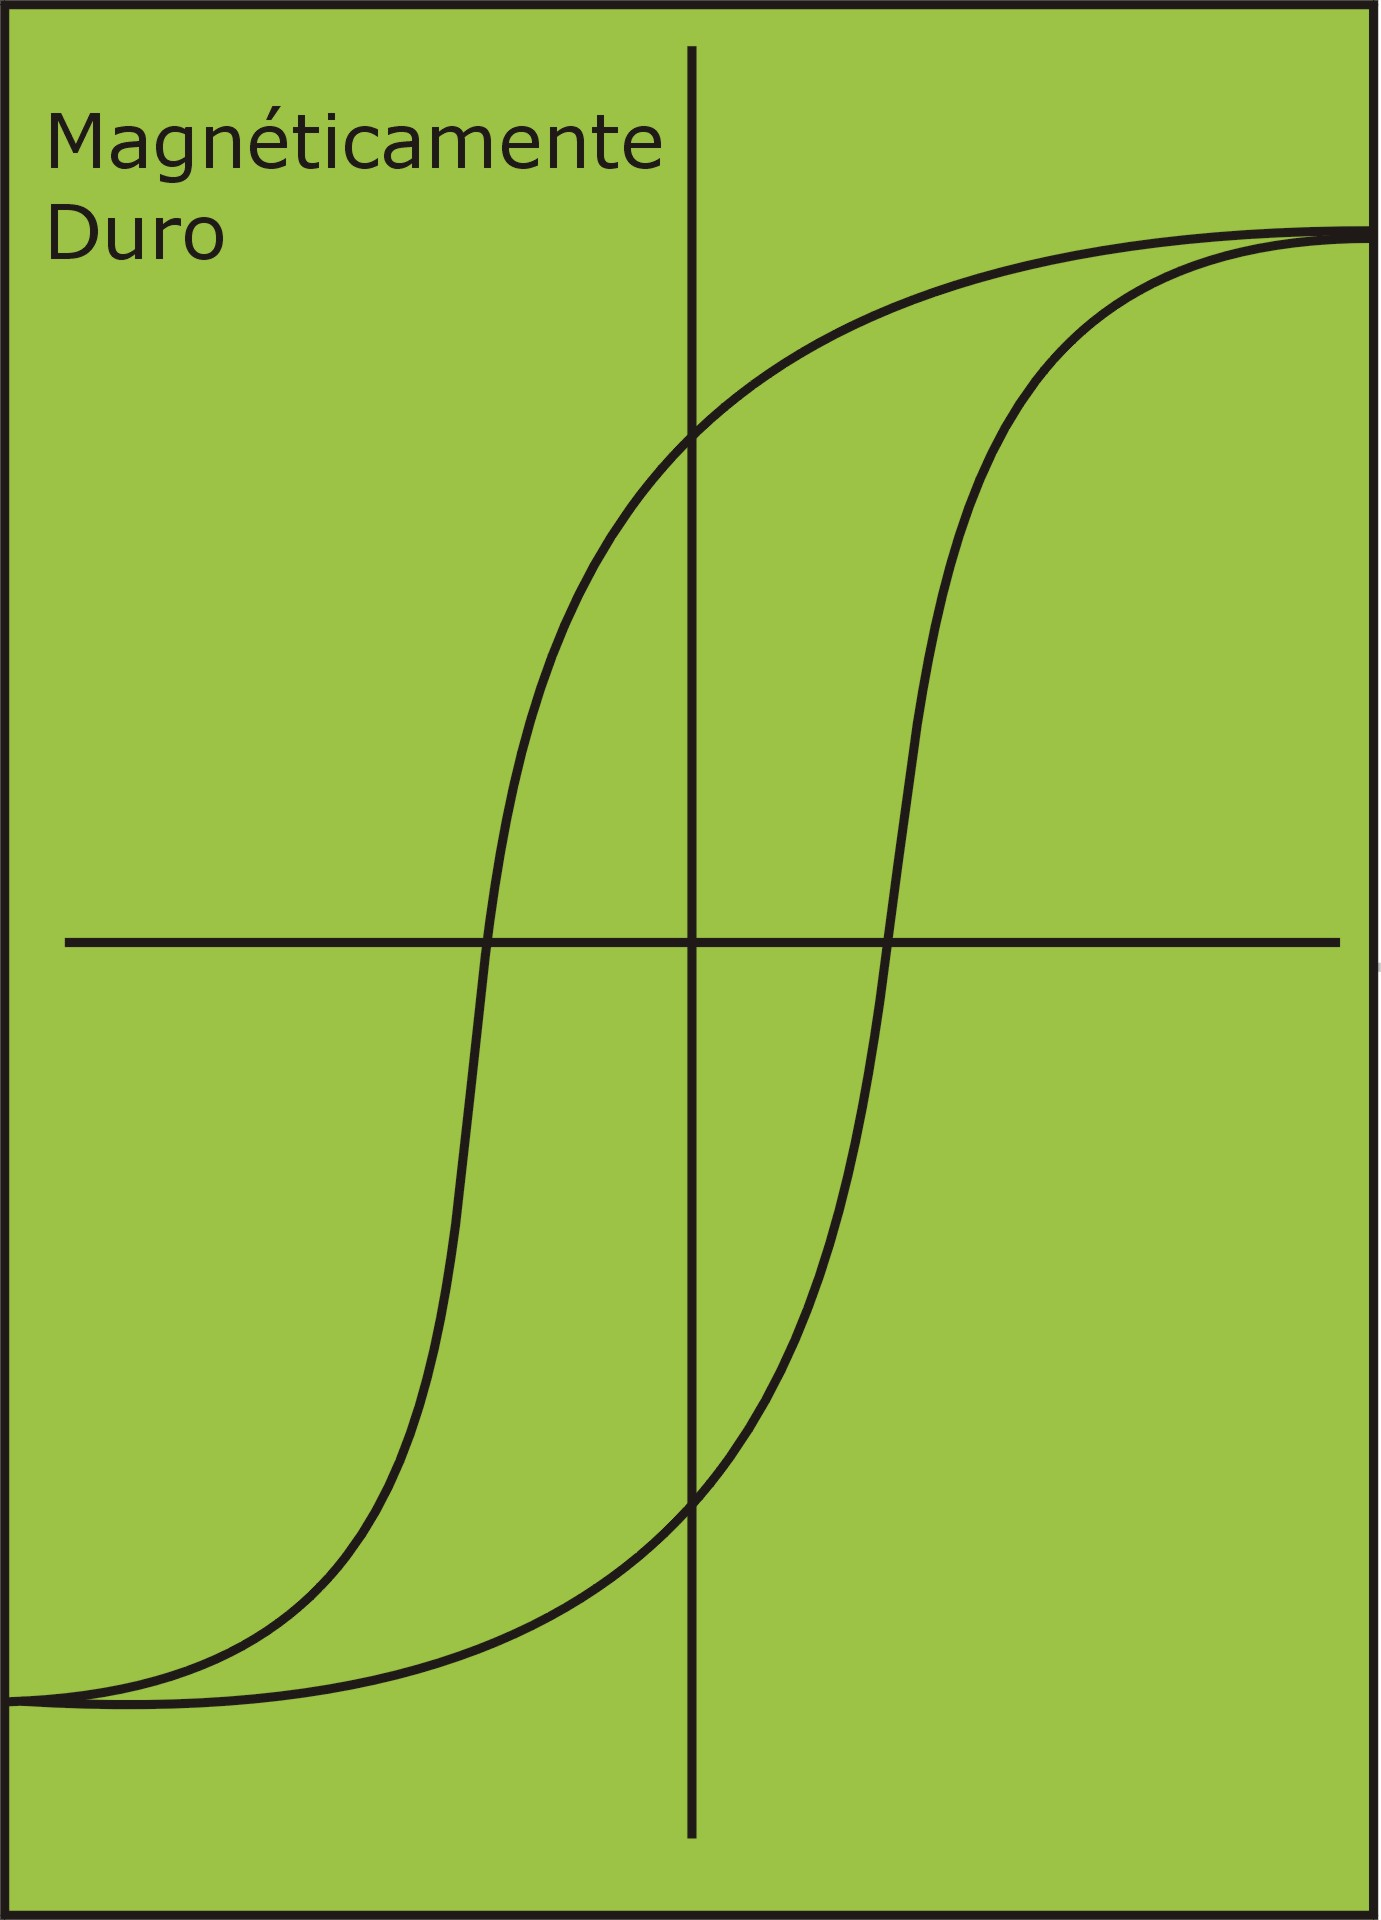
\includegraphics[width=0.9\textwidth]{./Figures/materialesDuros}
  \end{minipage}
  \hfill
  \begin{minipage}[b]{0.47\textwidth}
    \centering
    \vspace{0pt}
     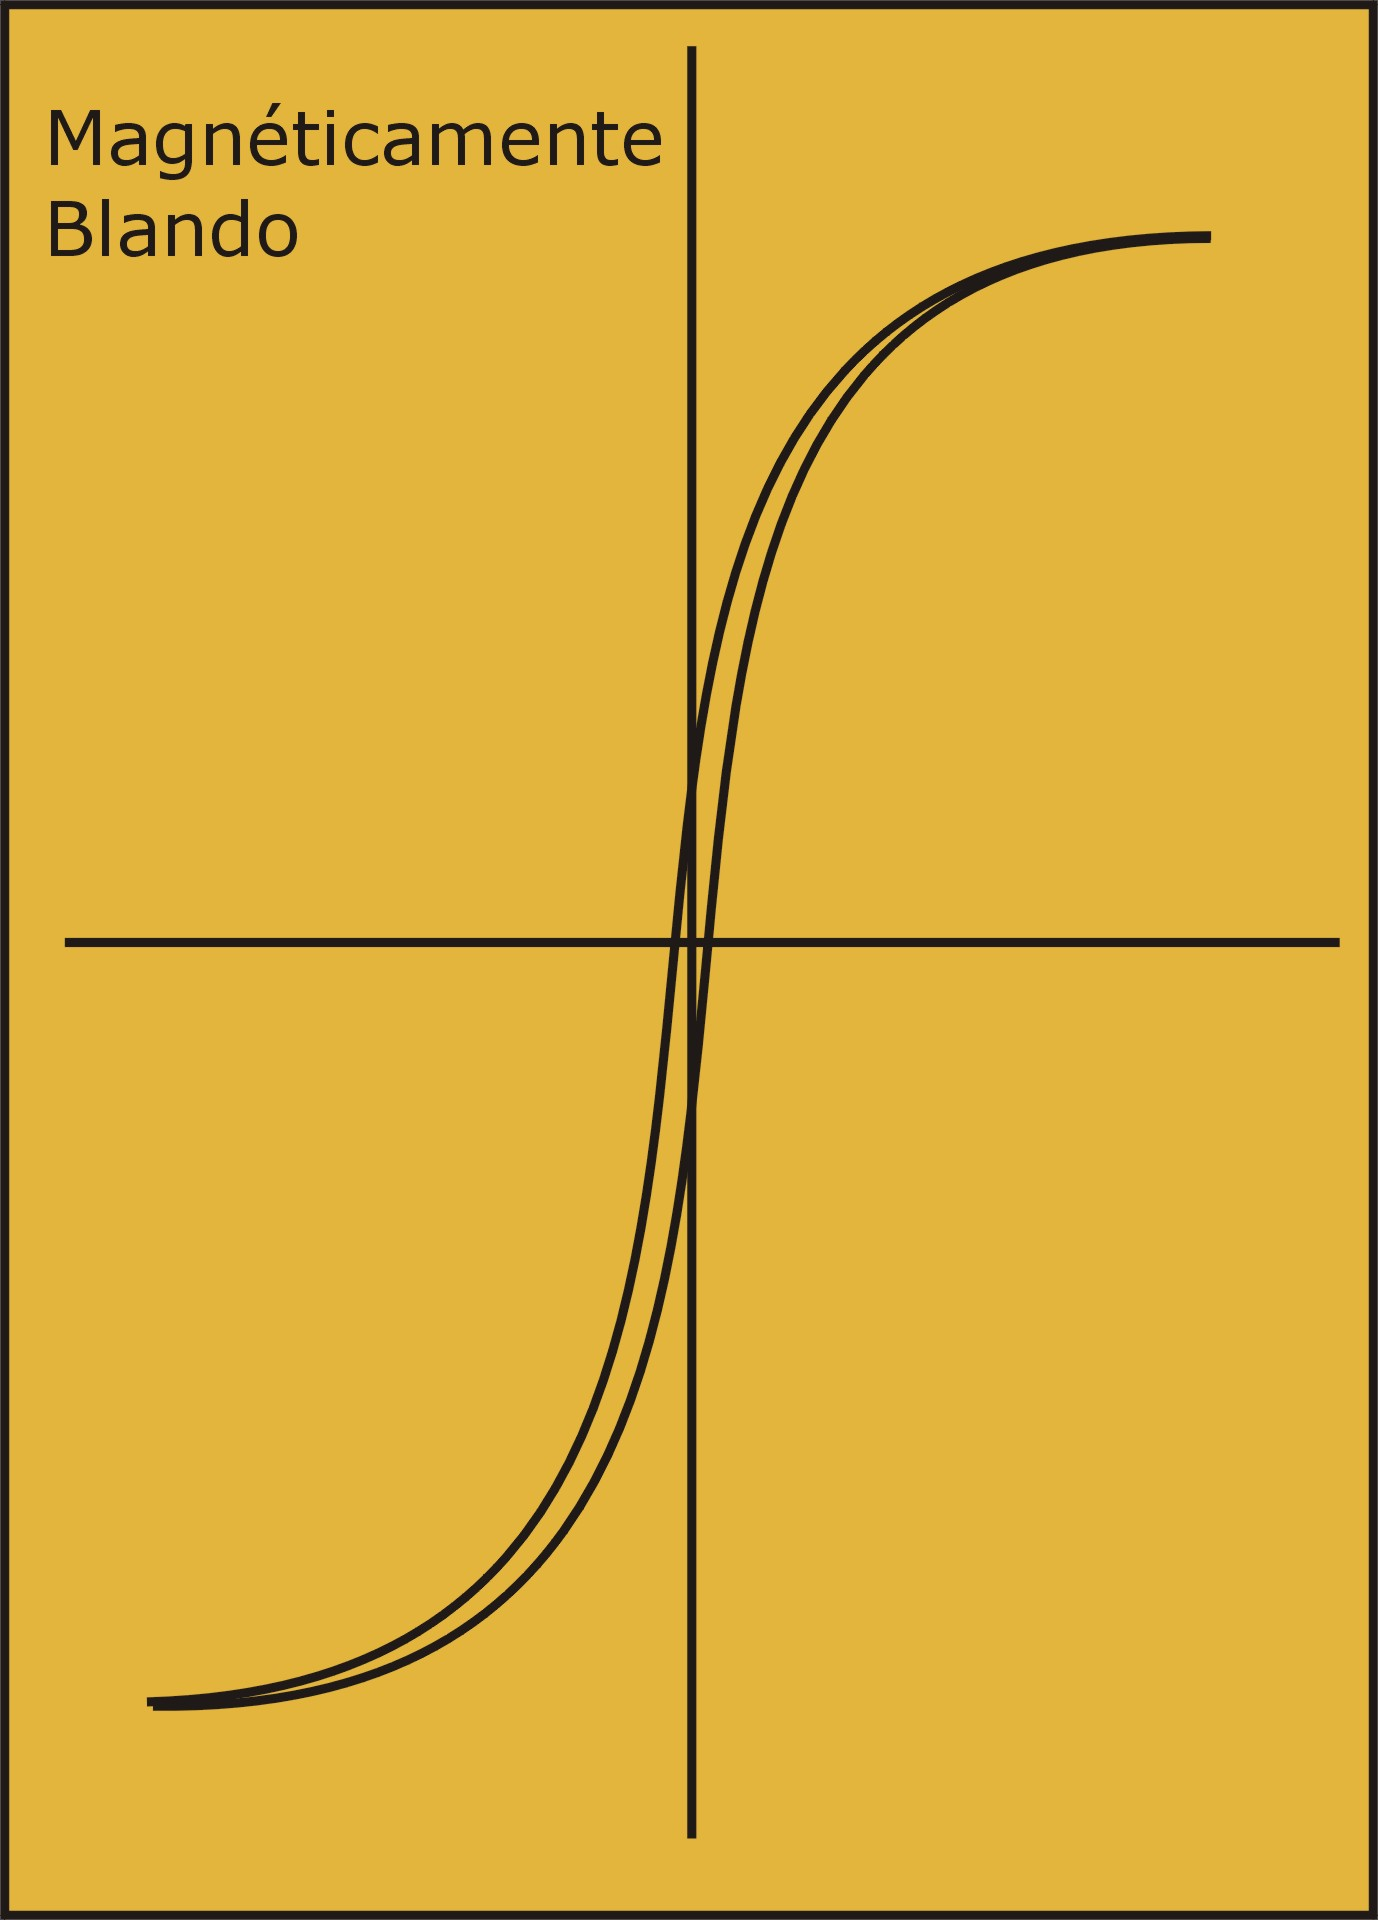
\includegraphics[width=0.9\textwidth]{./Figures/materialesBlandos}
  \end{minipage}
  
  	\label{fig:materialesDurosBlandos}

  \caption{Materiales duros y blandos}
  
\end{figure}


\subsection{Imanes permanentes}

Haremos un breve resumen de los principales materiales para los imanes permanentes.

Estos materiales deben poseer la particularidad de mantener el campo
magnético luego de ser magnetizado. El desarrollo de estos materiales se da por la necesidad de obtener importantes cantidades de energía magnética almacenada en pequeños volúmenes.

\textbf{Alnico(1931)}. Es una aleación formada principalmente por Al Ni Co de donde deriva su nombre, generalmente tienen la siguiente composición 8−12\%$Al$, 15−26\%$Ni$, 5,24\%$Co$, $\approx 6 \% Cu$, $\approx 1 \% Ti$,  resto $Fe$. Se lo fabrica por sinterizado o fundición y requiere un tratamiento térmico posterior. La temperatura de Curie es la mas alta hasta el momento $\approx$800 ${^{o}C}$, puede estar al rojo y sigue siendo magnético. Los imanes de Alnico son conductores eléctricos, a diferencia de los imanes cerámicos. Hay una gran variedad de estas aleaciones, con distintos nombres comerciales generalmente tienen una alta coercitividad, solo los imanes de tierras raras tienen mayor coercitividad. Algunas de la aleación son isótropas y pueden ser magnetizados en cualquier dirección Otros, tales como Alnico 5 y Alnico 8 son anisotrópicas, y tiene una dirección preferente de magnetización. Las Aleaciones anisotrópicas generalmente tienen mejores propiedades magnéticas en la dirección elegida 

\textbf{Imanes de tierras raras (lantánidos)}:

Recordemos que algunos cristales no presentan las mismas propiedades magnéticas según las distintas direcciones en que se las mida, o sea son
anisótropos magnéticamente hablando La anisotropía magnética es fundamental para construir imanes permanentes. En \textbf{1966} se descubre que una aleación de itrio cobalto $YCo_{5}$ tenia una constante de anisotropía 

magnética mucho mayor que los materiales conocidos a la fecha, dicho de otro modo son fácil de magnetizar en una dirección pero muy difícil en las otras. Los lantánidos son generalmente ferromagnéticos, pero con un serio inconveniente para su uso industrial, tienen una temperatura de Curie que esta por debajo de la ambiente. Este inconveniente puede ser solucionado formando compuestos con elementos de transición, como ser el hierro, níquel, cobalto, etc; logrando de este modo temperaturas de Curie mayor que la ambiente. 

Unos años después(se desarrollan los primeros imanes permanentes de tierras raras Hasta el momento los mas conocidos son dos los de samario cobalto y los de neodimio

$\ast$ \textbf{Samario cobalto década del 70} Existen dos tipos de alecciones $SmCo_{5}$ y $Sm_{2}Fe_{17}$. Fueron los primeros de los imanes de tierras raras desarrollados. Tienen una alta coercitividad, son resistentes a la corrosión y tienen una temperatura de Curie relativamente alta. Se los fabrica por sinterizado, pero el mayor inconveniente es que son relativamente frágiles. La alta coercitividad es lograda con el agregado de impurezas que
anclan los dominios e impiden su movimiento, evitando la desmagnetización.

$\ast$ \textbf{Neodimio 1980 $Nd_{2}Fe_{14}B$} Hasta el momento es el imán mas intenso construido con lantánidos, posee una temperatura de Curie mas baja que los confeccionados con samario cobalto, por otro lado, deben ser protegidos contra la corrosión, se oxidan fácilmente

\subsection{Otras características del Fe}

\textbf{Ferrita}: Este material cerámico es un caso exclusivo, por su diversidad y cualidades particulares. Las ferritas, en general son ferrimagnéticas y no ferromagnéticas o sea sus momentos magnéticos tienden a
acoplarse antiparalelamente sin producirse cancelación entre ellos. Al igual que ocurre con los materiales ferromagnéticos, se producen ciclos de histéresis cuando se aplica un campo externo. Se basan en óxidos de hierro. Su constitución es la siguiente ($FeO.Fe_{2}O_{3}$) esta expresión nos indica que la ferrita contiene iones ferrosos ($Fe^{2+}$) e iones férricos ($Fe^{3+}$) en la proporción (1:2) o aleado con pequeñas cantidades de bario, magnesio, níquel, zinc. Debido a que estos iones tienen aproximadamente el mismo tamaño que el ion $Fe^{2+}$ es posible realizar importantes sustituciones sin cambios de la estructura cristalina. Es un material barato, resistente a la corrosión y estables Se elaboro por primera ves en 1930. Generalmente no contiene elementos en forma metálica, pero cumple con todas propiedades que poseen los metales ferromagnéticos. Es muy utilizado por tener dos propiedades que no se encuentra en los materiales ferromagnéticos comunes: gran resistencia eléctrica e importantes propiedades magnéticas. Tienen una temperatura de Curie de aproximadamente 650${^{o}C}$ Este material presenta, según su composición, los dos tipos de comportamientos magnéticos de los materiales blandos y duros.

\begin{equation*}
	\begin{aligned}[c]
		&\text{Ferritas}\\
		&\text{blandas}\\
		&\text{tipicas}
	\end{aligned}
\quad\rightarrow\qquad
\begin{cases}
  				\text{Óxidos de magnesio, zinc e hierro }MnO, ZnO, Fe_{2}O_{3}\\
 				\text{Óxidos de níquel, zinc e hierro }NiO, ZnO, Fe_{2}O_{3} \\
  				\text{Óxidos de níquel, cobre, zinc
e hierro } NiO, CuO, ZnO, Fe_{2}O_{3}
\end{cases}
\end{equation*}

Las ferritas duras, generan campos magnéticos intensos y permanentes, tienen estructura hexagonal en vez de la cubica o espinela que es la mas común en las ferritas. Posiblemente lo mas novedoso de este material es que sin ningún tratamiento especial, desarrollaba un ciclo rectangular de histéresis, puesto que los métodos para lograr ciclos rectangulares en los metales requieren introducir artificialmente una intensa anisotropía unidireccional.

\begin{equation*}
	\begin{aligned}[c]
		&\text{Ferritas duras}\\
		&\text{tipicas}
	\end{aligned}
\quad\rightarrow\qquad
	\begin{aligned}[c]
				\begin{cases}
  				\text{Óxidos de bario e hierro }BaO, 6Fe_{2}O_{3}\\
 				\text{Óxidos de plomo e hierro }PbO, 6Fe_{2}O_{3} 
    			\end{cases}
	\end{aligned}
\end{equation*}



\begin{equation*}
	\begin{aligned}[c]
		&\text{Estructura}\\
		&\text{de las}\\
		&\text{Ferritas}
	\end{aligned}
	 \rightarrow
				\begin{cases}
  				\text{\textbf{Espinela}: tienen estructura cubica, son materiales blandos,} \\
  				\text{ciclos de histéresis estrecho, transformadores, reactancias, etc.}\\
 				\text{\textbf{Granate}: la resistencia eléctrica es muy grande} \\
				\text{suele ser usada en transformadores de microondas.}\\
  				\text{\textbf{Hexagonales}: son materiales duros, imanes permanentes}
    			\end{cases}
\end{equation*}


\section{Dependencia de la magnetización con el número y tipo de defectos}

\begin{itemize}
	\item Si aumentamos el campo $H$ muy poco desde cero (campo débil), observamos un crecimiento de los dominios que son favorecidos por el campo externo a costa de los otro, con una particularidad importante, si eliminamos el campo $H$ exterior los dominios recobran su forma y dimensión.
Luego el movimiento de los dominios a campo débil es reversible. Si aumentamos más el campo, comienzan los defectos de la estructura cristalina, a oponerse, lo que requiere mayor energía. Si a continuación el campo se elimina, los defectos impiden el regreso de los dominios a su estado inicial y deja de ser reversibles el proceso.

	\item Si el dominio no puede regresar a su estado inicial, entonces la magnetización permanece. La magnitud de esta magnetización depende del número y tipo de defectos. De otro modo: Estableciendo un paralelismo simple con las propiedades mecánicas, puede decirse que si éstas están gobernadas por el movimiento de dislocaciones, las propiedades magnéticas están gobernadas por la movilidad de las paredes de Bloch. Existen varios factores estructurales que dificultan el libre movimiento de las paredes de Bloch. Entre estos factores que provocan una reducción notable en la permeabilidad y un aumento de las pérdidas por histéresis cabe citar los siguientes:
	\begin{itemize}
		\item[1] Precipitados de segundas fases, inclusiones, o impurezas intersticiales.
		\item[2] Dislocaciones, Bordes de grano, Tensiones internas
	\end{itemize}

\end{itemize}


\subsection{Deformación mecánica y resistividad}

En la figura \ref{fig:deformacionMecanica} vemos como se modifica el ciclo de histéresis para un mismo material con y sin deformación. En la medida que aumenta el endurecimiento mecánico disminuye la permeabilidad y se incrementa $H_{c}$.


\begin{figure}[H]
    \centering
    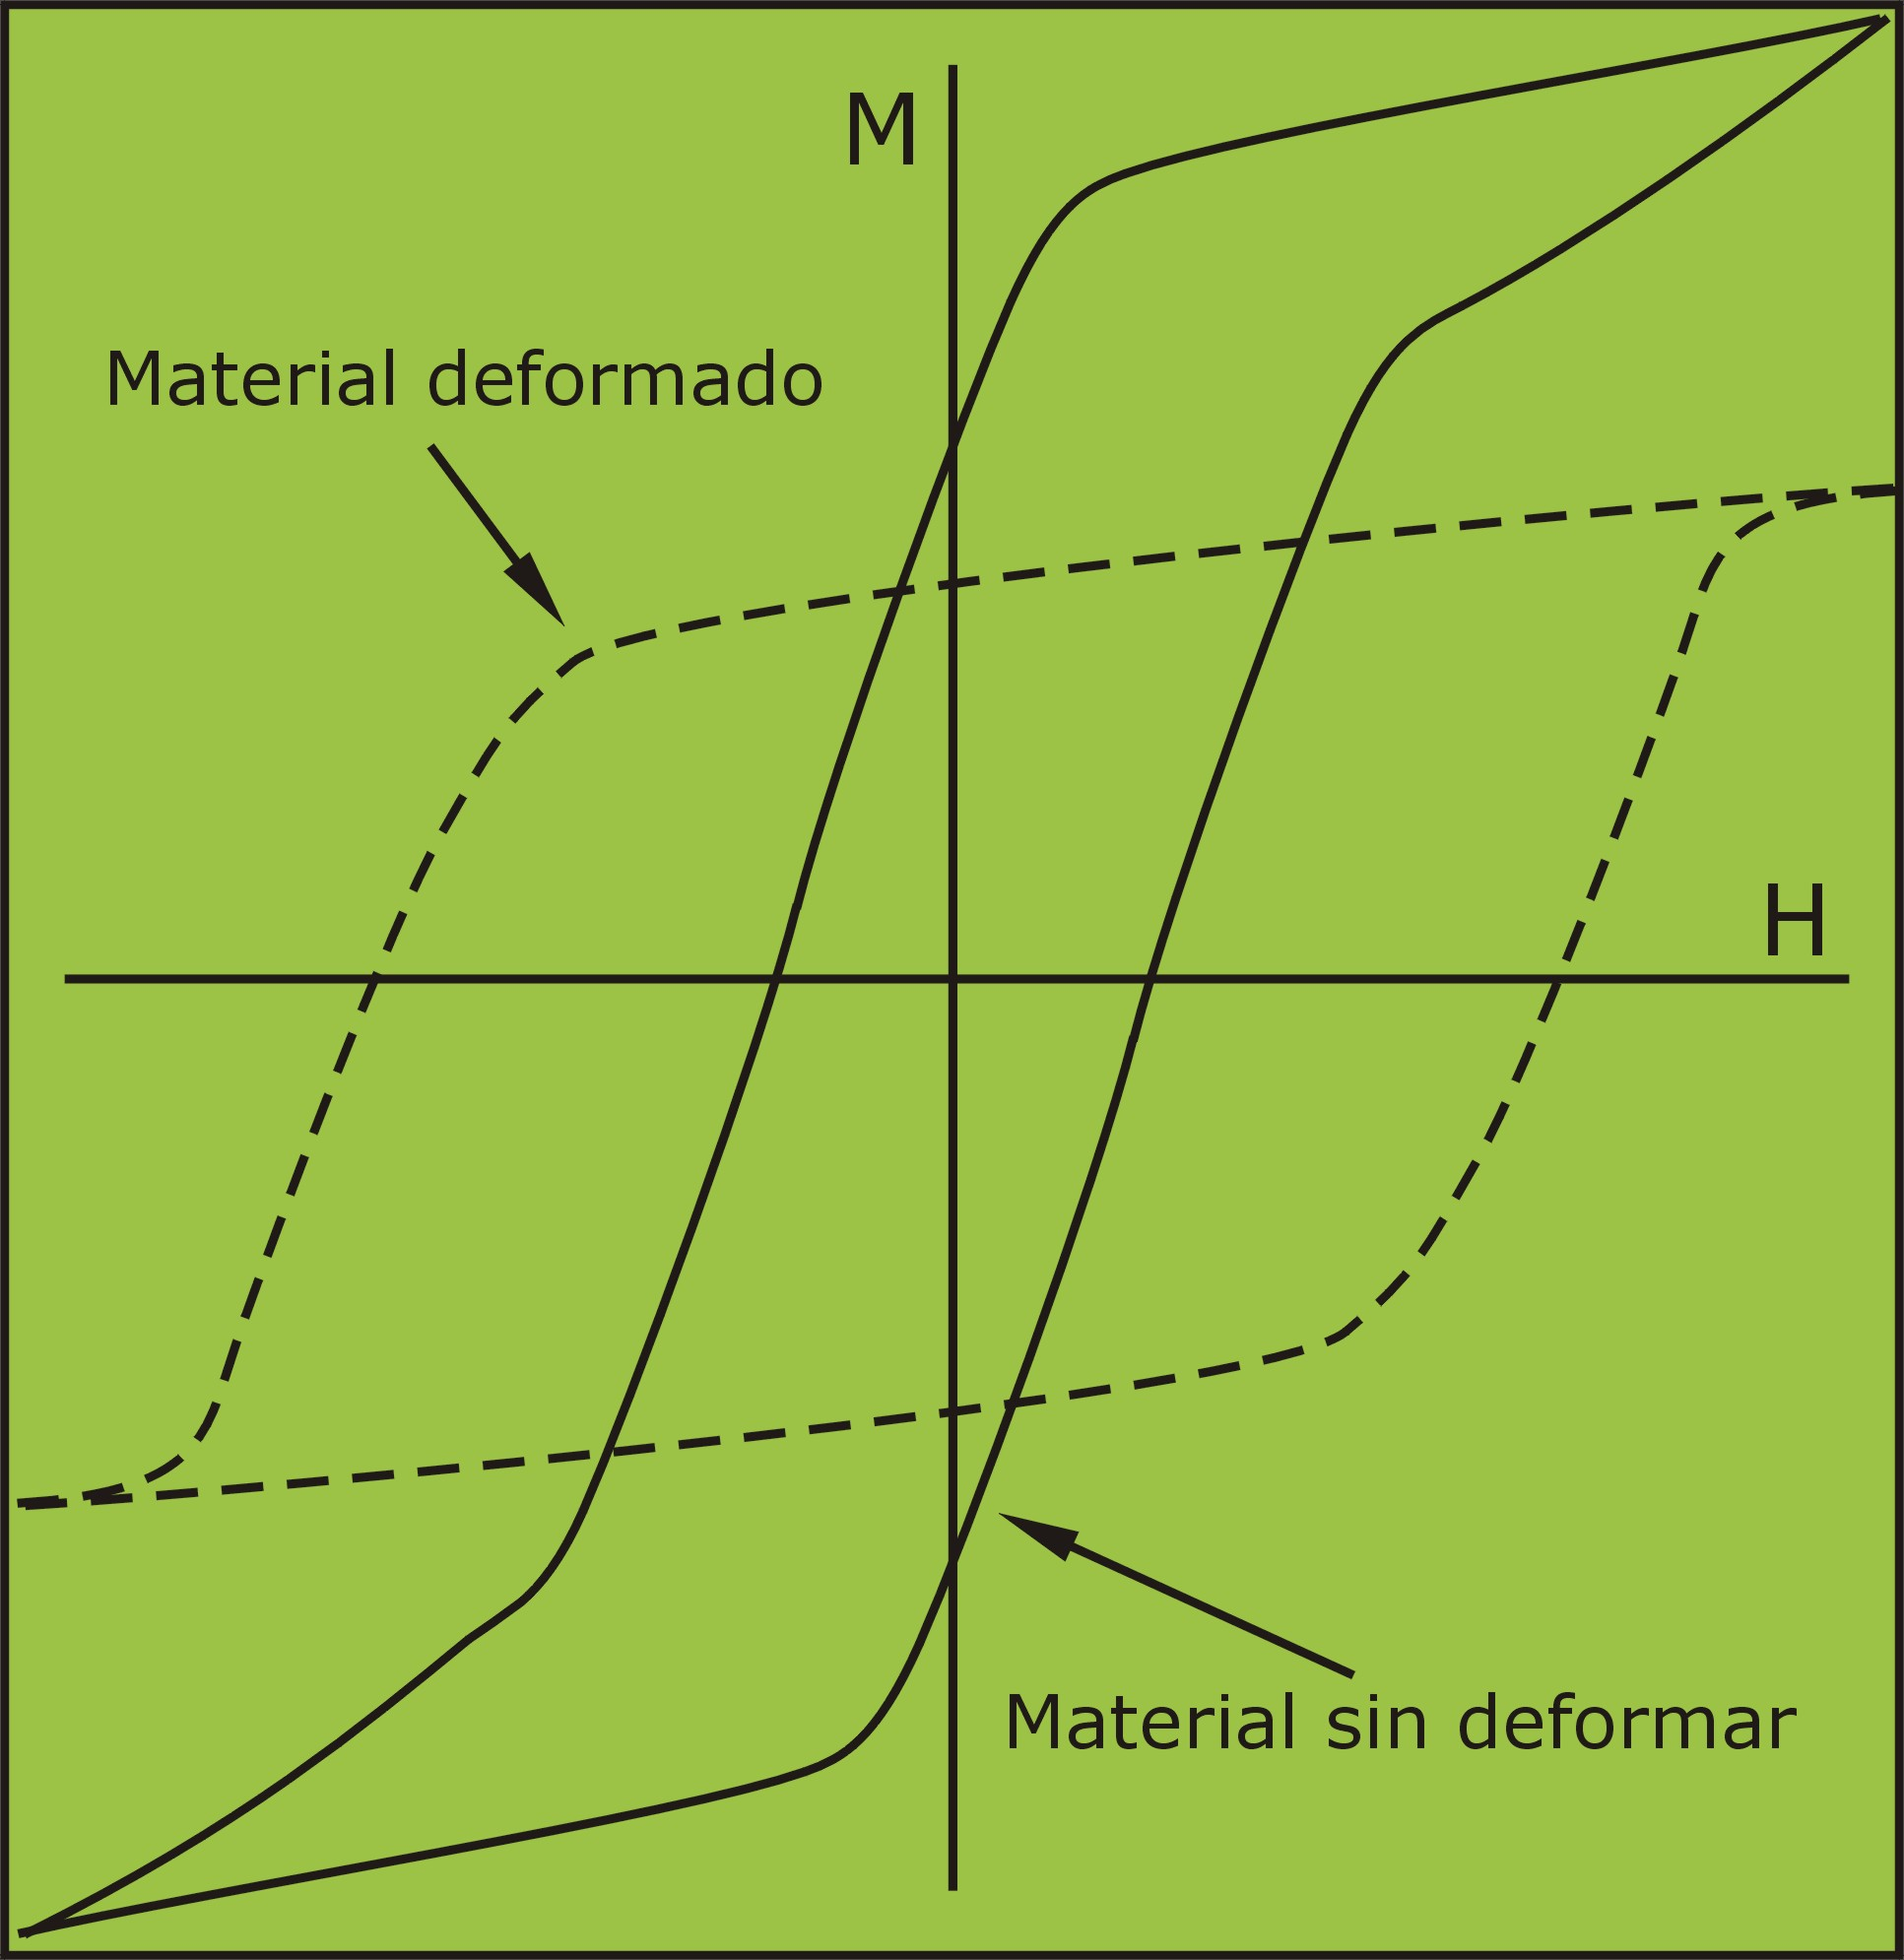
\includegraphics[width=0.6\textwidth]{./Figures/deformacionMecanica}
	\caption{Ciclo de histéresis para estados normal y deformado}
	\label{fig:deformacionMecanica}
\end{figure}


Mientras que en la figura \ref{fig:resistividad} observamos el cambio de la resistividad a $20C^{o}$ con el por ciento de aleante en el hierro, donde se destaca que el agregado de silicio disminuiría las corrientes parásitas.



\begin{figure}[H]
    \centering
    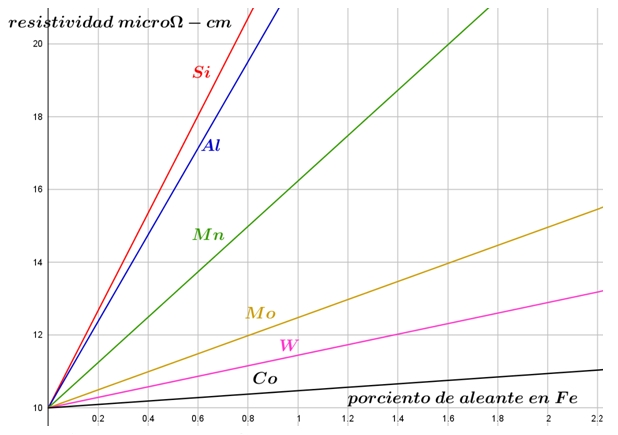
\includegraphics[width=1.0\textwidth]{./Figures/resistividad}
	\caption{Ciclo de histéresis para estados normal y deformado}
	\label{fig:resistividad}
\end{figure}

\subsection{Efecto del tamaño de grano del acero en las características magnéticas:}

	Existen expresiones aproximadas que me permiten calcular las pérdidas en el hierro (alta pureza y $B=1T$) en función del tamaño de grano del mismo (atención se trata del grano, no del dominio). El borde de grano actúa como zona de acumulación de impurezas y precipitados. 

\begin{figure}[H]
\begin{minipage}[b]{0.45\linewidth}
	\raggedright
    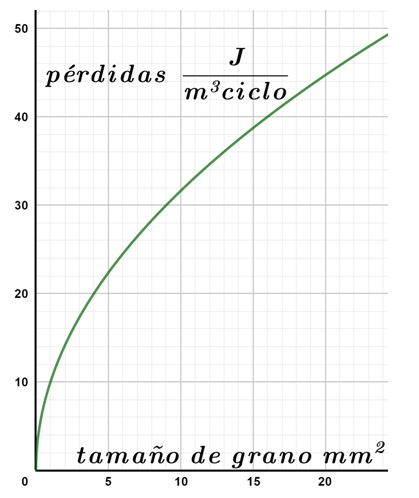
\includegraphics[width=1.0\textwidth]{./Figures/perdidasTamanhoGrano}
    \label{fig:perdidasTamanhoGrano}
\end{minipage}
\begin{minipage}[b]{0.50\textwidth}
	\vspace{0pt}
Por tanto es posible trabajar sobre los precipitados y tamaño de grano para obtener los resultados deseados. Si el material es fácilmente magnetizable estamos en presencia de un material magnéticamente blando, esto significa que los dominios magnéticos se pueden mover fácilmente. Por el contrario, si es difícil mover los limites de los dominios magnéticos, el material es magnéticamente duro y posee una fuerza coercitiva elevada. En algunos casos las paredes pueden estar totalmente inmovilizadas.

\vspace{1.2cm}
\end{minipage}
\end{figure}


De igual manera tenemos una expresión que permite estimar $H_{c}$ en función del tamaño de grano de la aleación, para un acero de alta pureza y $B=1T$. Similares relaciones se encuentran con el contenido de otros elementos, como azufre, oxígeno, etc. En definitiva encontramos parámetros, (para un dado material) 

\begin{figure}[H]
\begin{minipage}[b]{0.45\textwidth}
	\vspace{0pt}
del ciclo de histéresis que son efectivamente afectados por las propiedades metalúrgicas del material y otro paramentos que no lo son:
Son insensibles al cambio de la estructura la inducción de saturación y la temperatura de Curie, puesto que dependen básicamente de la composición química del material. 

Son sensibles a la estructura la fuerza coercitiva, la inducción remanente, permeabilidad y también el área del ciclo o sea la energía, prácticamente todos los parámetros que afectan el comportamiento duro o blando de un material.

\vspace{0.8cm}
\end{minipage}
\begin{minipage}[b]{0.50\linewidth}
	\raggedleft
    \includegraphics[width=1.1\textwidth]{./Figures/características}
    \label{fig:características}
\end{minipage}

\end{figure}

\section{Anisotropías magnéticas}

Se llama anisotropía magnética a la inhomogeneidad de alguna propiedad magnética, por ejemplo que la susceptibilidad magnética al ser medidas en diferentes direcciones del espacio sea distinta.

\begin{figure}[H]
    \centering
    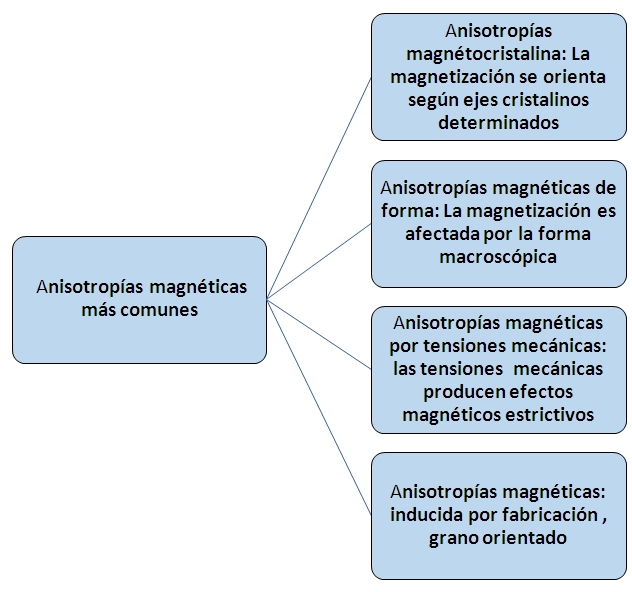
\includegraphics[width=0.8\textwidth]{./Figures/anhisotropiasMagneticas}
	\label{fig:anhisotropiasMagneticas.jpg}
\end{figure}


\subsection{Anisotropías magnétocristalinas}

\begin{itemize}
	\item Del estudio de la magnetización de materiales monocristalinos ferrosos se concluye que existen direcciones en las cuales es fácil magnetizar al monocristal y otras es más costoso (energéticamente hablando) hacerlo. Así, por ejemplo, en el hierro la dirección \textbf{[100]} es de fácil magnetización, mientras que la \textbf{[111]} es de difícil magnetización.

	\item La naturaleza de esta anisotropía puede ser entendida de la siguiente manera: la interacción de canje es culombiana y por tanto, isótropa, sin embargo, los momentos magnéticos no lo son necesariamente. La causa principal de anisotropía en el momento magnético es la relación entre el momento magnético de espín y el momento magnético orbital.
	
	\item En el esquema de la figura se observa la variación de la magnetización con el ángulo.
	
	
\begin{figure}[H]
    \centering
    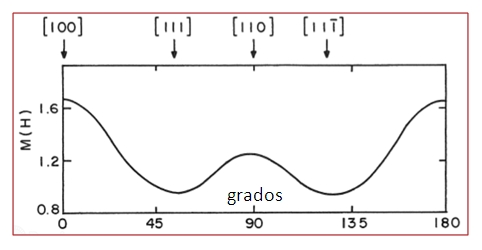
\includegraphics[width=0.8\textwidth]{./Figures/anhisotropiaMagnetocristalina}
	\caption{Anhisotropía magnetocristalina}
	\label{fig:anhisotropiaMagnetocristalina}
\end{figure}
	
	
	\item La dependencia de las propiedades magnéticas con la direcciones cristalográficas se llama anisotropía magnétocristalina.

\end{itemize}


En el esquema anterior, las seis direcciones equivalentes, se representan por la notación \textbf{[100]}. La dirección cristalográfica en la que se alcanza la saturación con el menor $H$ son las direcciones de fácil magnetización. Las direcciones de fácil magnetización son los ejes de magnetización espontánea de los dominios en ausencia de $H$.

Tomemos un simple ejemplo:

Supongamos un dipolo magnético en un metal y que sobre él actúa un campo $\vec{B}$, sabemos que el campo interactúa con el dipolo ($\vec{m}$) y producirá una variación de la energía:

\begin{equation}
\Delta E = -\vec{m} \cdot \vec{B}
\end{equation}

Luego la variación de la energía será:

\begin{equation}
\Delta E = -\mu_{0}\vec{m} \cdot (\vec{B} + \vec{M}) = -\mu_{0}\vec{m} \cdot \vec{B} -\mu_{0}\vec{m} \cdot \vec{M}
\end{equation}

Vemos que la variación de energía depende del campo externo $H$ y de $M$ o sea del material. Esta última expresión puede ser desarrollada como:

\begin{equation}
 -\mu_{0}\vec{m} \cdot \vec{M}  = -\mu_{0}m M Cos(\theta) = -\mu_{0}m M \left( 1-2 Sin^{2}\big(\mfrac {\theta}{2}\big) \right)  
\end{equation}

Vemos que hay un término que depende del ángulo que forma $m$ con $M$, esto nos indica que hay direcciones preferenciales de la estructura donde la energía será mínima $\theta = 0$. Este desarrollo elemental se verá ampliado más adelante


En los materiales ferromagnéticos policristalinos, los dominios con desiguales orientaciones llegan a saturación a diferentes intensidades de campo. En el $Co$, ver figura \ref{fig:policristalino2} todas las direcciones del plano basal normal al eje de fácil magnetización son direcciones de difícil magnetización.

\begin{figure}[H]
    \centering
    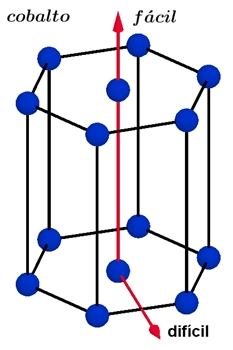
\includegraphics[width=0.3\textwidth]{./Figures/policristalino3}
	\caption{Cobalto}
	\label{fig:policristalino3}
\end{figure}

Hay direcciones cristalinas donde es fácil llegar a saturación, están son las dirección de fácil magnetización, saturando a bajos campos, mientras que los dominios orientados en las direcciones difíciles alcanzarán la saturación a campos mucho más altos En los esquemas se observa las direcciones de fácil y difícil magnetización para los tres materiales ferromagnéticos más comunes.

\begin{figure}[H]
  \centering
  \begin{minipage}[b]{0.47\textwidth}
    \raggedright
     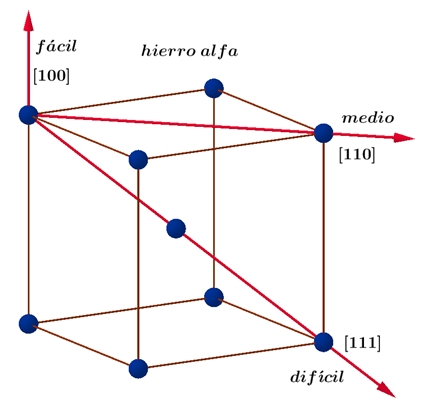
\includegraphics[width=1.10\textwidth]{./Figures/policristalino1}
  \end{minipage}
  \hfill
  \begin{minipage}[b]{0.47\textwidth}
    \raggedleft
     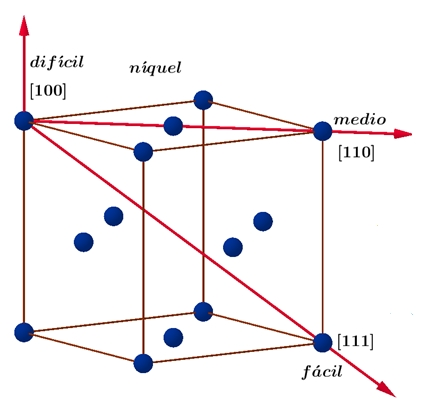
\includegraphics[width=1.10\textwidth]{./Figures/policristalino2}
  \end{minipage}
  \caption{Direcciones preferenciales Hierro $\alpha$ y Níquel}
\end{figure}

\subsection{Curvas de magnetización en función del campo}

En los grafico se observa la magnetización en función del campo magnético $H$, para tres elementos de transición $Fe$, $Ni$ y $Co$.

\begin{figure}[H]
    \centering
    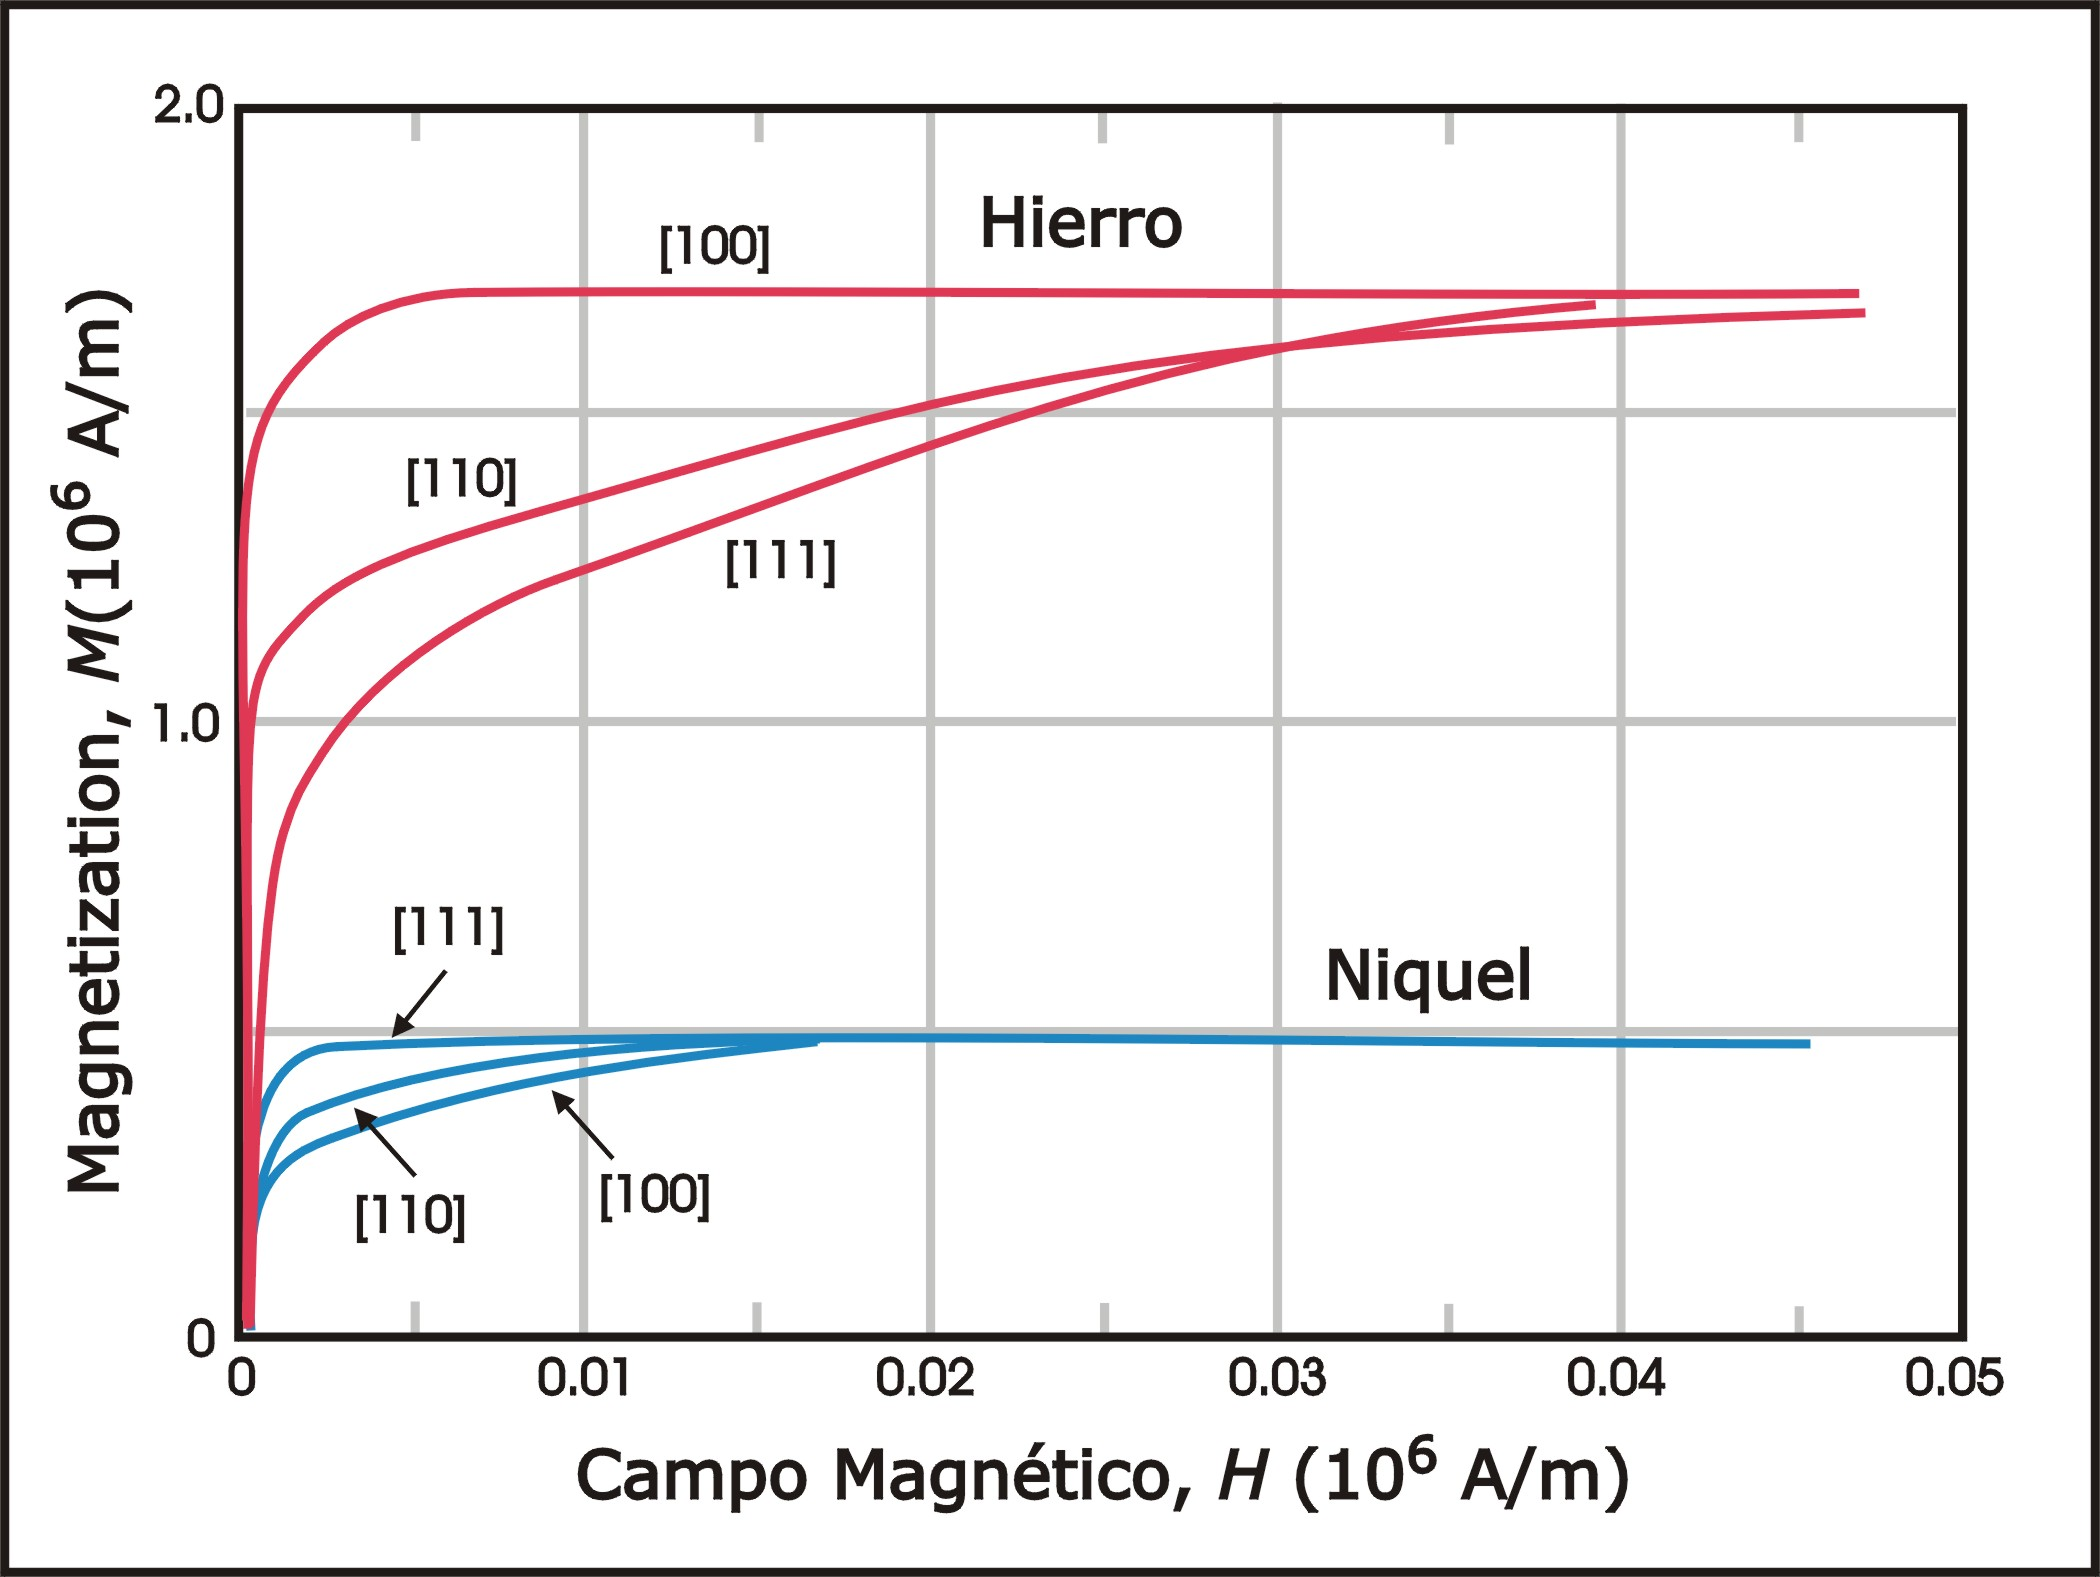
\includegraphics[width=0.8\textwidth]{./Figures/MagneticAnisotropy2}
	\caption{$Fe$ y $Ni$ Magnetización para direcciones preferenciales}
	\label{fig:MagneticAnisotropy2}
\end{figure}

Destacándose, en los de estructura cubica las tres direcciones de magnetización fácil \textbf{[100]} para el hierro y \textbf{[111]} para el níquel.

y en el cobalto que cristaliza como hexagonal, las dos direcciones de fácil (verde) y difícil  (marrón) magnetización.

\begin{figure}[H]
    \centering
    \includegraphics[width=0.8\textwidth]{./Figures/MagneticAnisotropy1}
	\caption{$Co$ Magnetización para direcciones preferenciales}
	\label{fig:MagneticAnisotropy1}
\end{figure}


\subsection{Energía de anisotropía}

Está claro que para magnetizar un material en una dirección se requiere una determinada energía. El trabajo realizado para rotar los dominios se denomina energía de anisotropía magnétocristalina.
\textbf{Akulov} en 1936 postuló una expresión para la energía de anisotropía, por unidad de volumen, para \textbf{cristales cúbicos}, cuando la magnetización de saturación $M-{s}$ forma ángulos $\alpha$, $\beta$, $\gamma$  con los ejes cristalinos, de la forma:


\begin{multline}
E=K_{0}+K_{1}(Cos^{2}(\alpha)Cos^{2}(\beta)+Cos^{2}(\beta)Cos^{2}(\gamma)+Cos^{2}(\gamma)Cos^{2}(\alpha)+ \\
k_{2}Cos^{2}(\alpha)Cos^{2}(\beta)Cos^{2}(\gamma)
\end{multline}

generalmente se desprecian los términos mayores a cuarto grado.

donde $K_{0}$, $K_{1}$ y $K_{2}$, son constantes que dependen del material y de la temperatura y están expresadas en ${\left[ \mfrac{erg}{cm^{3}}\right] }$. 

Para el $Fe$: ${K_{1}=44,8.10^{5}}$ y ${K_{2}=0,5.10^{5}}$, mientras que para el $Ni$: ${K_{1}=-0,5.10^{5}}$ y ${K_{2}=-0,2.10^{5}}$. 

$K_{0}$ es independiente del ángulo y como interesa la variación de la energía generalmente se lo desprecia.

La expresión de la energía cambia para el caso de cristales hexagonales, para el $Co$ y es:

\begin{equation}
E=K_{0}+K_{1}(Sin^{2}(\theta)+K_{2}Sin^{4}(\theta)+\cdots+
\end{equation}

Donde $\theta$ es el ángulo que $M_{s}$ forma con el eje de fácil magnetización. Donde ${K_{1} = 4,8.10^{6}}$ y ${K_{2} = 1,5.10^{6}}$

En el esquema de la figura \ref{fig:densidadEnergia1} vemos para un sistema cúbico la densidad de energía de anisotropía. En la figura de la Izquierda los ejes de coordenadas son ejes de fácil magnetización, si $K_{1}$ y $K_{2}$ son positivos (caso del $Fe$) se nota que la menor energía (azul) seis direcciones se obtiene cuando $M_{s}$ es paralelo a la dirección fácil \textbf{[100]} y mayor en la dirección difícil \textbf{[111]}. Por el contrario, cuando $K_{1}$ y $K_{2} < 0$ (caso  del $Ni$) surge una situación más compleja. Hay ocho mínimos (azul) a lo largo de las direcciones de los vértices del cubo (dirección \textbf{[111]}) y las direcciones de los ejes de coordenadas se convierten ahora en ejes de difícil magnetización.

\begin{figure}[H]
    \centering
    \includegraphics[width=1.0\textwidth]{./Figures/densidadEnergia1}
	\caption{Densidad de energia $Fe$}
	\label{fig:densidadEnergia1}
\end{figure}

Veamos en la figura \ref{fig:densidadEnergia2} el caso del $Co$, en la literatura científica se lo denomina anisotropía uniaxial.

En el Co comportamiento anisotrópico depende del signo de la constante $K_{1}$ cuando $K_{1}> 0$, la energía de anisotropía admite dos mínimos en $\theta=0$ y $\theta=\pi$, es decir cuando la magnetización se encuentra en la dirección $z$ positiva o negativa sin orientación preferencial (esquema de la izquierda). Este caso a menudo se conoce como anisotropía de fácil magnetización. Por el contrario, cuando $K_{1}<0$ la energía se minimiza para ${\theta=\mfrac{\pi}{2}}$, lo que significa un plano de fácil magnetización (esquema de la derecha).

\begin{figure}[H]
    \centering
    \includegraphics[width=1.0\textwidth]{./Figures/densidadEnergia2}
	\caption{Densidad de energia $Co$}
	\label{fig:densidadEnergia2}
\end{figure}


\section{Algo más sobre dominios magnéticos}

\begin{itemize}
	\item Con los conocimientos adquiridos, hasta aquí, podemos avanzar un poco más sobre los dominios
magnéticos. La energía necesaria para formar un dominio de cierre es la energía de anisotropía
cristalina que trata de alinearlos según las direcciones de fácil magnetización. Se requiere mayor energía si la dirección es un eje arbitrario.

	\item Como se vio el cobalto tiene un solo eje de fácil magnetización mientras que en el hierro, que es cubico, las aristas son los ejes de fácil magnetización, en el níquel que también tiene una estructura cubica, los ejes de fácil son las diagonales del cubo, luego en el Co si los dominios mayores están magnetizados en la dirección de fácil magnetización los de cierre deberán estar obligatoriamente en la dirección de difícil magnetización. En el caso del hierro es posible que ambos dominios de cierre y mayores estén magnetizados en direcciones, diferentes, de fácil magnetización.
	
	\begin{figure}[H]
    \centering
    \includegraphics[width=0.3\textwidth]{./Figures/cierre}
	\caption{Cierres magnéticos}
	\label{fig:cierre}
	\end{figure}

\end{itemize}


\subsection{Campo desmagnetizante}
$\centerdot$ Supongamos que tenemos una barra de un material ferromagnético, y que esta tiene una longitud mayor que las otras dos dimensiones, ver figura \ref{fig:}





\begin{figure}[H]
\begin{minipage}[b]{0.5\textwidth}
	\vspace{0pt}
$\centerdot$ Supongamos también que aplicamos un campo $H_{y}$ y otro perpendicular $H_{x}$, luego calculamos la magnetización en función del campo aplicado, ver figura Se observa que no son iguales, luego la forma de la curva de no solo depende de las propiedades magnéticas del mismo si no también de la forma de la muestra, algo similar sucede con la susceptibilidad.

\end{minipage}
\begin{minipage}[b]{0.45\linewidth}
	\raggedright
    \includegraphics[width=1.0\textwidth]{./Figures/campoDesmagnetizante0}
    \vspace{0.5cm}
\end{minipage}

\end{figure}


\begin{figure}[H]
\begin{minipage}[b]{0.5\linewidth}
	\raggedright
    \includegraphics[width=0.8\textwidth]{./Figures/campoDesmagnetizante1}

\end{minipage}
\begin{minipage}[b]{0.45\textwidth}
	\vspace{0pt}
$\centerdot$ Cuando el campo se aplica en la dirección de $x$, los polos inducidos están más separados y el campo desmagnetizarte es menor. Cuando el mismo campo externo se aplica a lo largo de $y$, los polos estarán más cercanos y el campo desmagnetizaste será mayor.
    \vspace{2.5cm}
\end{minipage}
\end{figure}

\subsection{Anisotropías magnéticas de forma}

La magnetización se ve afectada por la forma macroscópica del sólido. Muestras policristalinas, sin una orientación preferida de los granos, no tienen ninguna anisotropía magneto-cristalina, su comportamiento es magnéticamente isotrópico solamente para una forma esférica. Si se magnetiza una muestra se formaran polos en los extremos que provocan un campo, como ya fue visto, desmagnetizarte dentro del material. El campo desmagnetizarte es proporcional a la magnetización que lo origina:

\begin{equation}
	\overrightarrow{H_{d}}= -N \overrightarrow{M}
\end{equation}

Siendo $N$ el tensor desmagnetizante.

El cálculo es bastante complicado en su forma general, por lo que se lo hace para geometrías regulares:


\begin{figure}[H]
    \centering
    \includegraphics[width=0.8\textwidth]{./Figures/anisotropiasDeForma}
	\caption{Anisotropias de forma}
	\label{fig:anisotropiasDeForma}
\end{figure}

\begin{equation}
	E=K_{0}+K_{1} Sin^{2}(\alpha)
\end{equation}

Donde $K_{0}= M^{2}\mfrac{N_{b}}{2}$ y $K_{1}=(N_{a}-N_{b})-\mfrac{M^{2}}{2}$, $E$ es la energía de anisotropía, $N_{a}$ y $N_{b}$ son las constantes de desmagnetización para los ejes $a$ y $b$

\section{Anisotropía magnéticas por tensión, Magnetostricción}

\begin{itemize}
	\item Es la propiedad que tienen los materiales ferromagnéticos de cambiar de tamaño en presencia de un campo magnético. Por ejemplo el $Ni$ al colocarlo en campo magnético se contrae en la dirección del campo y se dilata en la dirección Transversal.
	
	\item \textbf{Joule} observó la magnetostricción por primera vez en 1842, por eso es llamada magnetostricción de joule.
	
	\item Un material magnetostrictivo modifica sus dimensiones si el campo cambia. También es un fenómeno reversible, si aplicamos una tensión mecánica cambia su estado magnético, llamado
efecto \textbf{Villari} o efecto magnetostrictivo inverso.

	\item Dos procesos pueden explicar la magnetostricción: la migración de las paredes del dominio dentro del material en respuesta a campos magnéticos externos y la rotación de los dominios. Estos dos mecanismos permiten que el material cambie la orientación del dominio, lo que a su vez provoca un cambio dimensional. Permaneciendo el volumen constate, luego la otra dimensión del cuerpo debe tener una contracción.
	
	
	\begin{figure}[H]
    \centering
    \includegraphics[width=0.5\textwidth]{./Figures/magnetostriccion}
	\caption{Magnetostriccion}
	\label{fig:magnetostriccion_1}
	\end{figure}
	
	\item Se llama constante de magnetostricción a $\lambda$ cuyo valor es: $\lambda=\mfrac{\Delta l}{l}$
	El cambio relativo $\lambda$ puede ser $\lambda> 0$ o $\lambda< 0$ donde $\Delta l$ es la variación de la longitud y $l$ la longitud inicial. Ver en la figura \ref{fig:magnetostriccion} la reorientación de los dominios. Hay dos tipos de magnetostricción: espontaneo y forzado. El primero ocurre cuando enfriamos el material por debajo de $T_{c}$ y la segunda cuando tratamos de reorientar los dominios que se generados espontáneamente.
\end{itemize}

\subsection{Magnetostricción en saturación}

El valor de $\lambda$ medido en saturación lo llamamos $\lambda_{s}$ (magnetostricción en saturación), en el gráfico se muestra la variación de $\lambda$ en función del campo $H$ para un material con $\lambda> 0$, observamos que cuando el campo es pequeño $\lambda$ aumenta poco, posteriormente se incrementa $\lambda$ llegando a saturación $\lambda_{s}$. Los valores de $\lambda$ mayores a $\lambda_{s}$ se llama magnetostricción forzada $\lambda_{f}$ y son muy bajos.

\begin{figure}[H]
    \centering
    \includegraphics[width=0.8\textwidth]{./Figures/magnetoestriccion}
	\caption{Saturación en magnetoestriccion}
	\label{fig:magnetoestriccion_2}
\end{figure}

Como el volumen del material permanece constante durante el aumento de $H$ se puede pensar que la magnetostricción longitudinal es:

\begin{equation}
	\lambda_{t} = \mfrac{-\lambda}{2}
\end{equation}

Si observamos la figura \ref{fig:magnetoestriccion} vemos que una parte importante de la gráfica puede aproximarse a una recta, esto significa que una variación de $H$ generara una $\lambda$ proporcional, estamos frente al principio de un traductor magnetostrictivo reversible. El estado de saturación se encuentra perfectamente definido, consiste de un solo dominio con un $M_{s}$ en la dirección del campo aplicado, por el contrario, el estado desmagnetizado inicial no está bien definido.

\subsection{Magnetostricción en monocristales cúbicos}

El mecanismo de magnetostricción es la deformación entre el estado desmagnetizado y el de
saturación. Se observa que el estado de saturación es único (bien definido) y se accede cuando todos los dominios están en la misma dirección. En contraposición el estado inicial desmagnetizado no es único hay varias maneras de obtener un estado de desmagnetización. El caso de monocristales cúbicos: la ecuación que veremos se basa en una definición arbitraria del estado inicial desmagnetizado “todos los posibles tipos de dominios tienen igual volumen” y otras arbitrariedades. Estas diferencias generan arbitrariedades en distintos trabajos, los mismos no parten de iguales condiciones Iniciales.


\begin{figure}[H]
    \centering
    \includegraphics[width=0.8\textwidth]{./Figures/monocristalesCubicos}
	\caption{monocristalesCubicos}
	\label{fig:monocristalesCubicos}
\end{figure}


En la ecuación \ref{eq:magnetoestriccion} tenemos la expresión de la constante de magnetostricción $\lambda_{s}$ para un mono cristal cubico, téngase en cuenta que es aproximada, no obstante las aproximaciones no son significativas. Si tenemos un mono cristal
saturado en una dada dirección, donde $\alpha_{1}$, $\alpha_{2}$, $\alpha_{3}$, son los cosenos directores de esa dirección, respecto a los ejes de la estructura cubica. Se puede conocer la deformación en otra dirección, dada por los cosenos directores $\beta_{1}$, $\beta_{2}$, $\beta_{3}$, mientras que $\lambda_{100}$ y $\lambda_{111}$, representan el cambio de longitud en saturación en las direcciones \textbf{[100]} y \textbf{[111]}, respectivamente.

\begin{multline}
	\lambda_{s}=\mfrac{\Delta l}{l}=\mfrac{3}{2}\lambda_{100}\big(\alpha_{1}^{2}\beta_{1}^{2}+
	\alpha_{2}^{2}\beta_{2}^{2}+\alpha_{3}^{2}\beta_{3}^{2}-\mfrac{1}{3} \big)+\\
	3\lambda_{111}\big(\alpha_{1}\alpha_{2}\beta_{1}\beta_{2}+
	alpha_{3}\alpha_{2}\beta_{3}\beta_{2}+\alpha_{1}\alpha_{3}\beta_{1}\beta_{3} \big)
	\label{eq:magnetoestriccion1}
\end{multline}

\subsection{Magnetostricción y estado inicial}

$\centerdot$Veamos un ejemplo donde queda clara la dependencia de la magnetostricción, con el estado inicial desmagnetizado. Esto de alguna manera justifica las diferencias encontradas por distintos investigadores al realizar un mismo ensayo, ya que no podemos establecer fehacientemente las condiciones iniciales. Existen una infinidad de estados desmagnetizados.

$\centerdot$Los dominios vecinos con magnetización opuesta no poseen energía elástica, puesto que en ellos $\lambda$ es igual. Por tanto el movimiento de las paredes de $180^{o}$ no implica cambios en las dimensiones. Por el contrario el movimiento de las paredes de $90^{o}$ si implica cambios en las dimensiones


\begin{figure}[H]
    \centering
    \includegraphics[width=0.8\textwidth]{./Figures/estadoInicial}
	\caption{Magnestoestricción y estado inicial}
	\label{fig:estadoInicial}
\end{figure}

\subsection{Magnetostricción en monocristales cúbicos}

Veamos el caso en que se desea hallar la deformación cuando esta coincide con la dirección de la magnetización, luego los ángulos son iguales, por tanto $\alpha_{1}=\beta_{1}$, $\alpha_{2}=\beta_{2}$, $\alpha_{3}=\beta_{3}$.

\begin{multline}
	\lambda_{s}=\mfrac{\Delta l}{l}=\mfrac{3}{2}\lambda_{100}\big(\alpha_{1}^{2}\beta_{1}^{2}+
	\alpha_{2}^{2}\beta_{2}^{2}+\alpha_{3}^{2}\beta_{3}^{2}-\mfrac{1}{3} \big)+\\
	3\lambda_{111}\big(\alpha_{1}\alpha_{2}\beta_{1}\beta_{2}+
	\alpha_{3}\alpha_{2}\beta_{3}\beta_{2}+\alpha_{1}\alpha_{3}\beta_{1}\beta_{3} \big)= \\
	\mfrac{3}{2}\lambda_{100}\big(\alpha_{1}^{4}+\alpha_{2}^{4}+\alpha_{3}^{4}-\mfrac{1}{3} \big)+
	3\lambda_{111} \big( \alpha_{1}^{2} \alpha_{2}^{2} + \alpha_{3}^{2} \alpha_{2}^{2} + \alpha_{1}^{2}\alpha_{3}^{2} \big)
	\label{eq:magnetoestriccion2}
\end{multline}

Como: ${\big(\alpha_{1}^{2}+\alpha_{2}^{2}+\alpha_{3}^{2} \big)^2 = 1 = \big(\alpha_{1}^{4}+\alpha_{2}^{4}+\alpha_{3}^{4}\big)+2\big( \alpha_{1}^{2} \alpha_{2}^{2} + \alpha_{3}^{2} \alpha_{2}^{2} + \alpha_{1}^{2}\alpha_{3}^{2} \big)}$, reemplazando y operando llegamos a que:

\begin{equation}
\lambda = \lambda_{100}+3(\lambda_{111}-\lambda_{100})\big( \alpha_{1}^{2} \alpha_{2}^{2} + \alpha_{3}^{2} \alpha_{2}^{2} + \alpha_{1}^{2}\alpha_{3}^{2} \big)
\end{equation}

\textbf{Otro caso:} si bien la ecuación que nos da $\lambda_{s}$ es empírica y depende del estado inicial, generalmente incierto, es de utilidad como una primera aproximación. La podemos utilizar para calcular el cambio de dimensión de
un mono dominio debido a la rotación de su vector $M_{s}$ fuera de la dirección de fácil magnetización. Si calculamos el valor de $\lambda_{s}$ para dos orientaciones diferentes de $M_{s}$, en saturación, entonces la diferencia de dichos valores es la deformación. Supongamos que $M_{s}$ rota alrededor del eje \textbf{[001]} un ángulo $\delta$ estado en el plano \textbf{[010]} . Entonces, los cosenos directores de $M_{s}$ serán por tanto $\alpha_{1} = Cos(90 – \delta) = Sin(\delta), \alpha_{2} = 0, \alpha_{3} = Cos(\delta)$, y como queremos conocer la deformación en la dirección \textbf{[001]} los cosenos directores quedan, $\beta_{1} = 0$, $\beta_{2} = 0$, y $\beta_{3} = 1$ reemplazando queda:

\begin{equation}
\lambda(\delta) = \mfrac{\Delta l}{l}=\mfrac{3}{2}\lambda_{100} \big( Cos^{2}(\delta)-\mfrac{1}{3} \big) \text{, que es la deformación a lo largo \textbf{[001]} }
\end{equation}



\begin{figure}[H]
    \centering
    \includegraphics[width=0.4\textwidth]{./Figures/magnetoestriccionCubicos}
	\caption{Magnetoestriccion cristales cúbicos}
	\label{fig:magnetoestriccionCubicos}
\end{figure}


La expresión se reduce cuando $\delta=0$ a ${\lambda(\delta = 0) = \lambda_{100}}$. Si tomamos el estado de saturación a lo largo de \textbf{[001]} como estado inicial, luego


\begin{multline}
\lambda_{s} = \mfrac{\Delta l}{l}=\lambda(\delta)-\lambda(0)= \mfrac{3}{2}\lambda_{100} \big( Cos^{2}(\delta)-\mfrac{1}{3} \big) - \lambda_{100} = \\
\mfrac{3}{2}\lambda_{100} Cos^{2}(\delta)- \mfrac{1}{2}\lambda_{100} - \lambda_{100} =
\mfrac{3}{2}\lambda_{100} \big( Cos^{2}(\delta)- 1 \big) = \\
-\mfrac{3}{2}\lambda_{100} Sin^{2}(\delta)
\end{multline}


Cuando $M_{s}$ rota un ángulo de $90^{o}$ alejándose de la dirección de fácil magnetización el dominio se contrae $\mfrac{3}{2}\lambda_{100}$. El resultado muestra que las constantes de magnetostricción se pueden determinar experimentalmente sin importar el estado magnético inicial, que como se comento existen infinidad de estado. La idea es efectuar medidas de deformación con galgas extensiométricas, cuando $M_{s}$ rota de una
orientación a otra en condiciones de saturación.



Otro caso: Si el campo magnetizante está en la dirección de $x$ y medimos $\lambda$ en la dirección $z$, ${\alpha_{1} = \beta_{3}}$ y ${\alpha_{2} = \beta_{2} = \alpha_{3} = \beta_{1} = 0}$, luego:

\begin{equation}
\mfrac{3}{2}\lambda_{100}\big(-\mfrac{1}{3}\big) = - mfrac{\lambda_{100}}{2}
\end{equation}


Como se indica en la figura \ref{fig:magnetoestriccionOtroCaso} el signo $-$ menos indica contracción.

\begin{figure}[H]
    \centering
    \includegraphics[width=0.6\textwidth]{./Figures/magnetoestriccionOtroCaso}
	\caption{Magnetoestriccion cruzada}
	\label{fig:magnetoestriccionOtroCaso}
\end{figure}



\subsection{Magnetostricción de un material isótropo}
Supongamos que tenemos una partícula de estructura cúbica e isótropa lo cual significa que:

\begin{equation}
\lambda_{100}=\lambda_{111}=\lambda_{s}
\end{equation}

tendremos que la ecuación \ref{eq:magnetoestriccion2} se convertirá en:

\begin{equation}
	\lambda_{s}=\mfrac{\Delta l}{l}=\mfrac{3}{2}\lambda_{s} \big[ \big(\alpha_{1}\beta_{1}+ \alpha_{2}\beta_{2}+\alpha_{3}\beta_{3} \big)^{2} -\mfrac{1}{3} \big] 
		\label{eq:magnetIsot}
\end{equation}

La expresión de la ecuación \ref{eq:magnetIsot} es la del trinomio al cuadrado. Luego tenemos los productos de los cosenos directores de dos vectores con el mismo punto de aplicación, esto es igual al coseno del ángulo que forman los vectores ${Cos(\theta) = \big(\alpha_{1}\beta_{1}+ \alpha_{2}\beta_{2}+\alpha_{3}\beta_{3} \big)}$. Dicho de otro modo $\theta$ es el ángulo que forma la dirección en la que se quiere medir la magnetostricción ($\lambda_{\theta}$) y la dirección de magnetización.

\begin{equation}
	\lambda_{\theta}=\mfrac{3}{2}\lambda_{s} \big( \big( Cos^{2}(\theta)-1 \big) 
	\label{eq:magnetIsot2}
\end{equation}

\begin{figure}[H]
    \centering
    \includegraphics[width=0.5\textwidth]{./Figures/magnetoestriccionOtroCasoMas}
	\caption{Cristales cúbicos, dirección $\theta$}
	\label{fig:magnetoestriccionOtroCasoMas}
\end{figure}

\subsection{Magnetoestricción en cristales uniaxiales, (hexagonal)}

En este caso la expresión para un cristal hexagonal (cobalto) es:

\begin{multline}
\lambda = \lambda_{A} \big[ \big( \alpha_{1}\beta_{1}+\alpha_{2}\beta_{2}\big)^{2}-\big( \alpha_{1}\beta_{1}+\alpha_{2}\beta_{2}\big)\alpha_{3}\beta_{3}\big] + \\
\lambda_{B} \big[ \big(1- \alpha_{3}^{2}\big)\big(1-\beta_{3}^{2}\big)-\big( \alpha_{1}\beta_{1}+\alpha_{2}\beta_{2}\big)^{2} \big] + \\
\lambda_{C} \big[ \big( 1- \alpha_{3}^{2}\big)\beta_{3}^{2}-\big( \alpha_{1}\beta_{1}+\alpha_{2}\beta_{2}\big)\alpha_{3}\beta_{3} \big] + \\
4\lambda_{D} \big( \alpha_{1}\beta_{1}+\alpha_{2}\beta_{2}\big)\alpha_{3}\beta_{3}
	\label{eq:magnetostriccionUniaxiales}
\end{multline}

Los coeficientes en la ecuación \ref{eq:magnetostriccionUniaxiales} son:
$\alpha_{i}$: cosenos directores de la dirección de saturación respecto a los ejes de coordenadas.
$\beta_{i}$: cosenos directores de la dirección en la que se mide la magnetostricción respecto a los ejes de coordenadas.
$a_{1}$, $a_{2}$, $a_{3}$, $c$: son los ejes que habitualmente se utilizan en el sistema hexagonal.
Esta expresión es una primera aproximación e involucra a cuatro constantes y solamente es válida para cristales donde el eje de fácil magnetización es $c$

\begin{figure}[H]
    \centering
    \includegraphics[width=0.4\textwidth]{./Figures/MagnetoestriccionEnCristalesUniaxiales}
	\caption{Sistema de coordenadas, cristal hexagonal}
	\label{fig:MagnetoestriccionEnCristalesUniaxiales}
\end{figure}


El eje de fácil coincide con la coordenada $z$ y con $c$ Para el cobalto las constantes valen:

\begin{equation}
\begin{aligned}
	\lambda_{A} = -45.10^{-6} \quad \lambda_{B} = -95.10^{-6} \\
	\lambda_{A} = +110.10^{-6} \quad \lambda_{B} = -100.10^{-6} 
\end{aligned}
\end{equation}

Generalmente las constantes de magnetostricción decrecen en valor absoluto cuando la temperatura se incrementa y son $0$ a la temperatura de Curie.

$\centerdot$ Veamos el caso en que la magnetostricción es medida en la misma dirección que la magnetización, o sea



\begin{equation}
	\alpha_{1}= \beta_{1}, \; \alpha_{2}= \beta_{2}, \; \alpha_{3}= \beta_{3}
\end{equation}

En este caso, como ${\alpha_{1}^{2}+\alpha_{2}^{2}+\alpha_{3}^{2}=1}$ tomando la ecuación \ref{eq:magnetostriccionUniaxiales} trabajando sobre cada sumando tenemos que:

Queda entonces:

\begin{equation}
	\lambda = \lambda_{A} \big[\big(1-\alpha_{3}^{2}\big)^{2}-\big(1-\alpha_{3}^{2}\big)\alpha_{3} \big] + 4\lambda_{D} \big(1-\alpha_{3}^{2}\big)\alpha_{3}
\end{equation}

Observamos que la expresión para la magnetostricción depende solo de $\alpha_{3}$ independientemente de la dirección que elijamos en el plano basal, consecuencia de la simetría hexagonal.

\subsection{Anisotropía magnéticas por tensión: Magnetostricción}

El esquema que se visualiza a mas abajo nos muestra, el resultado experimental, de la variación de $\lambda$ con la magnetización para un monocristal de $Fe$, cortado en forma de rodaja cilíndrica.

$\centerdot$ Caso \textbf{[100]} campo en dirección \textbf{[100]}. En mono cristales, generalmente los dominios esta imanados en la dirección de fácil magnetización, hasta saturación. Debido a la magnetostricción, y como $\lambda>0$ , estos dominios están alargados según esta dirección. Si el campo $H$ coincide con \textbf{[100]} , entonces deben estar comprimidos en la direcciones transversales \textbf{[010]} y \textbf{[001]}. Como muestra la figura \ref{} la magnetostricción en esa dirección es siempre una expansión (marrón). Por esta razón podemos suponer que los dominios magnéticos en un material desmagnetizado están espontáneamente magnetizados en las direcciones \textbf{[100]} Muestra también que con campos pequeños se logra movimientos de dominios.



\begin{figure}[H]
    \centering
    \includegraphics[width=0.9\textwidth]{./Figures/hierroMonocristal}
	\caption{Magnetoestricción $Fe$ monocristal}
	\label{fig:hierroMonocristal}
\end{figure} 

$\centerdot$ Caso \textbf{[110]} campo en dirección \textbf{[110]}. En este caso el cristal primero se expande y luego se contrae.


$\centerdot$ Caso \textbf{[111]} campo en dirección \textbf{[111]}. Primero crecen los dominios \textbf{[$\ddot{1}$00]}, \textbf{[0$\ddot{1}$0]}y \textbf{[00$\ddot{1}$]} a expensas de los \textbf{[100]}, \textbf{[010]}y \textbf{[001]} respectivamente, aquí el movimiento de las paredes es de $180^{o}$, por tanto no altera las
dimensiones. En este estado $M_{s}$ en cada dominio forma un ángulo de $54,74^{o}$ con el campo. El aumento ulterior del campo produce rotaciones de los vectores magnetización hacia la dirección del campo lo cual da como resultado una contracción del cristal en la dirección \textbf{[111]} (azul).
Tratemos de justificar el comportamiento de estos tres casos, primero con un esquema para visualizarlo y luego formalmente, comencemos por: 

$\centerdot$ Caso \textbf{[111]}: En los esquemas observamos como se modifica los dominios al crecer el campo externo, no se representa cambio de longitud con el aumento del campo externo. El grupo de vectores en el origen simbolizan los vectores de fácil magnetización en el inicio, en cada dominio.



\begin{figure}[H]
    \centering
    \includegraphics[width=1.0\textwidth]{./Figures/anisotropiasPorTension1}
	\caption{Anisotropias por tension \textbf{[111]} }
	\label{fig:anisotropiasPorTension1}
\end{figure}

$\centerdot$ Caso \textbf{[110]}: El esquema que utilizamos aquí es distinto al anterior, representa un trozo del monocristal con forma de disco, en el suponemos cuatro dominios iniciales. En el plano \textbf{[001]}$= 0$, suponiendo también que cada dominio se encuentra espontáneamente magnetizados en las direcciones \textbf{[100]}. El campo magnético externo está en la dirección \textbf{[110]}.


\begin{figure}[H]
    \centering
    \includegraphics[width=1.1\textwidth]{./Figures/anisotropiasPorTension2}
	\caption{Anisotropias por tension \textbf{[110]}}
	\label{fig:anisotropiasPorTension2}
\end{figure}

$\centerdot $ Caso \textbf{[111]}: En este caso la representación es un cubo donde la diagonal es la dirección de $H$, \textbf{[111]}, que forma un ángulo de $57,74^{o}$ con las aristas del cubo, se observa también la dirección de $M_{s}$ en ese dominio. Los diferentes colores de los planos identifican a los que pasan por la base y el perpendicular a este que pasa por la diagonal y contiene a $M_{s}$ y a $H$.

\begin{figure}[H]
    \centering
    \includegraphics[width=0.5\textwidth]{./Figures/anisotropiasPorTension3}
	\caption{Anisotropias por tension \textbf{[111]}}
	\label{fig:anisotropiasPorTension3}
\end{figure}

Calculemos el $\lambda$ en cada uno de los casos anteriores, para ello utilizamos la expresión:

\begin{equation}
\lambda_{s}= \lambda_{100} + 3 (\lambda_{111} - \lambda_{100})(\alpha_{1}^{2}\alpha_{2}^{2}+\alpha_{2}^{2}\alpha_{3}^{2}+\alpha_{3}^{2}\alpha_{1}^{2})
\end{equation}

$\centerdot$ Caso \textbf{[100]}: Aquí salvo $\alpha_{1}$ el resto vale cero luego queda $\lambda_{s}= \lambda_{100} = +21.10^{-6}$

$\centerdot$ Caso \textbf{[110]}: En este caso los vectores se encuentran en el plano y solo es cero $\alpha_{3}$ quedando:

\begin{multline}
\lambda_{s}= 
\lambda_{100} + 3 (\lambda_{111} - \lambda_{100})(\alpha_{1}^{2}\alpha_{2}^{2})=
\lambda_{100} + 3 (\lambda_{111} - \lambda_{100})\alpha_{1}^{4}= \\
\lambda_{100} + 3 (\lambda_{111} - \lambda_{100})(\mfrac{\sqrt{2}}{2})^{4}=
\lambda_{100} + \mfrac{3}{4} (\lambda_{111} - \lambda_{100})
\end{multline}


Pero $\lambda_{111}=-\lambda_{100}$ por lo tanto

\begin{equation}
- \mfrac{1}{4} \lambda_{111} + \mfrac{3}{4}\lambda_{111}= -\mfrac{\lambda_{111}}{2} = -10,5.10^{-6}
\end{equation}

que da negativo y menor como se puede ver en la figura \ref{fig:anisotropiasPorTension2}

$\centerdot$ Caso \textbf{[111]}: En este caso, como se puede ver nuevamente en la figura \ref{fig:anisotropiasPorTension2}, el ángulo vale $57,74^{o}$, luego la expresión queda:

\begin{equation}
\lambda_{s}= \lambda_{100} + 3 (\lambda_{111} - \lambda_{100})(3 \alpha_{1}^{4})
\end{equation}

Pero ${\alpha =  Sin(57.74^{o}) = \mfrac{1}{\sqrt{3}}}$ por tanto:

\begin{equation}
\lambda_{s}= 
\lambda_{100} + 3 (\lambda_{111} - \lambda_{100})(\mfrac{1}{\sqrt{3}})^{4}=
\end{equation}

Dando negativo como se observó experimentalmente

\begin{figure}[H]
    \centering
    \includegraphics[width=1.1\textwidth]{./Figures/fenomenosMagnetoestrictivos}
	\caption{Síntesis de fenomenos magnetoestrictivos}
	\label{fig:fenomenosMagnetoestrictivos}
\end{figure}


\subsection{Breve historia de la magnetostricción}

\begin{itemize}
	\item 1847 el escocés \textbf{James Joule} descubre la magnetoestricción en el Fe. También describió el fenómeno inverso de la magnetostricción, una verdadera hazaña en aquella época, pues la deformación es de pocas partes por millón.
	
	\item 1865 \textbf{Villari} caracteriza el fenómeno inverso (cambio del estado de magnético cuando se le aplica un esfuerzo mecánico. (efecto Villari).
	
	\item 1862 \textbf{Wiedemann} descubre el efecto que lleva su nombre, torsión de un material magnetoestrictivo al aplicarle simultáneamente un campo axial y otro circunferencial.
	
	\item 1882 \textbf{Barret} observó que, al contrario del Fe, el Ni se contrae al aplicarle un campo magnético. También observo cambios de volumen.

	\item 1886 \textbf{Bidwell} encontró que a campos muy intensos el Fe también se contrae.
	
	\item 1925 {Webster} describe el comportamiento magnetoestrictivo para cristales puros.
	
	\item 1935 Se construye el primer sonar operativo con barras de Ni.

	\item 1963 Se descubren deformaciones magnetoestrictivas de 3000 partes por millón en el Terbio y de 6000 ppm en el Disprosio a bajas temperaturas $77^{o}K$, (el Co a temperatura ambiente es el exhibe la mayor magnetoestricción 60ppm. Llamadas \textbf{Giant Magnetostrictive Materials} (GMM).

	\item En los años 70 se desarrolla el \textbf{Terfenol-D} ($Tb0,3Dy0,7Fe1,9$) en EE UU. Aleación compuesta de Terbio, disprosio e hierro. Este material es el de mayor magnetostricción a temperatura ambiente llegando hasta 1200ppm en su parte linear. La Tecnología para su producción fue desarrollada recién en la década del 80.	

	\item 1998 se crea el \textbf{GALFENOL} es el más reciente de los materiales magnetostrictivos descubiertos, aunque su Magnetostricción es solamente 1/3 ó 1/4 de la del Terfenol-D es mucho más robusto que éste y permite su utilización en ambientes mecánicamente muy agresivos.

\end{itemize}


\subsubsection{Comparación con los Piezoeléctricos}

Compararemos el fenómeno piezoeléctrico con el piezomagnético. Veremos como una deformación del cristal PZT, modifica la distribución geométrica de las carga eléctricas del cristal, generando una polarización eléctrica. Este fenómeno presenta, también ciclos de histéresis y dominios ferroeléctricos. En el esquema inferior, se ejemplifica el fenómeno de magnetostricción ya comentado

\begin{figure}[H]
  \centering
  \begin{minipage}[b]{0.47\textwidth}
    \centering
     \includegraphics[width=1.0\textwidth]{./Figures/piezo1}
  \end{minipage}
  \begin{minipage}[b]{0.47\textwidth}
    \centering
     \includegraphics[width=1.0\textwidth]{./Figures/piezo2}
  \end{minipage}
	\caption{\protect\centering Efecto piezoeléctrico} 
	\label{fig:efectoPiezoelectrico}
\end{figure}

Si se compara el fenómeno piezoeléctrico con el magnetostrictivo o piezomagnéticos, vemos que ambos tienen orígenes distintos pero comportamientos macroscópico similares, como puede observarse en la figura \ref{fig:efectoPiezoelectrico}

\begin{figure}[H]
    \centering
    \includegraphics[width=1.1\textwidth]{./Figures/piezoMagneto}
	\caption{Efectos piezoeléctrico y piezomagnético}
	\label{fig:piezoMagneto}
\end{figure}

Se puede pensar como que el piezoeléctrico trabaja con dipolos eléctricos y el piezomagnéticos con dipolos magnéticos

\begin{figure}[H]
    \centering
    \includegraphics[width=1.0\textwidth]{./Figures/piezoMagneto2}
	\caption{Efectos piezoeléctrico y piezomagnético}
	\label{fig:piezoMagneto2}
\end{figure}

\subsection{Efecto Wiedemann}

\begin{itemize}
	\item Cuando una corriente eléctrica pasado a través de un conductor se genera un campo magnético axial, si el cable es ferromagnético y se acerca otro campo perpendicular al cable ferromagnético, se produce una torsión en la zona del campo magnético, llamado, efecto \textbf{Wiedemann} (1858).

	\item La torsión es causada por la interacción del campo magnético axial y el campo generalmente de un imán permanente. En los casos prácticos la corriente es un pulso de corta duración de $1 \;o\; 2\mu s$.

	\item Recordemos que la densidad de corriente mínima circula por el centro del cable (dependiendo del diámetro del mismo) y la máxima en la superficie efecto pelicular. Como se puede ver en el esquema siguiente este fenómeno es utilizado como medidor de nivel y distancias.

	\item El sensor de desplazamiento magnetostrictivo tiene las ventajas de poseer alta precisión en la medición, gran rango de medición y alta confiabilidad. Es ampliamente utilizado en el control del desplazamiento y medición de nivel petroquímico.

	\item En el esquema se observa la corriente que pasa por el cable ferromagnético, los dominios y el cambio que genera la proximidad de otro campo, en este caso generado por un imán permanente. El movimiento de los dominios genera una onda elástica que se propaga por el tubo hasta el extremo del mismo. Si conocemos la velocidad de propagación de la onda elástica podemos determinar la posición exacta del imán permanente, hemos construido un medidor de nivel. La detección de la onda elástica (eléctrica) en el extremo de la barra puede realizarse con un piezoeléctrico como se puede observar en la figura \ref{fig:efectoWiedemann2} o bien con una bobina. la primera responde al fenómeno de Emisión Magneto Acústica y la segunda a ruido \textbf{Barkhausen} que discutiremos más adelante

\begin{figure}[H]
    \centering
    \includegraphics[width=0.6\textwidth]{./Figures/efectoWiedemann}
	\caption{Efecto Wiedemann}
	\label{fig:efectoWiedemann I}
\end{figure}

\end{itemize}


\begin{figure}[H]
    \centering
    \includegraphics[width=01.0\textwidth]{./Figures/efectoWiedemann2}
	\caption{Efecto Wiedemann II}
	\label{fig:efectoWiedemann2}
\end{figure}

\subsection{Ecuación de Estado}

En 1980 \textbf{A. Clark} propuso un par de ecuaciones que relaciona parámetros mecánicos y magnéticos y que bien podría ser una ecuación de estado. Las variables mecánicas son: tensión ($\sigma$), deformación ($\varepsilon$) y modulo de Young a campo constante ($E^{H}$). Siendo las magnéticas: campo aplicado ($H$), inducción magnética ($B$) y permeabilidad a tensión mecánica constante ($\mu^{\sigma}$) y dos coeficientes magnetomecánicos llamados

\begin{equation}
d    =\left. \mfrac{\partial \varepsilon}{\partial H}\right|_{\sigma} \quad \textbf{y} \quad 
d^{*}=\left. \mfrac{\partial B          }{\partial H}\right|_{H}
\end{equation}

Las magnitudes cumplen las ecuaciones:

 
\begin{equation}
\begin{aligned}
\varepsilon =\left. \mfrac{\partial \varepsilon}{\partial H}\right|_{\sigma} H + \mfrac{\sigma}{E^{H}} = d H +  \mfrac{\sigma}{E^{H}} \\
B= =\left. \mfrac{\partial B }{\partial \sigma}\right|_{H} \sigma + \mu^{\sigma} H = d^{*}\sigma + \mu^{\sigma} H
\end{aligned}
\end{equation}

En estas ecuaciones vemos que $\varepsilon$ y $B$ dependen de $H$ y $\sigma$ los cuales son aplicados desde afuera. La aplicación de una tensión ($\sigma$) causa un cambio en $B$ como se destaca en la segunda expresión. Esto también puede ser visto de la expresión $B=\mu H$ En esta expresión el efecto de la tensión ($\sigma$) está incluido en el cambio en la permeabilidad y puede ser monitoreado a través de $B$ y $H$. La figura \ref{fig:ecDeEstado} muestra lo comentado:

\begin{figure}[H]
    \centering
    \includegraphics[width=0.4\textwidth]{./Figures/ecDeEstado}
	\caption{Relaciones de estado}
	\label{fig:ecDeEstado}
\end{figure}


\subsubsection{Aplicaciones del efecto Wiegand}

\begin{itemize}
	\item Estos fenómenos magnéticos que estamos describiendo dieron origen a una gran cantidad de instrumentos y sensores de los cuales algunos ya fueron comentados. En particular, estos se generan, por la complementación de dos disciplinas la magnética y la metalúrgica como veremos posteriormente.

	\item Con anteriormente se vio como se modifica el ciclo de histéresis de un mismo material cuando es deformado, luego se amplió el fenómeno que llamamos efecto Joule y Villari. Esta modificación del ciclo de histéresis es debida,(en un mismo material), al aumento de la densidad de defectos (dislocaciones, etc.) cuando el material es deformado, impidiendo este aumento el crecimiento y movimiento de los dominios magnéticos y esto modifica el ciclo de histéresis. Si el campo es constante debe cambiar la permeabilidad por acción de la fuerza mecánica.

	\item En algunos materiales la relación entre la tensión mecánica y la permeabilidad magnética es lineal, si la deformación es elástica, y dada por la expresión siguiente
	\begin{equation}
	\sigma=\mfrac{1}{\mu_{r}}k
	\end{equation}
Donde $\mu_{r}$ es la permeabilidad relativa y $k$ una constante que depende del material. Es claro que este fenómeno puede ser usado para la construcción de celdas de carga.

	\item Existe otro método, con el mismo principio pero, más complejo que permitiría medir cuplas.

	\item \textbf{John R. Wiegand} en 1970 creó un aleación ferromagnética de cobalto, hierro y vanadio, llamada VICALLOY, con la que fabrico alambres de aproximadamente 1mm de sección.

\end{itemize}

En el Vicalloy se logra, por tratamientos termomecánicos, que el núcleo y la periférica del alambre tengas diferentes características metalúrgicas, esto conlleva a propiedades magnéticas distintas con distintos ciclos de histéresis. Obteniéndose un núcleo magnéticamente blando y una superficie endurecida con mayor coercitividad magnética. En presencia de un campo magnético y a medida que el campo se intensifica, el núcleo del cable Wiegand cambia la polaridad y genera un importante impulso de voltaje, en una bobina próxima. A medida que el campo se fortalece aún más, la parte exterior del cable Wiegand sigue el comportamiento del núcleo y también cambia la polaridad, produciendo un pulso pero más pequeño con la misma polaridad. En definitiva se a construido un conmutador magnético (inversión de polaridad) de la zona central de un material ferromagnético.

Observemos la figura \ref{fig:efectoWiegand}


\begin{figure}[H]
    \centering
    \includegraphics[width=0.9\textwidth]{./Figures/efectoWiegand}
	\caption{Efecto Wiegand}
	\label{fig:efectoWiegand}
\end{figure}

\begin{itemize}
	\item En la figura \ref{fig:efectoWiegand} se observa de izquierda a derecha en la parte superior que el cable tiene la polarización del campo exterior (1).

	\item Al cambiar la dirección del campo exterior se modifica la polarización del núcleo y esto induce una tensión en el cable (2).
	
	\item Aumentando un poco más el campo exterior (3), se modifica la polarización de la parte externa y produce un nuevo pico de tensión pero menor al anterior.
	
	\item Modificamos nuevamente el campo , cambia la polarización del núcleo y nuevamente se genera un pulso de tensión importante pero de sentido contrario (4).

\end{itemize}

El cable Wiegand, a veces llamado cable magnético, cambia rápidamente a una magnetización más alta cuando se aumenta el campo magnético aplicado, y vuelve a un nivel más bajo cuando se reduce el campo. El alambre ferromagnético ordinario no exhibe tales eventos.

\begin{figure}[H]
    \centering
    \includegraphics[width=0.6\textwidth]{./Figures/alambreWiegand}
	\caption{Alambre Wiegand}
	\label{fig:alambreWiegand}
\end{figure}


\subsubsection{Variación de $\lambda$ con el campo}

En la figura \ref{fig:variacionDeLambda} observamos el comportamiento de tres metales ferromagnéticos. Se manifiesta el
comportamiento peculiar del hierro, el cual, si el campo es pequeño manifiesta una magnetostricción positiva, por el contrario, a campos mayores ésta se hace negativa. También se destaca la importante variación relativa del níquel.


\begin{figure}[H]
    \centering
    \includegraphics[width=0.8\textwidth]{./Figures/variacionDeLambda}
	\caption{Variacion de $\lambda$}
	\label{fig:variacionDeLambda}
\end{figure}

\subsubsection{Aleaciones Invar o Nivarox}

Es interesante comentar el comportamiento de las aleaciones llamada Invar o Nivarox, son aleaciones de hierro 64\% y níquel 36\%, con algo de magnesio y carbono. Esta aleación presentan propiedades magnetostrictivas opuesta.

Si bien no se tiene totalmente en claro porque, estas aleaciones presentan un coeficiente de dilatación bajo comparado con la mayoría de los metales. Por arriba de su temperatura de Curie ($230^{o}C$ aproximadamente), el Invar se dilata de manera normal, y su coeficiente de dilatación térmica adopta un valor mucho mayor.

En 1896, Charles-Edouard Guillaume, hizo un descubrimiento interesante que le mereció el premio Nobel de física de 1920; una aleación de hierro-níquel que tiene un coeficiente de dilatación térmica muy bajo (cercano a cero) entre la temperatura ambiente y $230^{o}C$  aproximadamente. Este material se convirtió en el precursor de una familia de aleaciones metálicas de “baja dilatación”, y se le ha dado el nombre de “Invar”. Su coeficiente de dilatación térmica cerca de la temperatura ambiente es $\alpha_{l} = 1,6.10^{−6}C^{−1}$

\begin{figure}[H]
    \centering
    \includegraphics[width=0.6\textwidth]{./Figures/invarNivarox}
	\caption{Invar Nivarox}
	\label{fig:invarNivarox}
\end{figure}

Podría suponerse que esta dilatación cercana a cero se explica con una curva simétrica de energía potencial versus distancia interatómica. Esto no es así, este comportamiento se relaciona con las características magnéticas del Invar. A medida que se calienta una probeta de Invar, su tendencia a dilatarse es contrarrestada por sus propiedades ferromagnéticas “magnetoestricción”. Por tanto, el Invar es utilizado en aplicaciones donde se requiere una alta estabilidad dimensional, como en instrumentos de precisión, pero también en materiales compuestos para la industria aeroespacial.



\subsubsection{Ferromagnéticos Amorfos}

Hasta ahora, todas las propiedades magnéticas se han presentado haciendo referencia a cristales, pero los amorfos exhiben también orden un magnético largo alcance (ferromagnéticos), en una matriz metálica que carece de orden de largo alcance (cristalino).

Como sabemos el ferromagnetismo no es consecuencia del orden estructural (cristal). Existen muchas aleaciones amorfas (vidrios metálicos) con propiedades magnéticas, las que revisten mayor interés son las aleaciones metálicas con elementos de transición ($Mn$, $Fe$, $Co$, $Ni$) y de tierras raras con metales.

A temperaturas altas, estas ,aleaciones se comportan como paramagnéticas. Cuando la temperatura desciende, se produce una ordenación magnética que puede ser: ferromagnético, antiferromagnético o ferrimagnético.

Las aleaciones amorfas más usadas son las que tienen al hierro y cobalto como elementos de transición. Son materiales magnéticamente blandos, de alta susceptibilidad y bajo campo coercitivo.

Hay varias técnicas que pueden ser utilizadas para preparar materiales amorfos: evaporación térmica, pulverización catódica, deposición electrolítica. Una de las más comunes es la del enfriamiento ultrarrápido, que consiste en enfriar la aleación metálica a velocidades superiores a $105 K/s.$

Si enfriamos un liquido puede ocurrir que solidifique cristalizando o bien que se enfrié por debajo de la temperatura de
fusión sin que cristalice (sobre enfriado), siendo cada vez mas denso hasta lograr un vidrio. Los átomos o moléculas no pueden moverse libremente como en los líquidos ya que la viscosidad es elevada. Como podemos observar en el esquema.

\begin{figure}[H]
    \centering
    \includegraphics[width=0.4\textwidth]{./Figures/amorfos1}
	\caption{campoDesmagnetizante1}
	\label{fig:amorfos1}
\end{figure}


Generalmente no es fácil lograr estos enfriamientos rápidos, dependiendo del tipo de aleación. La recta de la velocidad de enfriamiento debe ser tal que no entre en la zona de color gris del esquema, donde se produciría la cristalización.

\begin{figure}[H]
    \centering
    \hspace{1.0cm}
    \includegraphics[width=0.6\textwidth]{./Figures/amorfos2}
	\caption{campoDesmagnetizante1}
	\label{fig:amorfos2}
\end{figure}

\subsection{Anisotropías magnéticas Inducidas: chapa de grano orientado}

Si se solidifica un hierro con un campo magnético aplicado es posible inducir las direcciones de fácil magnetización en la dirección que queremos. Por medio de tratamientos termomecánicos, también es posible lograr que la dirección de fácil magnetización tenga la orientación que dispongamos. Lo importante es obtener un hierro en el cual los granos tengan mayormente las direcciones 100 coincidente con el sentido en que se va a magnetizar. De esta manera el costo energético
disminuye. Dicho de otro modo es obtener un hierro con una determinada textura metalúrgica.

\begin{figure}[H]
    \centering
    \includegraphics[width=0.6\textwidth]{./Figures/amorfos3}
	\caption{campoDesmagnetizante1}
	\label{fig:amorfos3}
\end{figure}


Al igual que ocurre con las propiedades mecánicas, las propiedades magnéticas van a depender tanto de la composición como de la microestructura del material. No bastará con utilizar una composición determinada, siendo necesario también seleccionar la estructura adecuada para obtener finalmente las propiedades magnéticas deseadas en el material.


\begin{figure}[H]
    \centering
    \includegraphics[width=0.6\textwidth]{./Figures/granoOrientado}
	\caption{Chapa de grano orientado}
	\label{fig:granoOrientado}
\end{figure}


\subsubsection{Acero eléctrico o acero magnético}

Son aceros especialmente fabricados, para que posean un ciclo de histéresis de pequeña área (poca disipación de energía por ciclo), baja resistividad eléctrica (hierro-silicio) y confeccionado con chapas de grano orientado, lo mencionado equivale a bajas perdidas en el núcleo y una alta permeabilidad magnética. Estos materiales se los llama aceros eléctricos. La histéresis magnética de los materiales es extremadamente sensibles a la microestructura. Los aspectos relevantes de la misma son la composición, la estructura cristalina, las fases presentes y si estas son monocristalinas o policristalinas. Las propiedades de una dada pieza o dispositivo construido con este material dependerán además del tamaño de la pieza y de su forma. La forma, por su parte, determina la geometría del campo interno desmagnetizante y puede llegar a imponer una marcada anisotropía en la magnetización, según se aplique un campo externo en una u otra dirección. Como se ve, el magnetismo es un tema realmente complicado.


\begin{figure}[H]
    \centering
    \includegraphics[width=1.0\textwidth]{./Figures/aceroElectrico}
	\caption{Acero eléctrico}
	\label{fig:aceroElectrico}
\end{figure}

\subsection{Ruido en transformadores}

Como el material ferromagnético se contrae y alarga en un campo variable sin diferenciar el sentido del campo. La frecuencia de vibración fundamental es el doble de la frecuencia del sistema (120 Hz para sistemas de 60 Hz).

La línea roja muestra el cambio de longitud del núcleo cada medio ciclo de la onda de densidad de flujo en el núcleo. Muchas veces se desea que la vibración posea la misma frecuencia que la tensión aplicada, esto se logra haciendo pasar una corriente continua por la bobina – polarizando- y eligiendo adecuadamente la tensión continua. De esta manera el ferromaterial oscila siempre en la misma dirección. Es también posible polarizar con un imán permanente.


\begin{figure}[H]
    \centering
    \includegraphics[width=0.9\textwidth]{./Figures/ruidoTrafo}
	\caption{Ruido en transformadores}
	\label{fig:ruidoTrafo}
\end{figure}

Veamos un ejemplo de aplicación: en la figura \ref{fig:NiOscilando} tenemos un generador de ondas el{as ticas construido con una barra de Ni.

\begin{figure}[H]
    \centering
    \includegraphics[width=0.7\textwidth]{./Figures/NiOscilando}
	\caption{Ni Oscilando}
	\label{fig:NiOscilando}
\end{figure}


¿Qué longitud debe tener una barra de níquel para que oscile a $120Khz$?,

La frecuencia de resonancia es: $f=\mfrac{1}{2l}\sqrt{\mfrac{Y}{\rho}}$, siendo $l$ la longitud, $Y$ el módulo de Young y $\rho$ la densidad del $Ni$ 

por lo tanto el largo será de $l\approx2cm$

\subsection{Ciclo descripto por un material magnetostrictivo}

Observamos en la figura \ref{fig:magnetoestrictivoCiclo1} la variación relativa de longitud ($\lambda$) del material magnetostrictivo con el cambio del campo magnético ($H$). Se ve una zona de la curva que puede ser ajustada por una recta. Zona en la cual la variación relativa de longitud es proporcional al campo, pudiendo ser usada como emisor o detector de ondas elásticas.}

\begin{figure}[H]
    \centering
    \includegraphics[width=0.6\textwidth]{./Figures/magnetoestrictivoCiclo1}
	\caption{Ciclo magnetoestrictivo}
	\label{fig:magnetoestrictivoCiclo1}
\end{figure}

En la práctica, la histéresis del material deformará el ciclo tal como se ve en la figura\ref{fig:magnetoestrictivoCiclo2}

\begin{figure}[H]
    \centering
    \includegraphics[width=0.6\textwidth]{./Figures/magnetoestrictivoCiclo2}
	\caption{Ciclo de histéresis magnetoestrictiva}
	\label{fig:magnetoestrictivoCiclo2}
\end{figure}

\subsubsection{Reactancias no lineales}

Generalmente en las bobinas con núcleos de hierro para tensiones sinusoidales ,en la entrada, aparecen corrientes no sinusoidales y para corrientes sinusoidales se generan armónicas superiores en la tensión. Supongamos una tensión ${U=U_{0}Cos(\omega t)}$ y admitamos que: la resistencia y el flujo disperso se los puede despreciar como también las corrientes parasitas, luego entre el flujo y la tensión se establece la expresión siguiente

\begin{equation}
U= U_{0}Cos(\omega t) = -n \mfrac{d \varphi}{d t} = -n A \mfrac{dB}{d t}
\end{equation}

Con $n$ el número de espiras de la bobina y $A$ el área, luego ${\varphi = \mfrac{U_{0}}{n \omega} Sin(\omega t)}$

Si la tensión es armónica el flujo también lo es. En la figura \ref{fig:reactNoLineal} se representa medio ciclo de la tensión o el flujo. Para conocer la corriente en la bobina debemos hacer intervenir el ciclo de histéresis que relaciona los valores instantáneos de flujo y corriente, luego vemos que la corriente no es armónica. Los máximos de corriente y flujo coinciden en el tiempo. En este ejemplo se ve claramente la influencia del ciclo de histéresis del material. Se modelizó el lazo de histéresis con una función cubica: 

\begin{figure}[H]
    \centering
    \includegraphics[width=0.6\textwidth]{./Figures/reactNoLineal}
	\caption{Reactancia no lineal}
	\label{fig:reactNoLineal}
\end{figure}


\subsubsection{Histéresis en magnetostricción}

$\centerdot$ Observemos la curva típica que muestra la histéresis de la curva de magnetostricción en la figura \ref{fig:histMagnet} 

\begin{figure}[H]
    \centering
    \includegraphics[width=0.6\textwidth]{./Figures/histMagnet}
	\caption{Histéresis de magnetoestricción}
	\label{fig:histMagnet}
\end{figure}


$\centerdot$ Cuando existe una componente continua en la corriente de excitación, la curva de magnetostricción se vuelve asimétrica, como se observa en la imagen inferior,(trazo azul). Esto incremente el nivel de armónicos en el ruido generado.

